\documentclass[9pt]{article}
\usepackage[english]{babel}
\usepackage{amsmath,amsthm}
\usepackage{amsfonts}
\usepackage{graphicx}
\usepackage[margin=0.2in]{geometry}
\newcommand{\setlinespacing}[1]{\setlength{\baselineskip}{#1 \defbaselineskip}}
\newcommand{\doublespacing}{\setlength{\baselineskip}{2.0 \defbaselineskip}}
\newcommand{\singlespacing}{\setlength{\baselineskip}{\defbaselineskip}}
\newcommand{\A}{{\cal A}}
\newcommand{\h}{{\cal H}}
\newcommand{\s}{{\cal S}}
\newcommand{\W}{{\cal W}}
\newcommand{\BH}{\mathbf B(\cal H)}
\newcommand{\KH}{\cal  K(\cal H)}
\newcommand{\Real}{\mathbb R}
\newcommand{\Complex}{\mathbb C}
\newcommand{\Field}{\mathbb F}
\newcommand{\RPlus}{[0,\infty)}
\newcommand{\norm}[1]{\left\Vert#1\right\Vert}
\newcommand{\essnorm}[1]{\norm{#1}_{\text{\rm\normalshape ess}}}
\newcommand{\abs}[1]{\left\vert#1\right\vert}
\newcommand{\set}[1]{\left\{#1\right\}}
\newcommand{\seq}[1]{\left<#1\right>}
\newcommand{\eps}{\varepsilon}
\newcommand{\To}{\longrightarrow}
\newcommand{\RE}{\operatorname{Re}}
\newcommand{\IM}{\operatorname{Im}}
\newcommand{\Poly}{{\cal{P}}(E)}
\newcommand{\EssD}{{\cal{D}}}
\newcommand{\field}[1]{\mathbb{#1}}
\newcommand{\C}{\field{C}}
\newcommand{\R}{\field{R}}
\newcommand{\script}[1]{\mathcal{#1}}
\newcommand{\fall}{\; \forall \;}
\newcommand{\exts}{\; \exists \;}
\newcommand{\mbf}[1]{\mathbf{#1}}
\newcommand{\binomial}[2]{\biggl( \begin{array}{c}  #1 \\ #2  \\ \end{array} \biggr) }
\newcommand{\fderiv}[2]{ \frac{d}{ d #1} \: #2}
\newcommand{\sderiv}[2]{ \frac{d^2}{ d^2 #1} \: #2}
\newcommand{\pfderiv}[2]{ \frac{\partial}{ \partial #1} \: #2}
\newcommand{\psderiv}[2]{ \frac{\partial^2}{ \partial^2 #1} \: #2}
\newcommand{\mat}[1]{\mathbf{#1}}
\DeclareSymbolFont{AMSb}{U}{msb}{m}{n}
\DeclareMathSymbol{\dblz}{\mathalpha}{AMSb}{"5A}
\DeclareMathSymbol{\dblr}{\mathalpha}{AMSb}{"52}
\DeclareMathSymbol{\dblt}{\mathalpha}{AMSb}{"54}
\DeclareMathSymbol{\dblq}{\mathalpha}{AMSb}{"51}
\DeclareMathSymbol{\dbln}{\mathalpha}{AMSb}{"4E}
\DeclareMathSymbol{\dblf}{\mathalpha}{AMSb}{"46}
\DeclareMathSymbol{\dblc}{\mathalpha}{AMSb}{"43}
\DeclareMathSymbol{\dbld}{\mathalpha}{AMSb}{"44}
\theoremstyle{plain}
\newtheorem{thm}{Theorem}[section]
\newtheorem{cor}[thm]{Corollary}
\newtheorem{lem}[thm]{Lemma}
\newtheorem{prop}[thm]{Proposition}
\theoremstyle{definition}
\newtheorem{defn}{Definition}[section]
\theoremstyle{remark}
\newtheorem{rem}{Remark}[section]
\numberwithin{equation}{section}
\renewcommand{\theequation}{\thesection.\arabic{equation}}
\begin{document}
\title{Regression of KL Software Distribution   }
\author{KL Software Libraries}
\date{Mon May 12 14:52:23 2014
}
\maketitle
\textbf{ KL Library test output.  This LaTex file and the associated diagrams are produced by the KL software libraries.}
QueryPerformanceCounter  =  898.972
\subsubsection{Iterated Exponential Filtering }
$\mu_1 =0.0930085$
$\mu_2 =0.725636$
$\mu_3 =0.0110119$
$\mu_4 =2.17812$
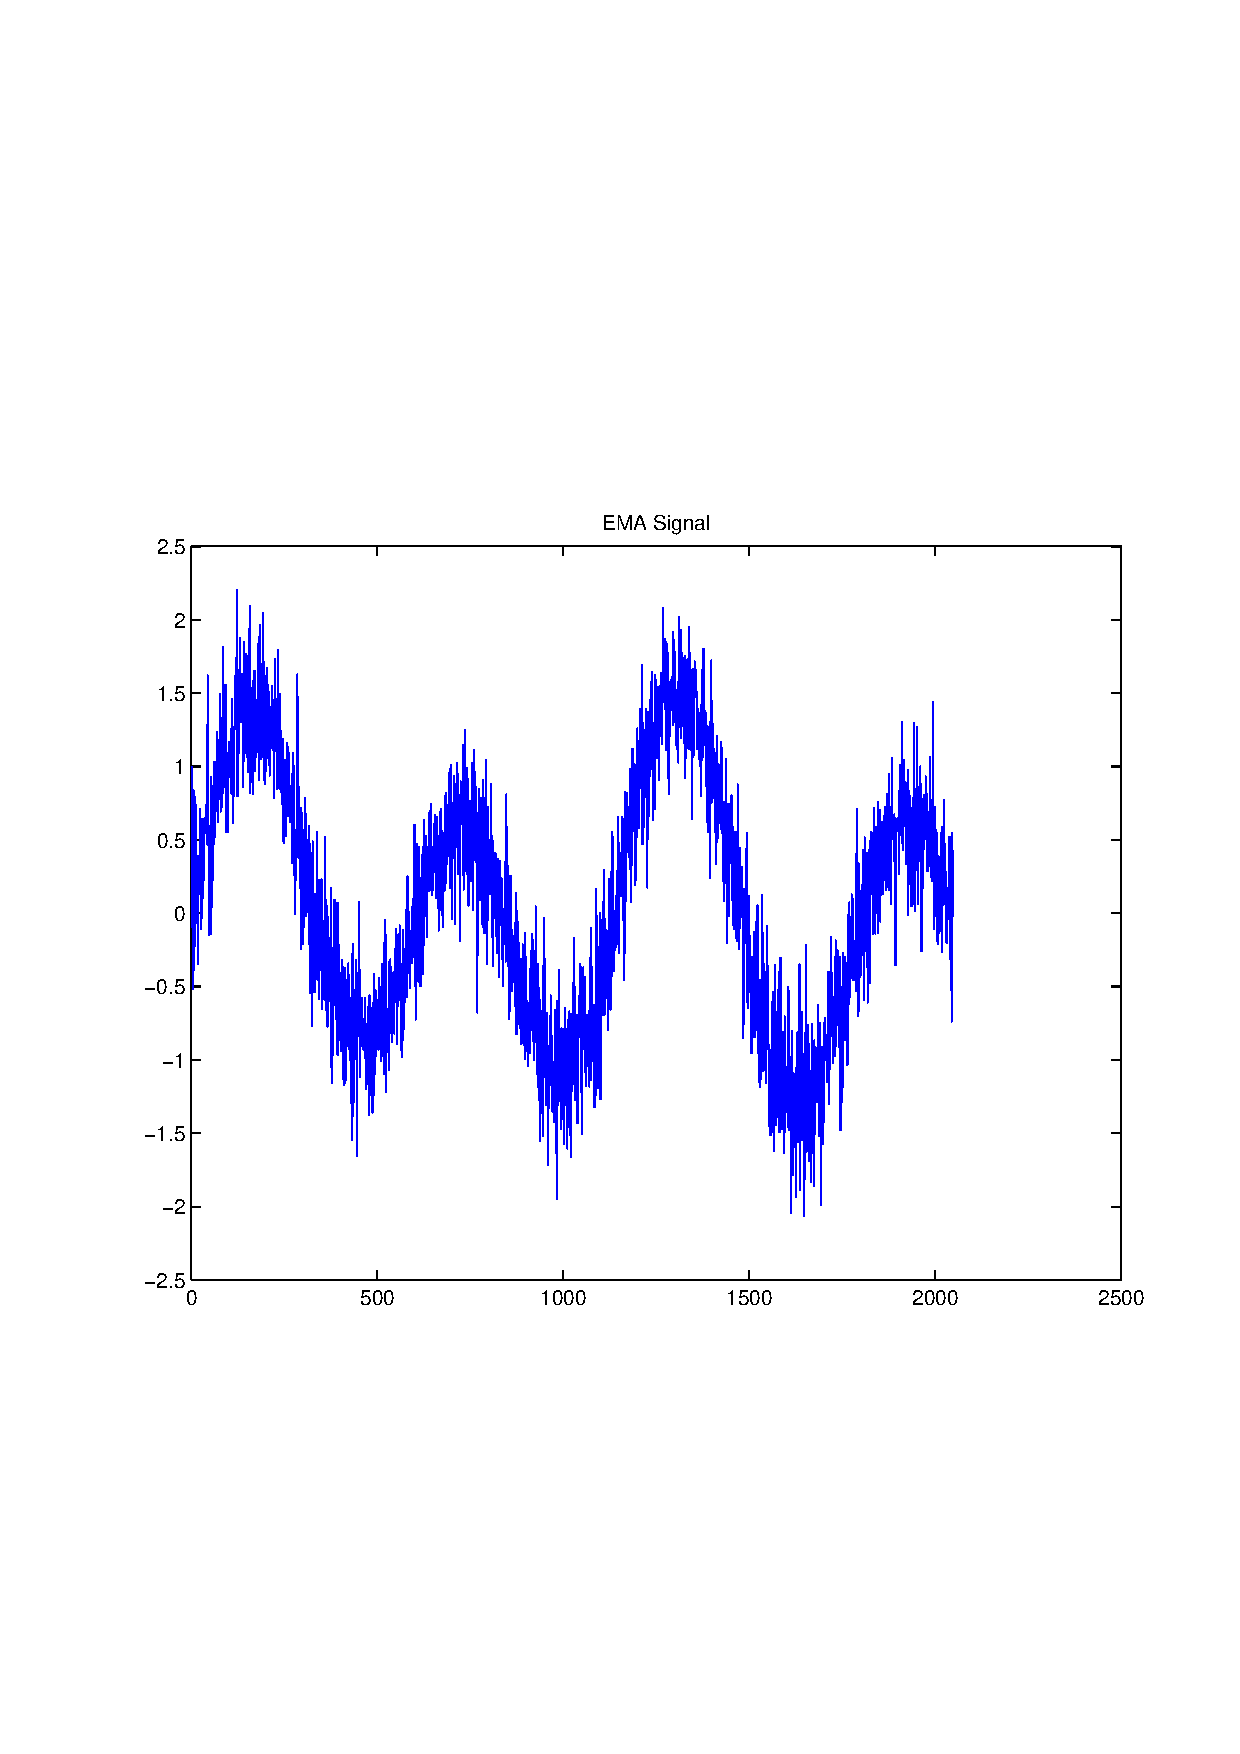
\includegraphics[width=10.0cm,height=10.0cm]{EMA_signal.pdf}

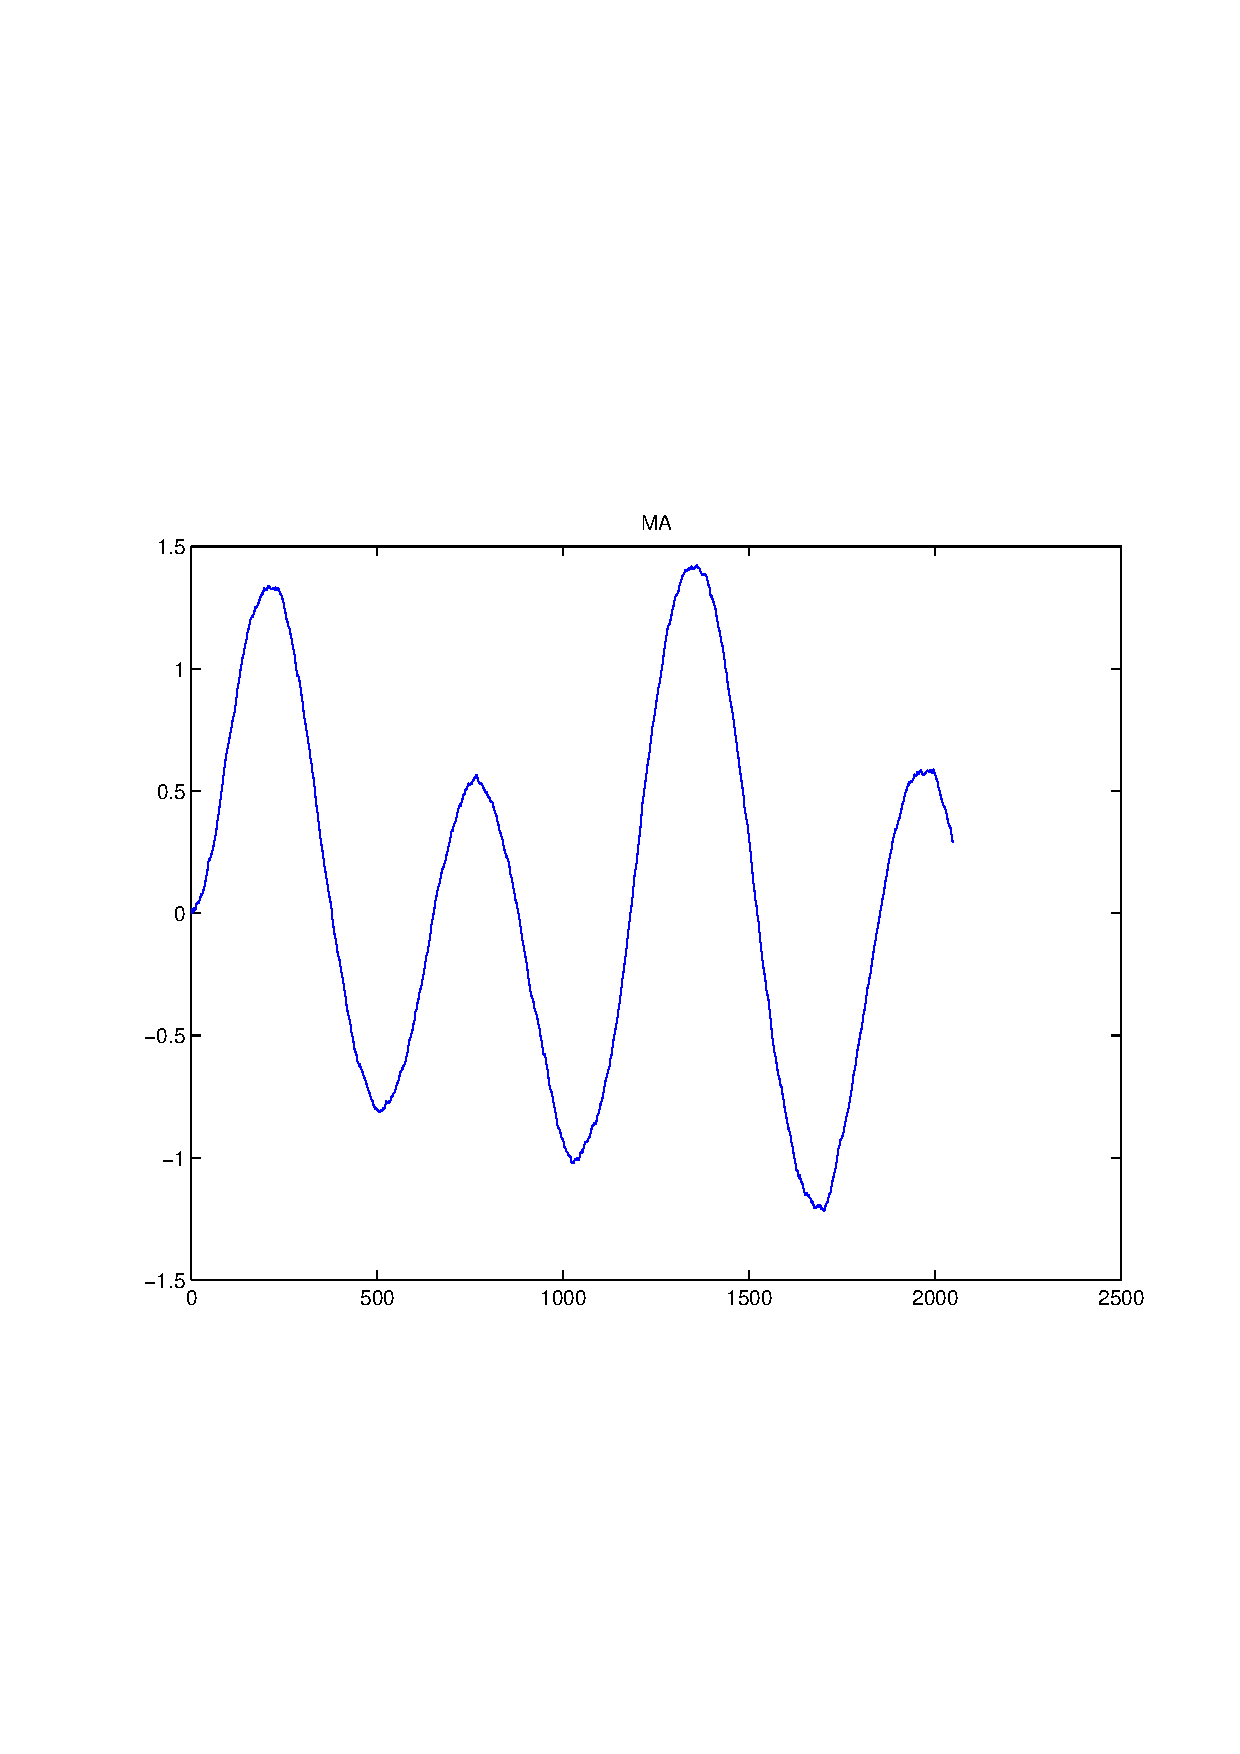
\includegraphics[width=10.0cm,height=10.0cm]{MA.pdf}

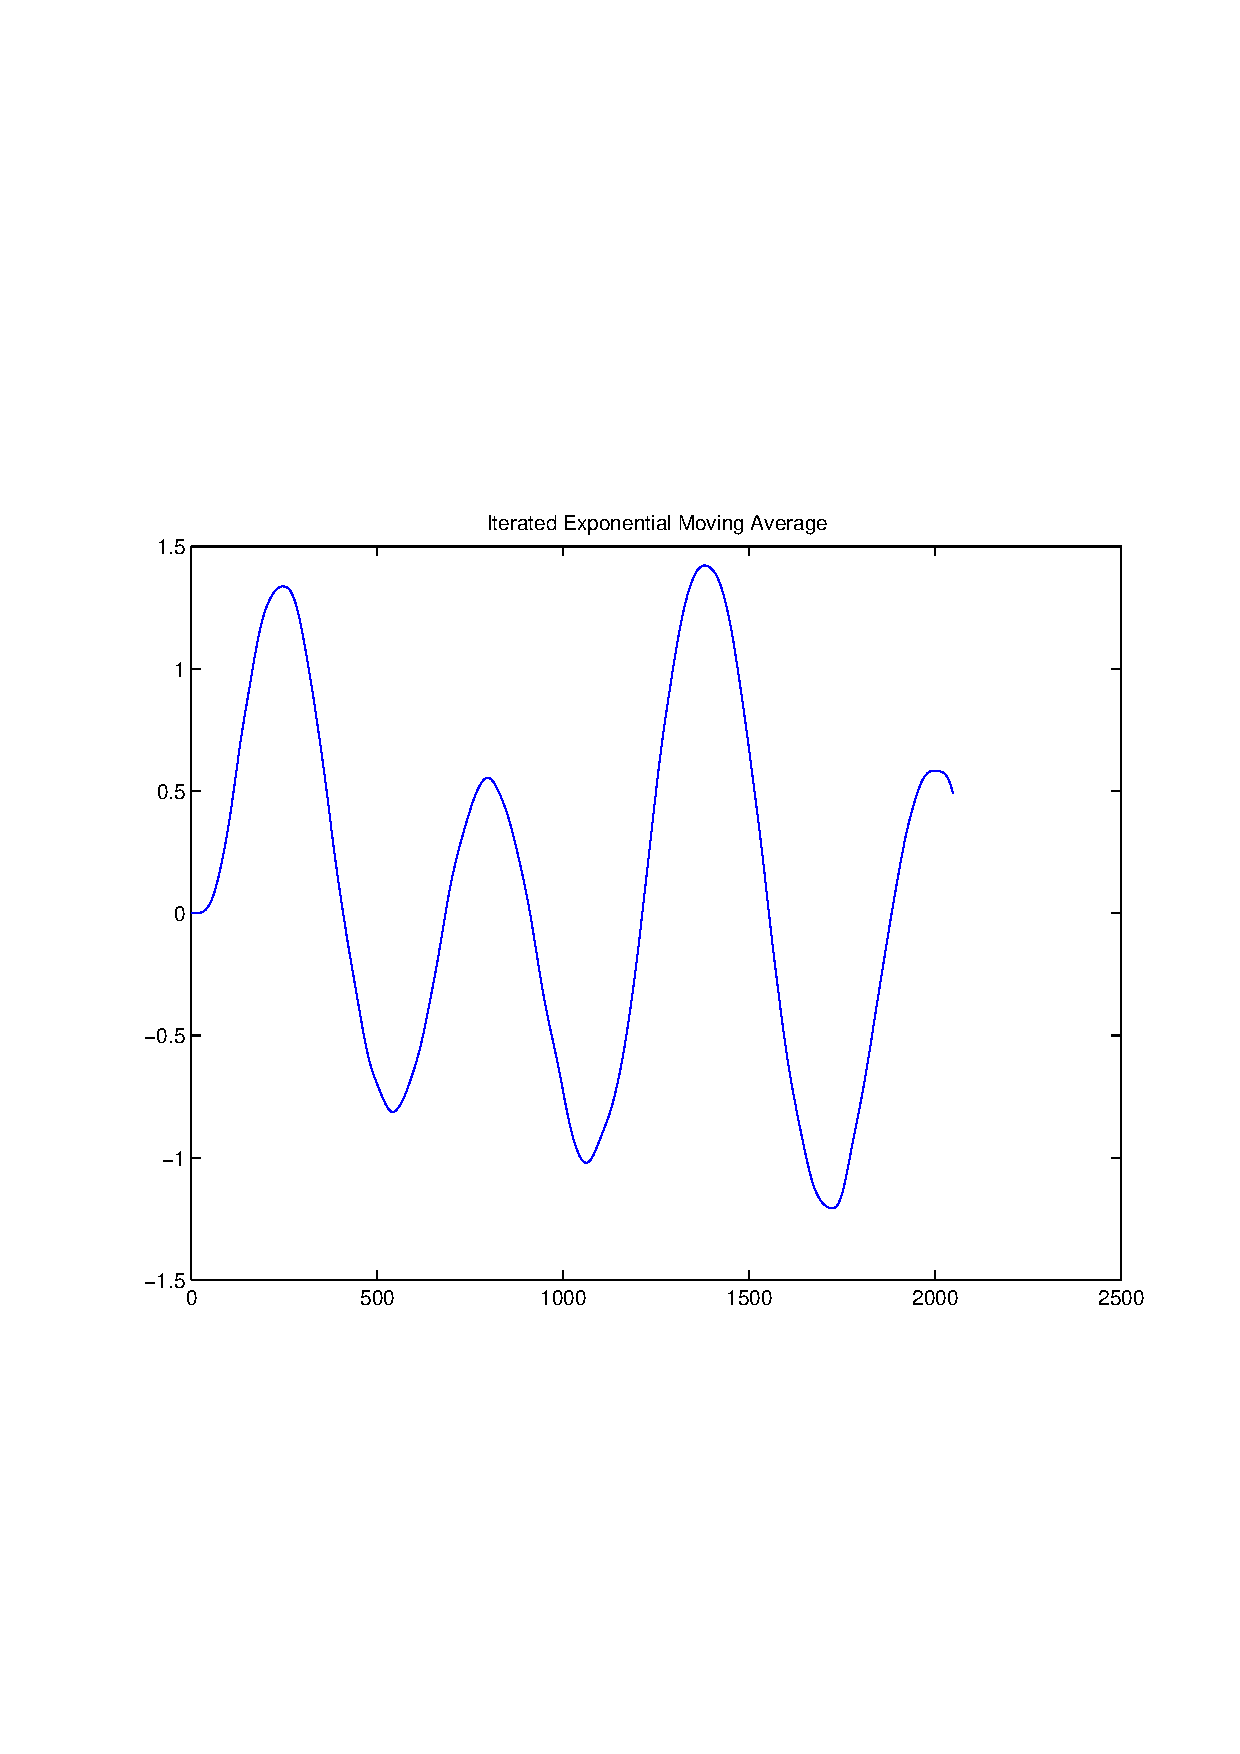
\includegraphics[width=10.0cm,height=10.0cm]{IEMA.pdf}

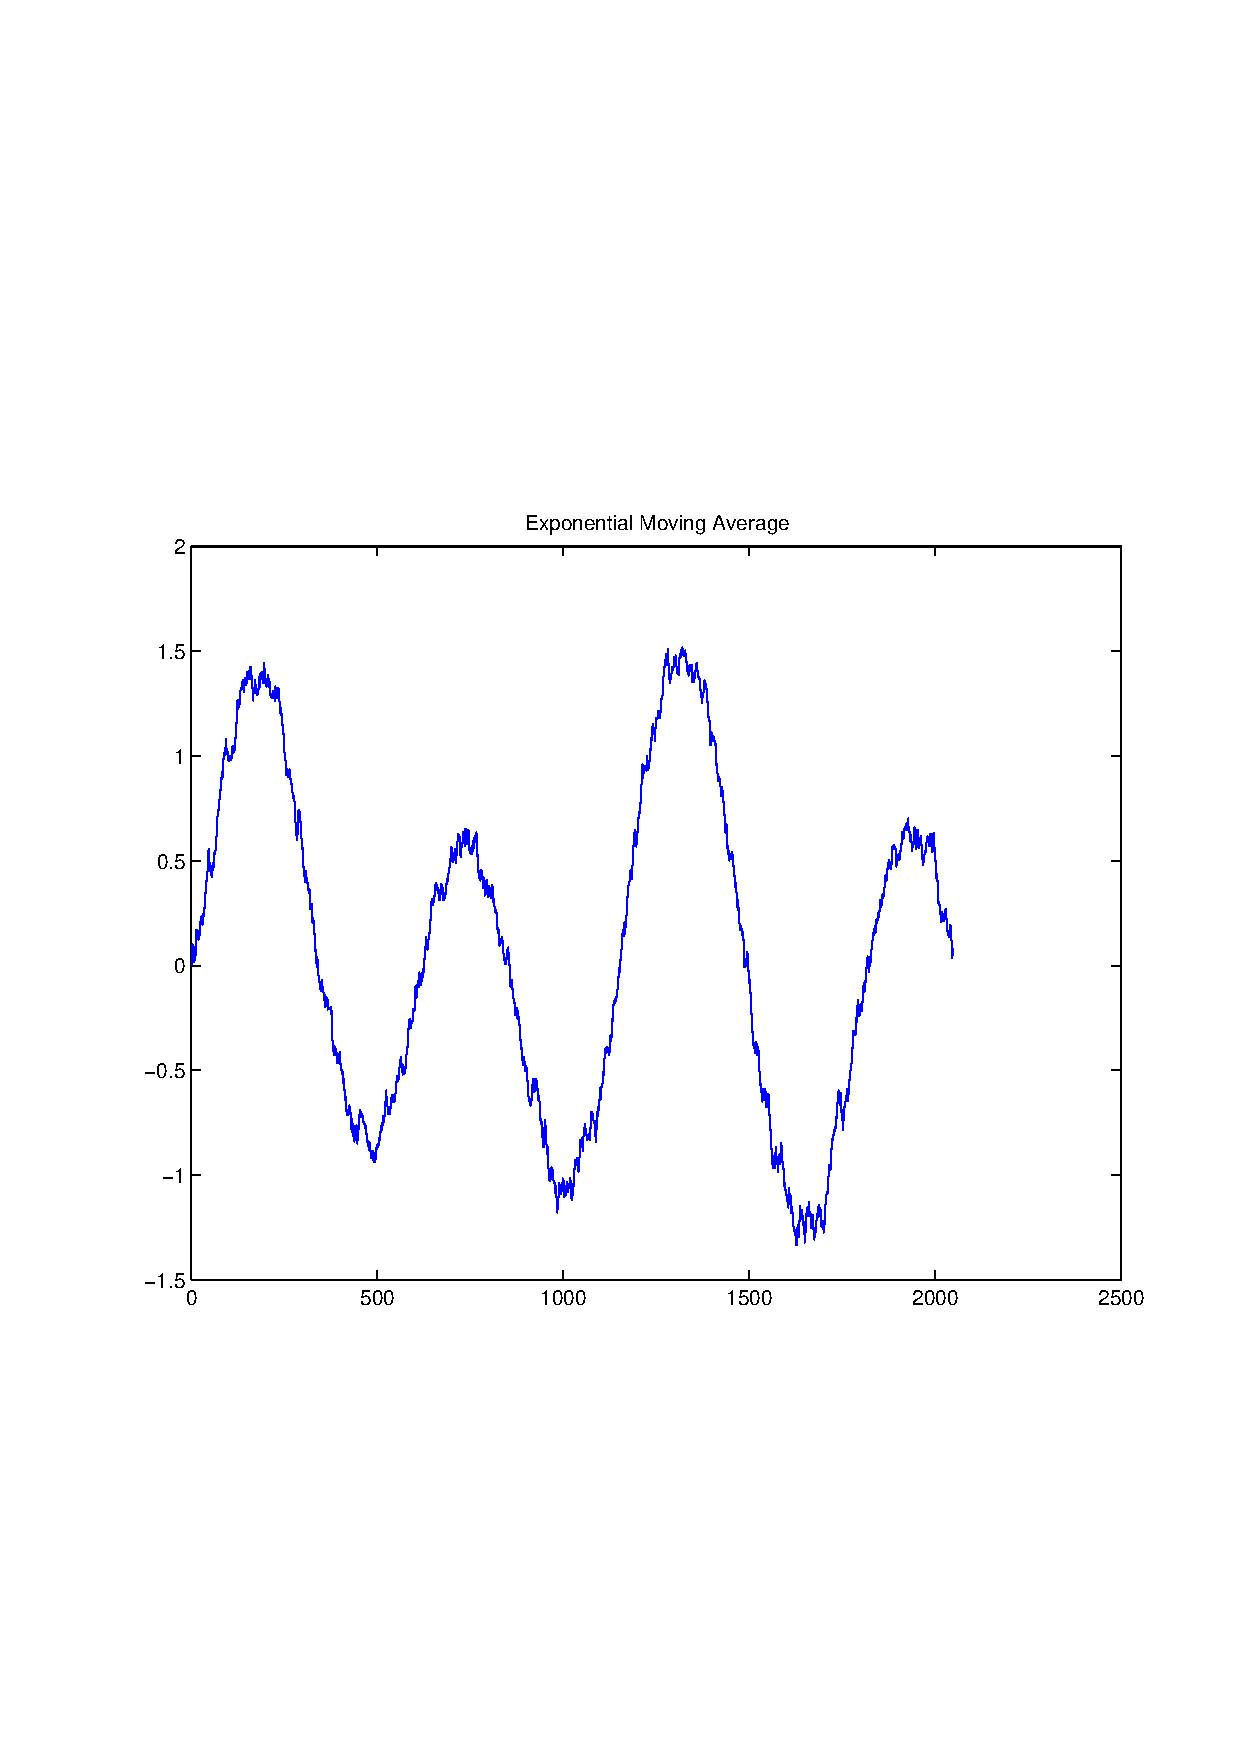
\includegraphics[width=10.0cm,height=10.0cm]{EMA.pdf}

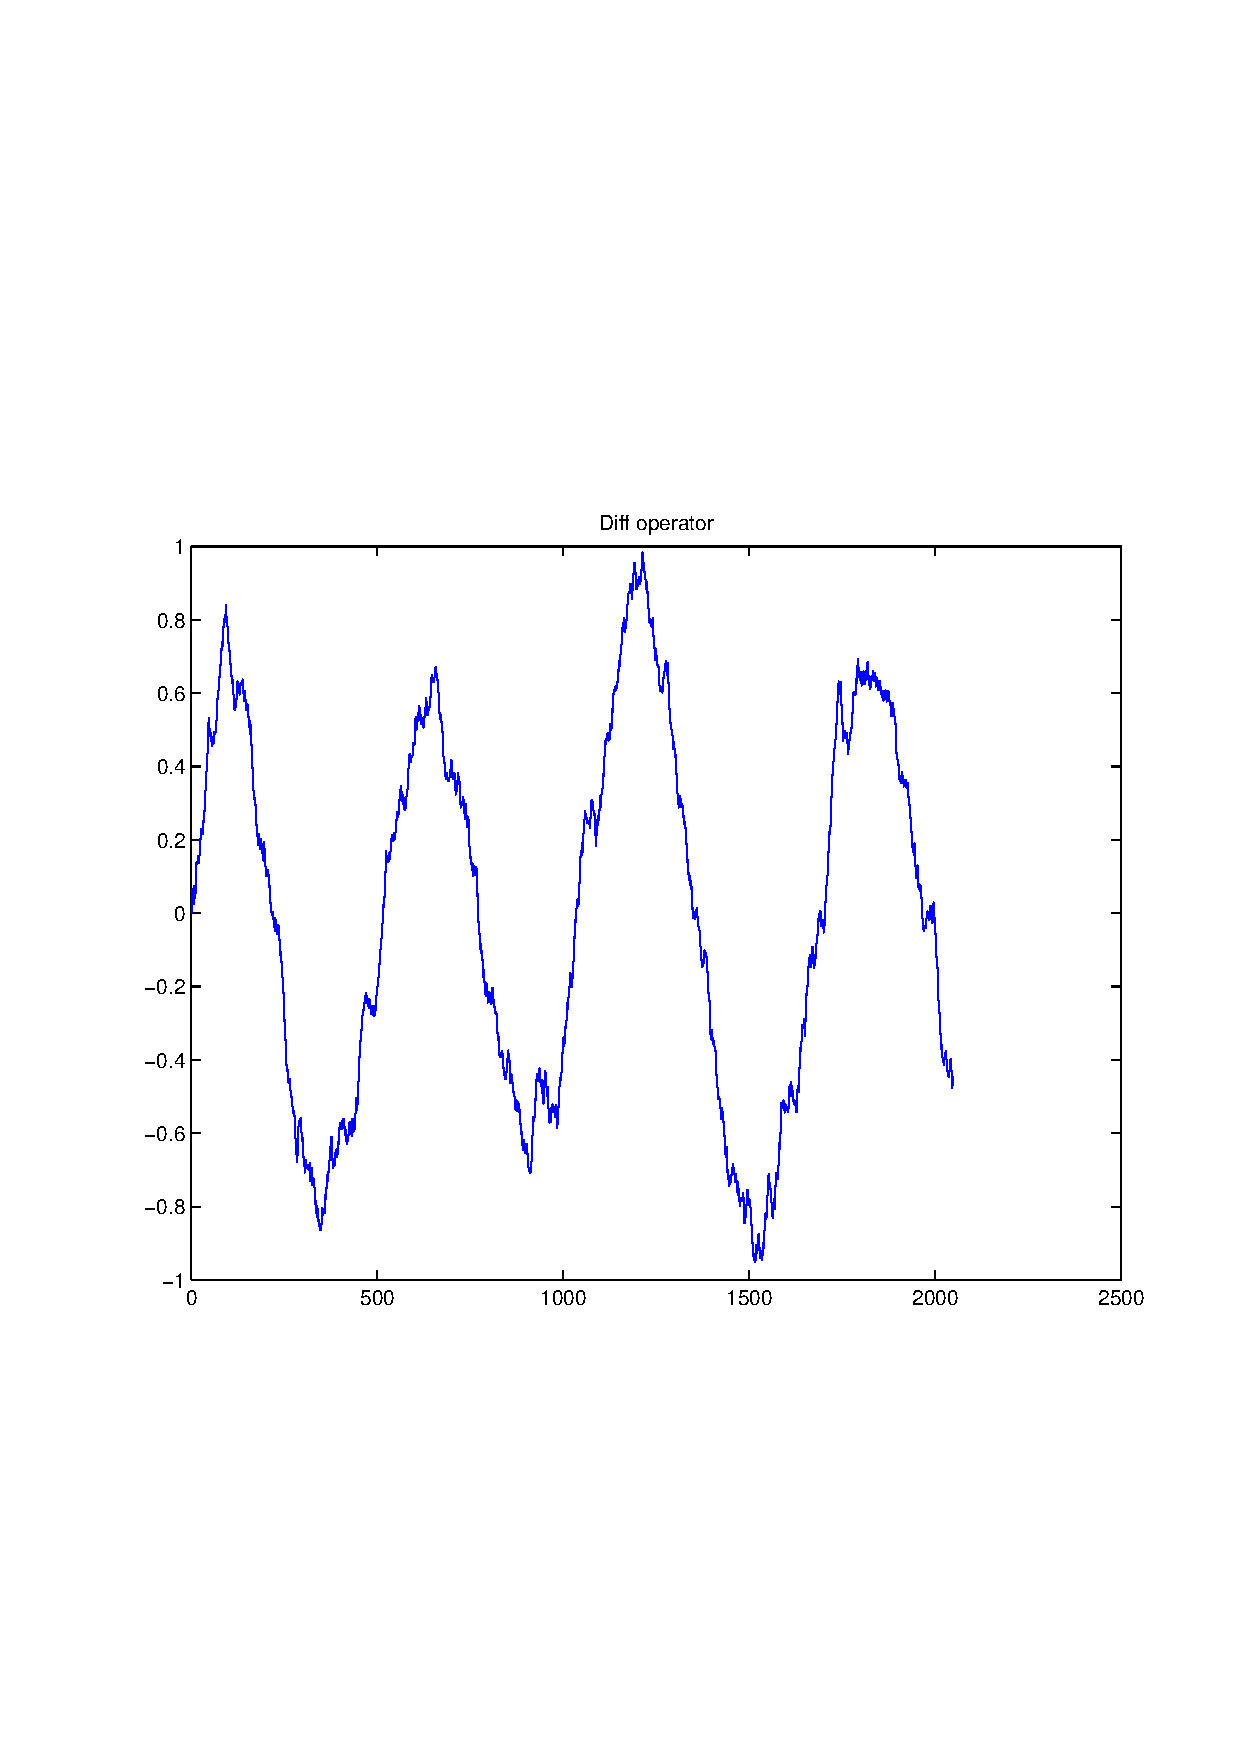
\includegraphics[width=10.0cm,height=10.0cm]{DIFF.pdf}

\includegraphics[width=10.0cm,height=10.0cm]{IteratedExponentailOperators.pdf}

\includegraphics[width=10.0cm,height=10.0cm]{IteratedExponentailOperators.pdf}

QueryPerformanceCounter  =  15.5227
\subsubsection{Testing binary writer}
Binary writer Speedup 1GB Double Matrix 23.1358
Binary reader Speedup 1GB Double Matrix 403.171
Binary writer Speedup 1GB Double vector 35.3458
Binary reader Speedup 1GB Double Matrix 293.216
QueryPerformanceCounter  =  4.48796
\subsubsection{Fast Gauss Transform}
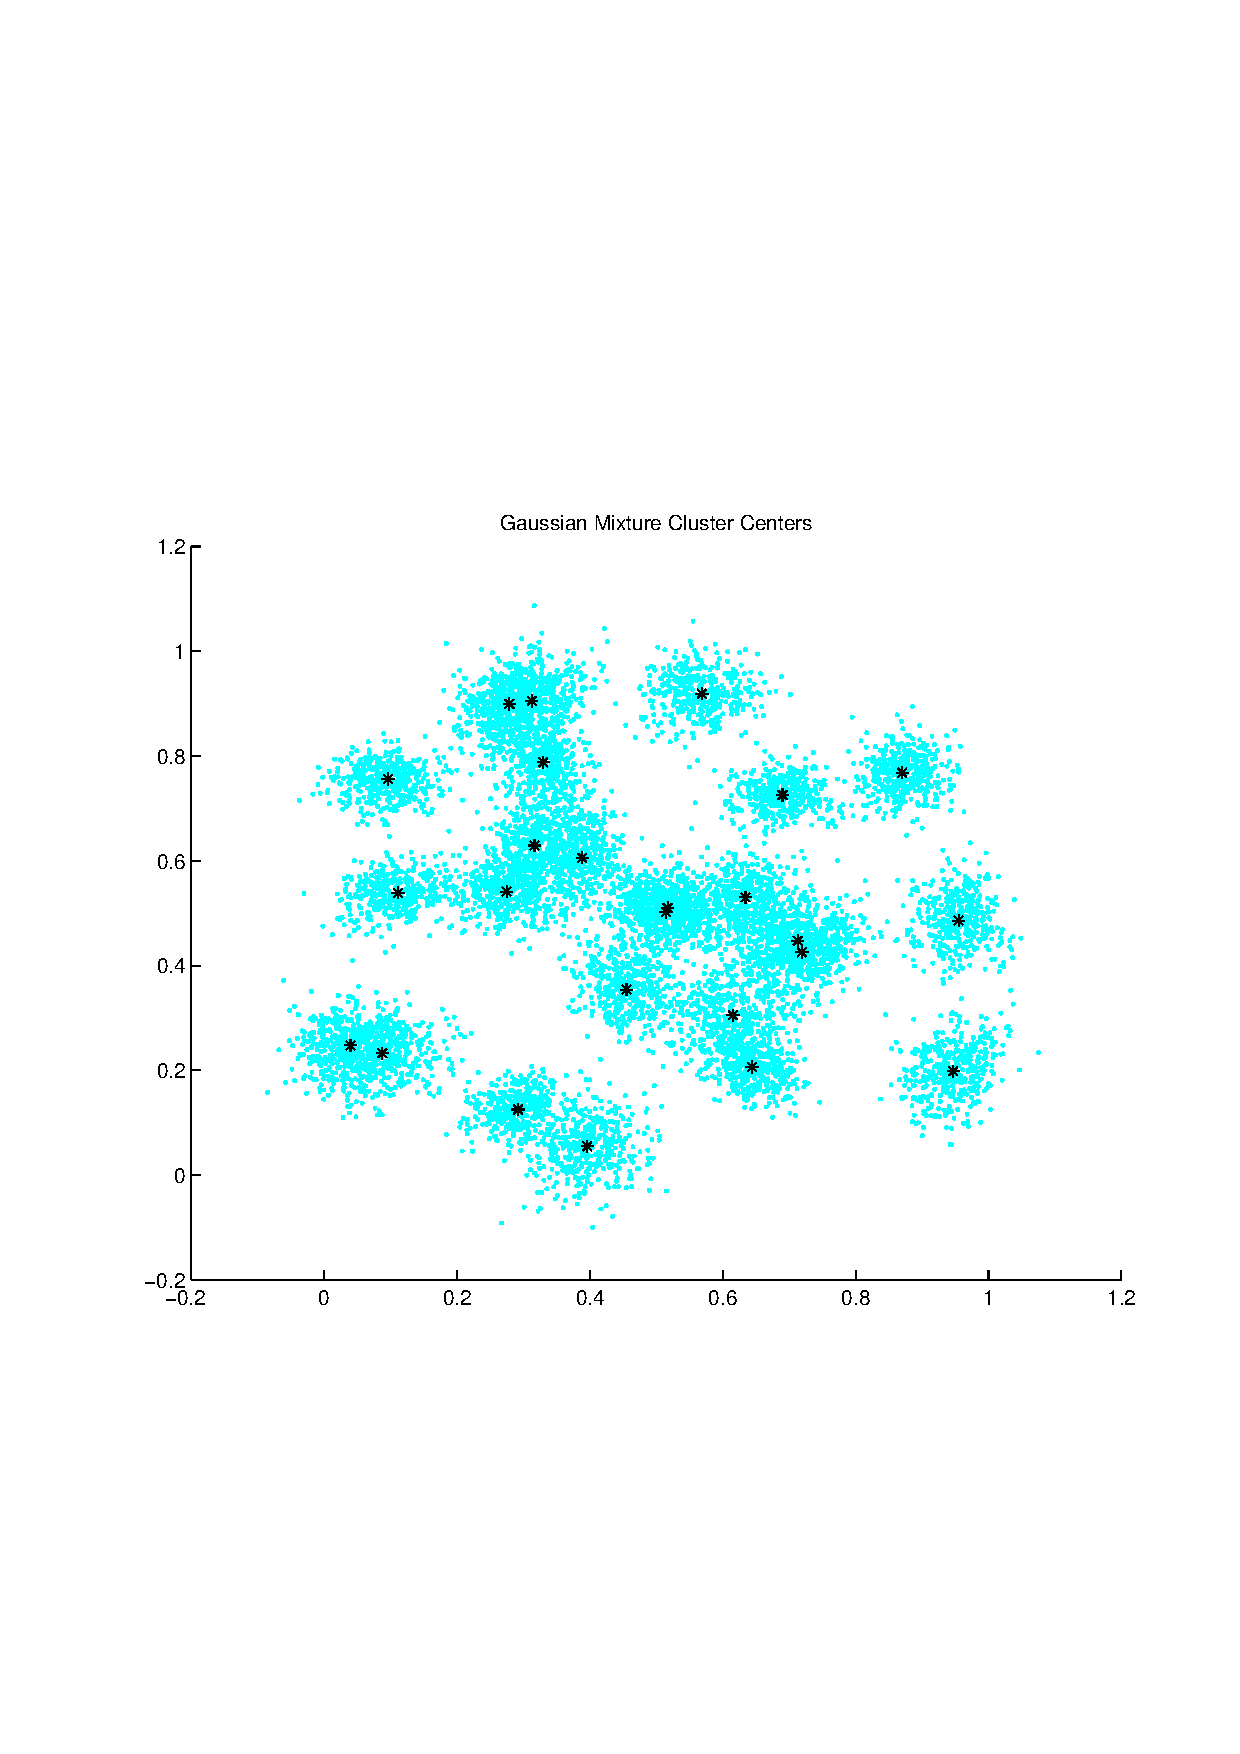
\includegraphics[width=10.0cm,height=10.0cm]{GaussianMixture_ClusterCenters25_Centers.pdf}

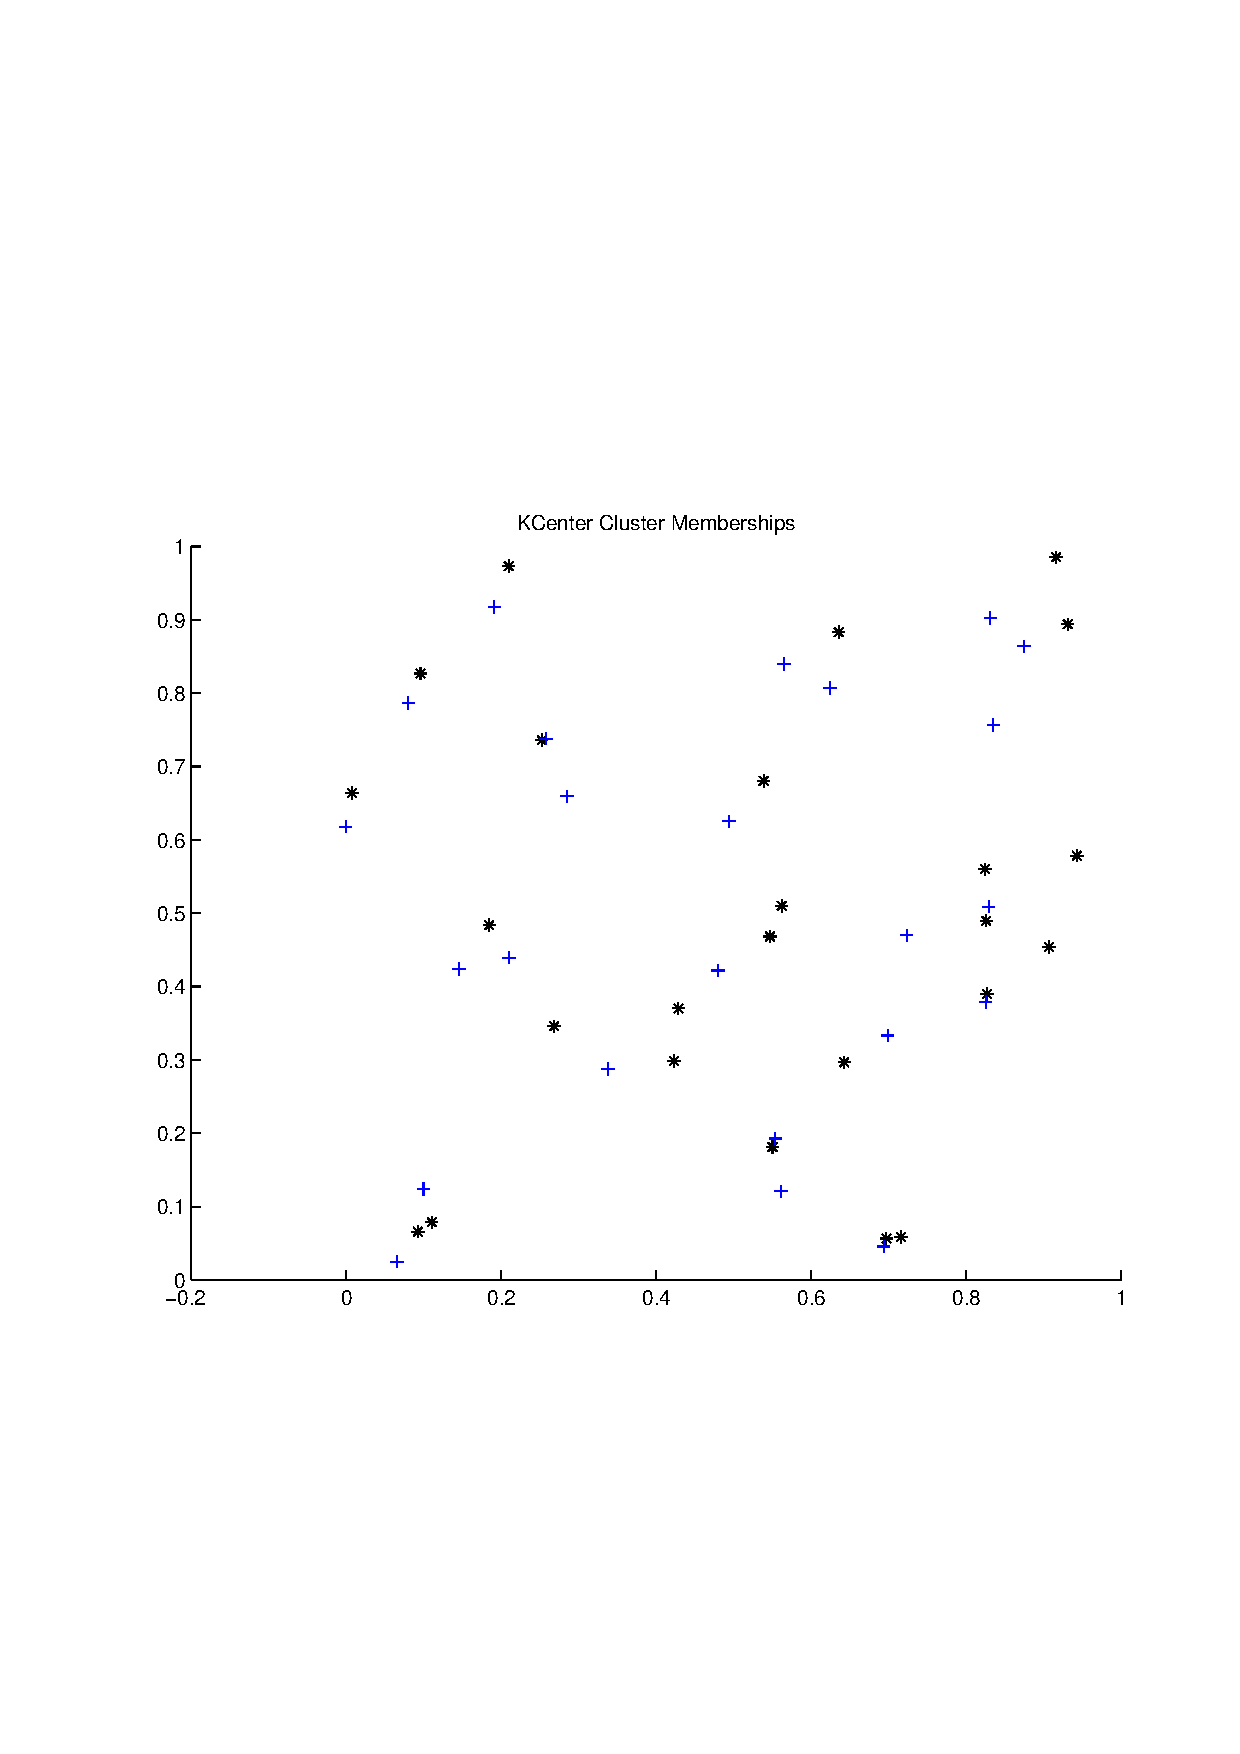
\includegraphics[width=10.0cm,height=10.0cm]{KCenterClusterMemberships_25_Centers.pdf}

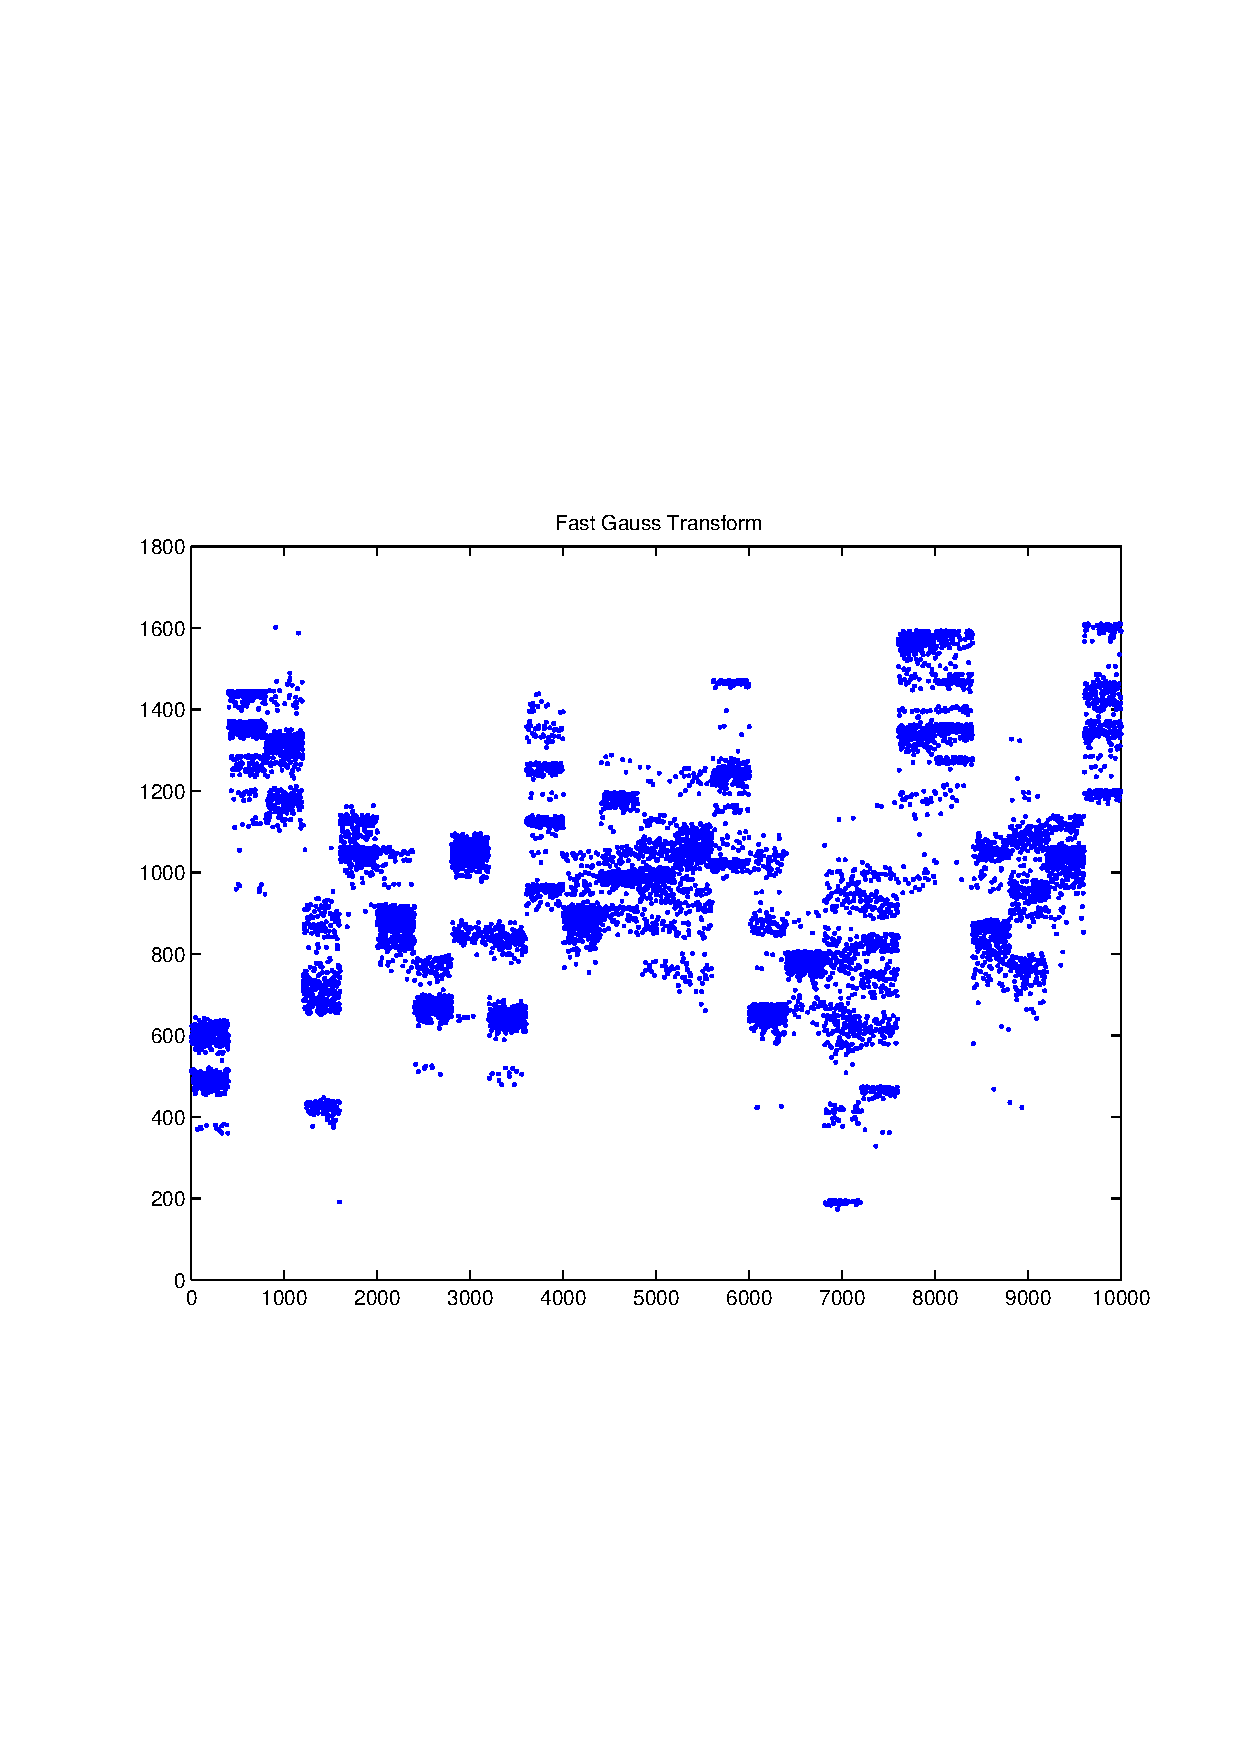
\includegraphics[width=10.0cm,height=10.0cm]{FGT25_Centers.pdf}

QueryPerformanceCounter  =  29.0737
\subsubsection{Testing Gaussian Mixture Point Cloud and Latex Plotting Capabilities.}
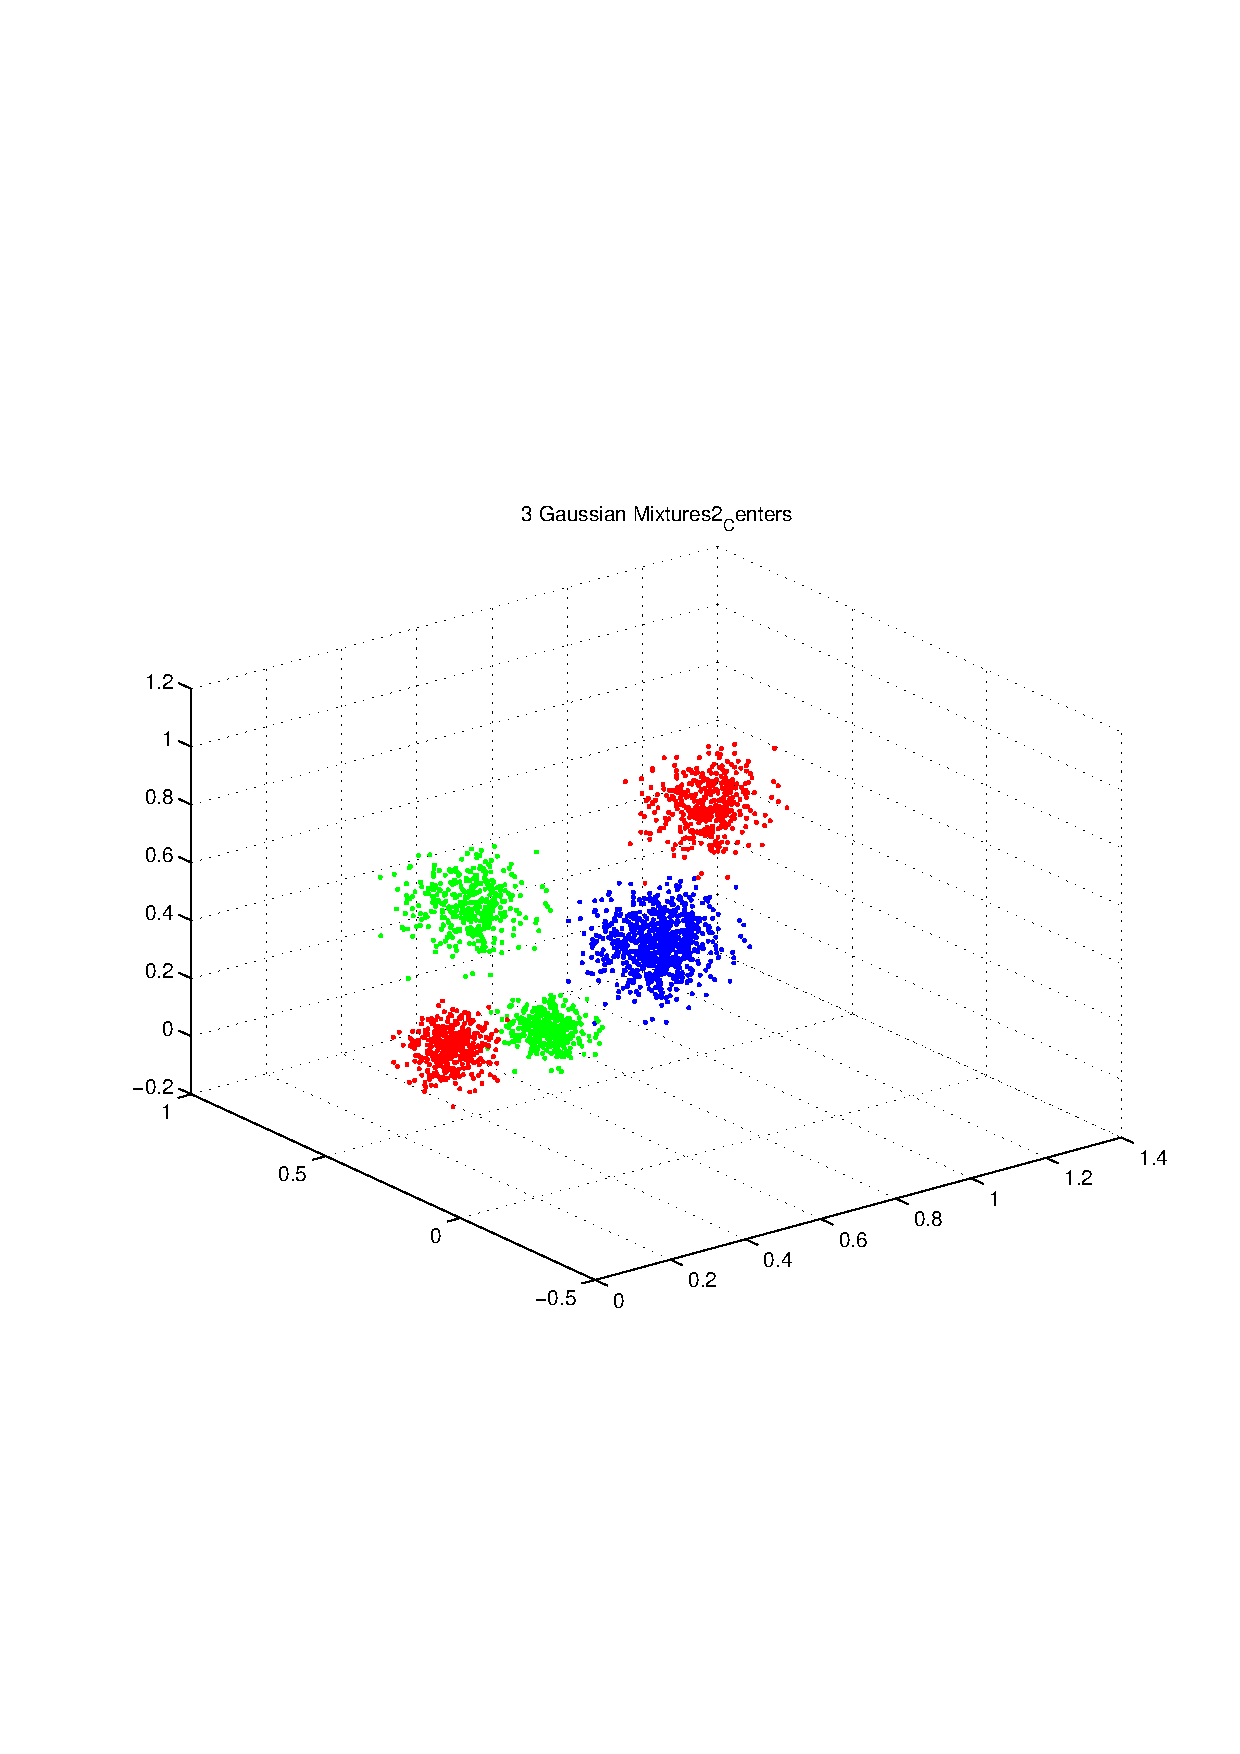
\includegraphics[width=10.0cm,height=10.0cm]{GaussianMixture_Dim_3_Centers2.pdf}

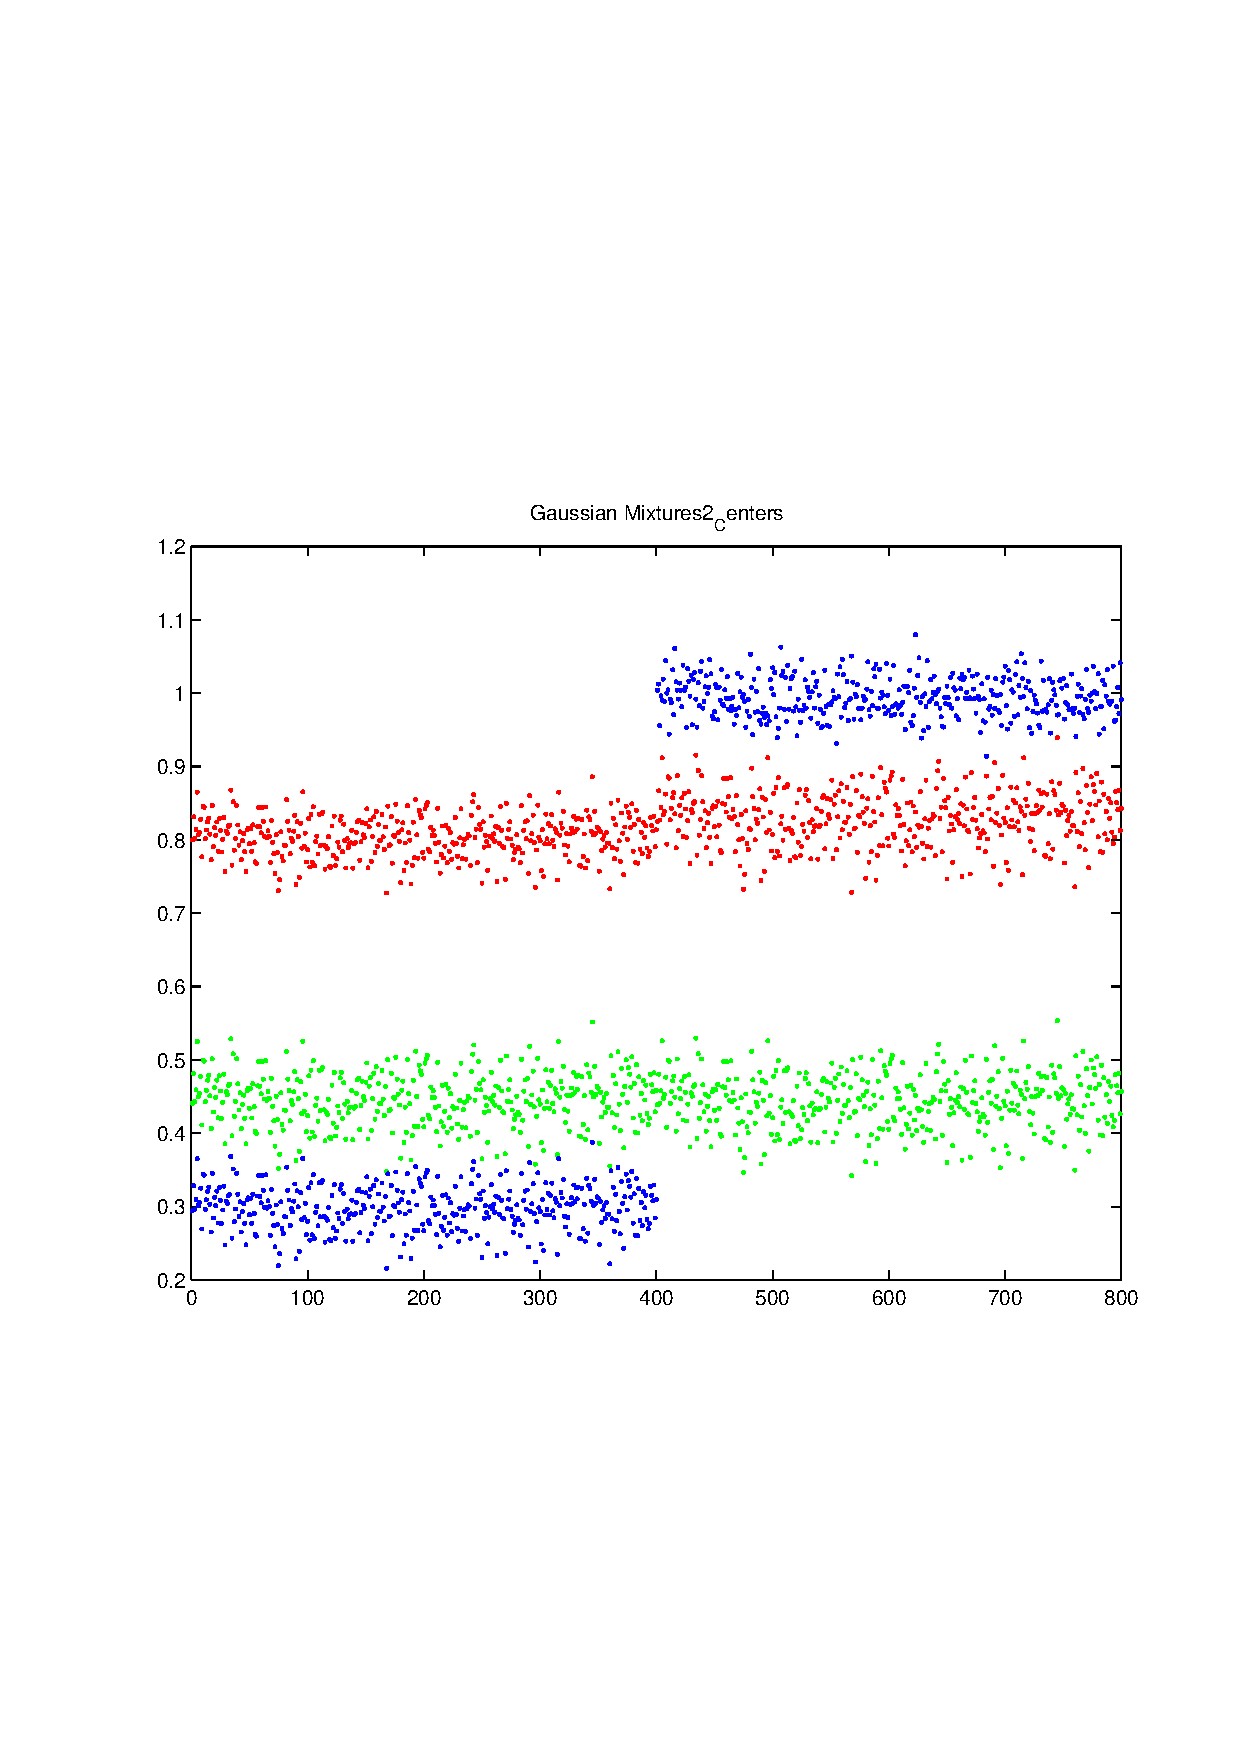
\includegraphics[width=10.0cm,height=10.0cm]{GaussianMixture_Dim_1_Centers2.pdf}

QueryPerformanceCounter  =  3.56236
\subsubsection{Matrix Quick Check <double>}
QueryPerformanceCounter  =  1.43159
\subsubsection{Matrix Quick Check <float>}
QueryPerformanceCounter  =  1.46924
\subsubsection{Intel VSL Function Check}
\includegraphics[width=10.0cm,height=10.0cm]{klVSLInv.pdf}

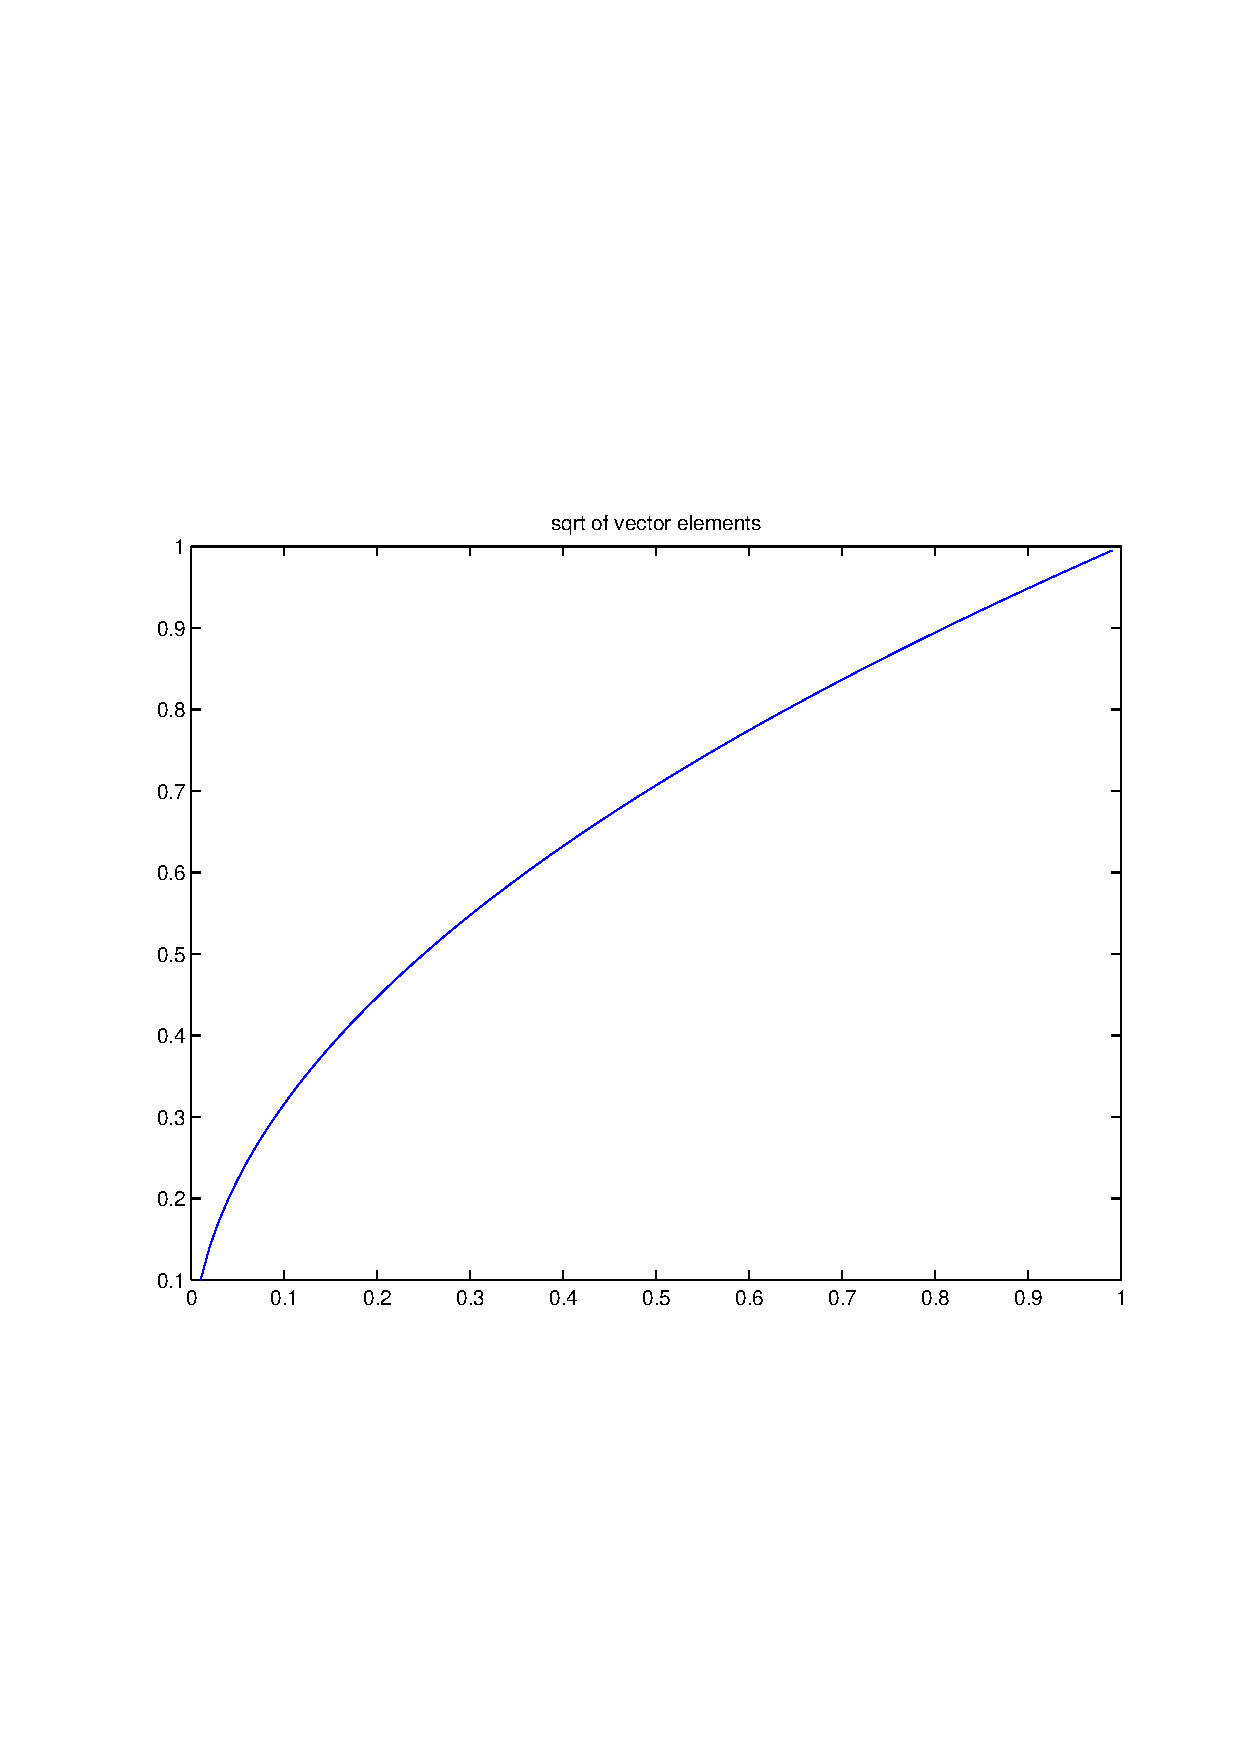
\includegraphics[width=10.0cm,height=10.0cm]{klVSLSqrt.pdf}

\includegraphics[width=10.0cm,height=10.0cm]{klVSLExp.pdf}

\includegraphics[width=10.0cm,height=10.0cm]{klVSLExpm1.pdf}

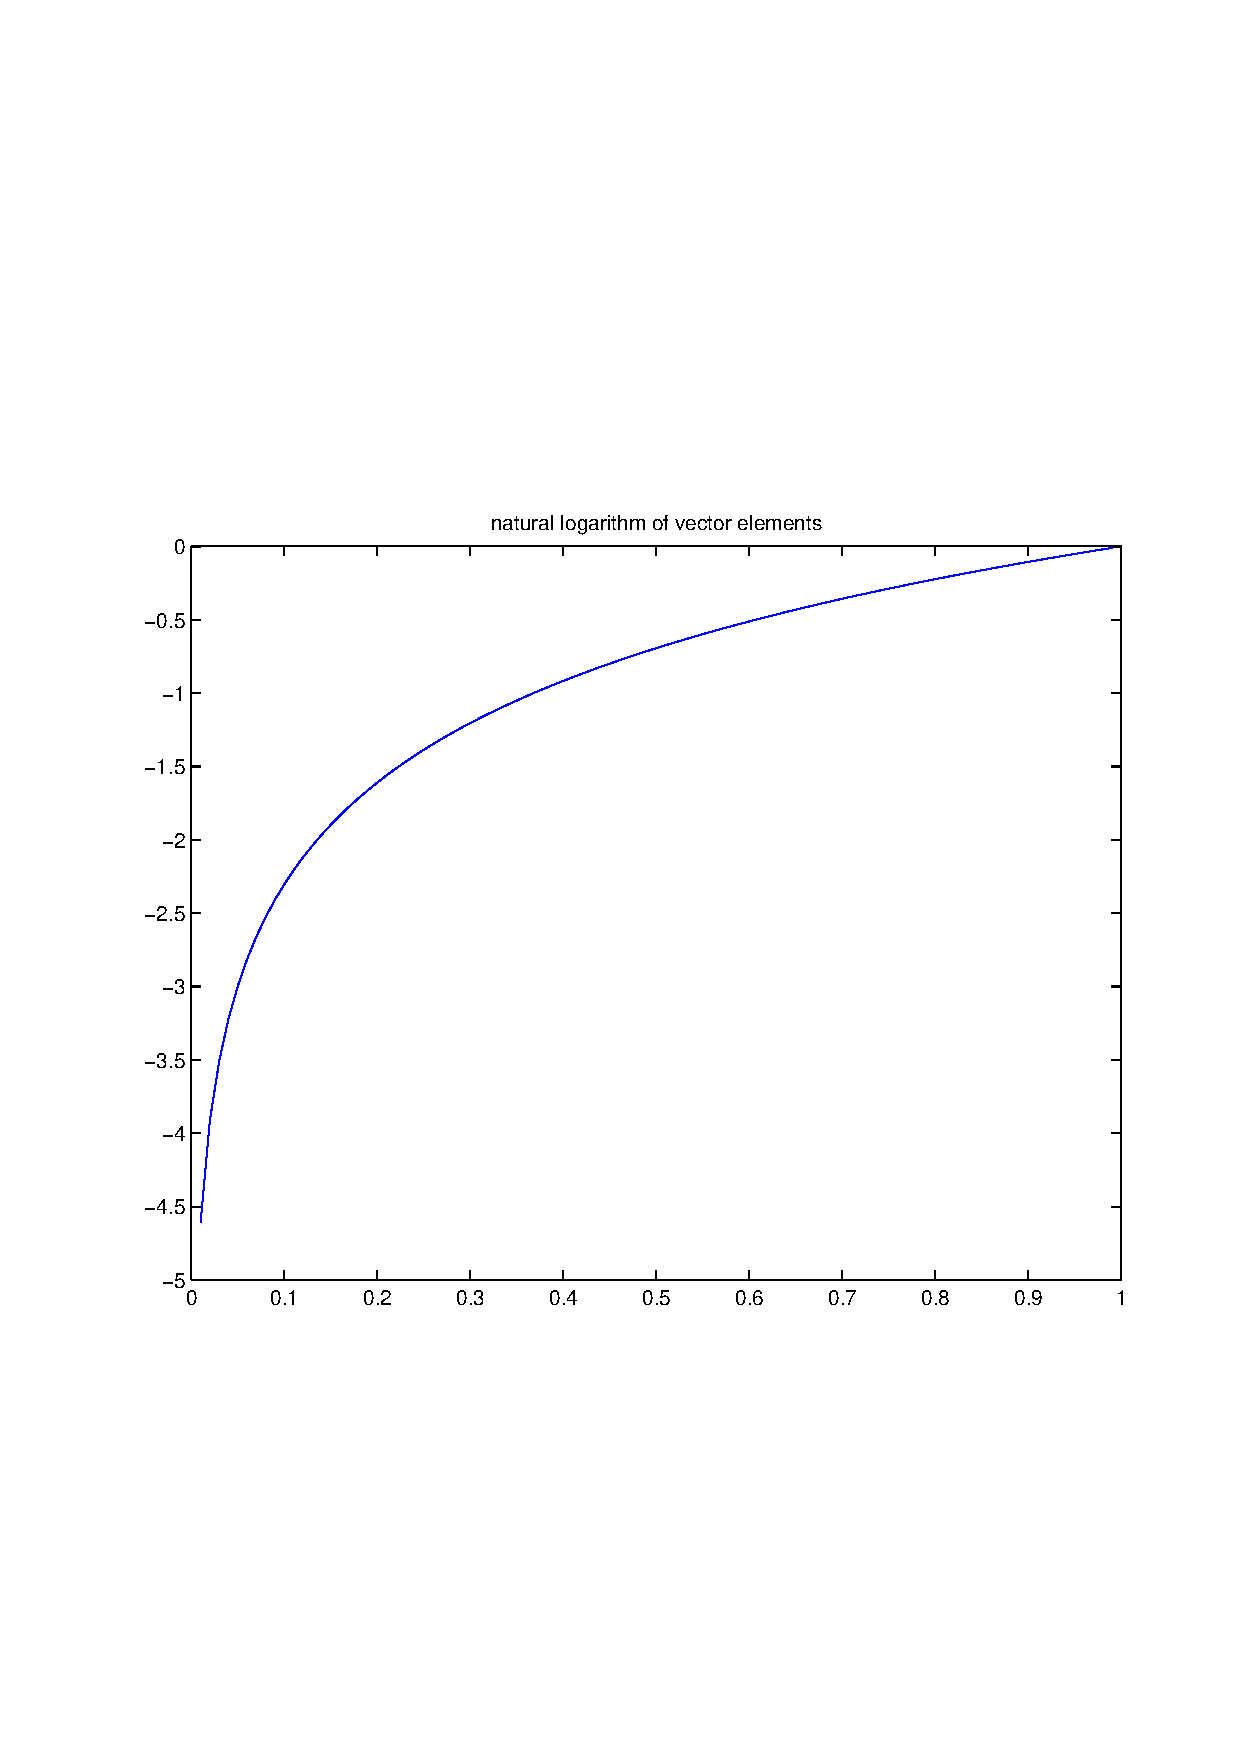
\includegraphics[width=10.0cm,height=10.0cm]{klVSLLn.pdf}

\includegraphics[width=10.0cm,height=10.0cm]{klVSLLog10.pdf}

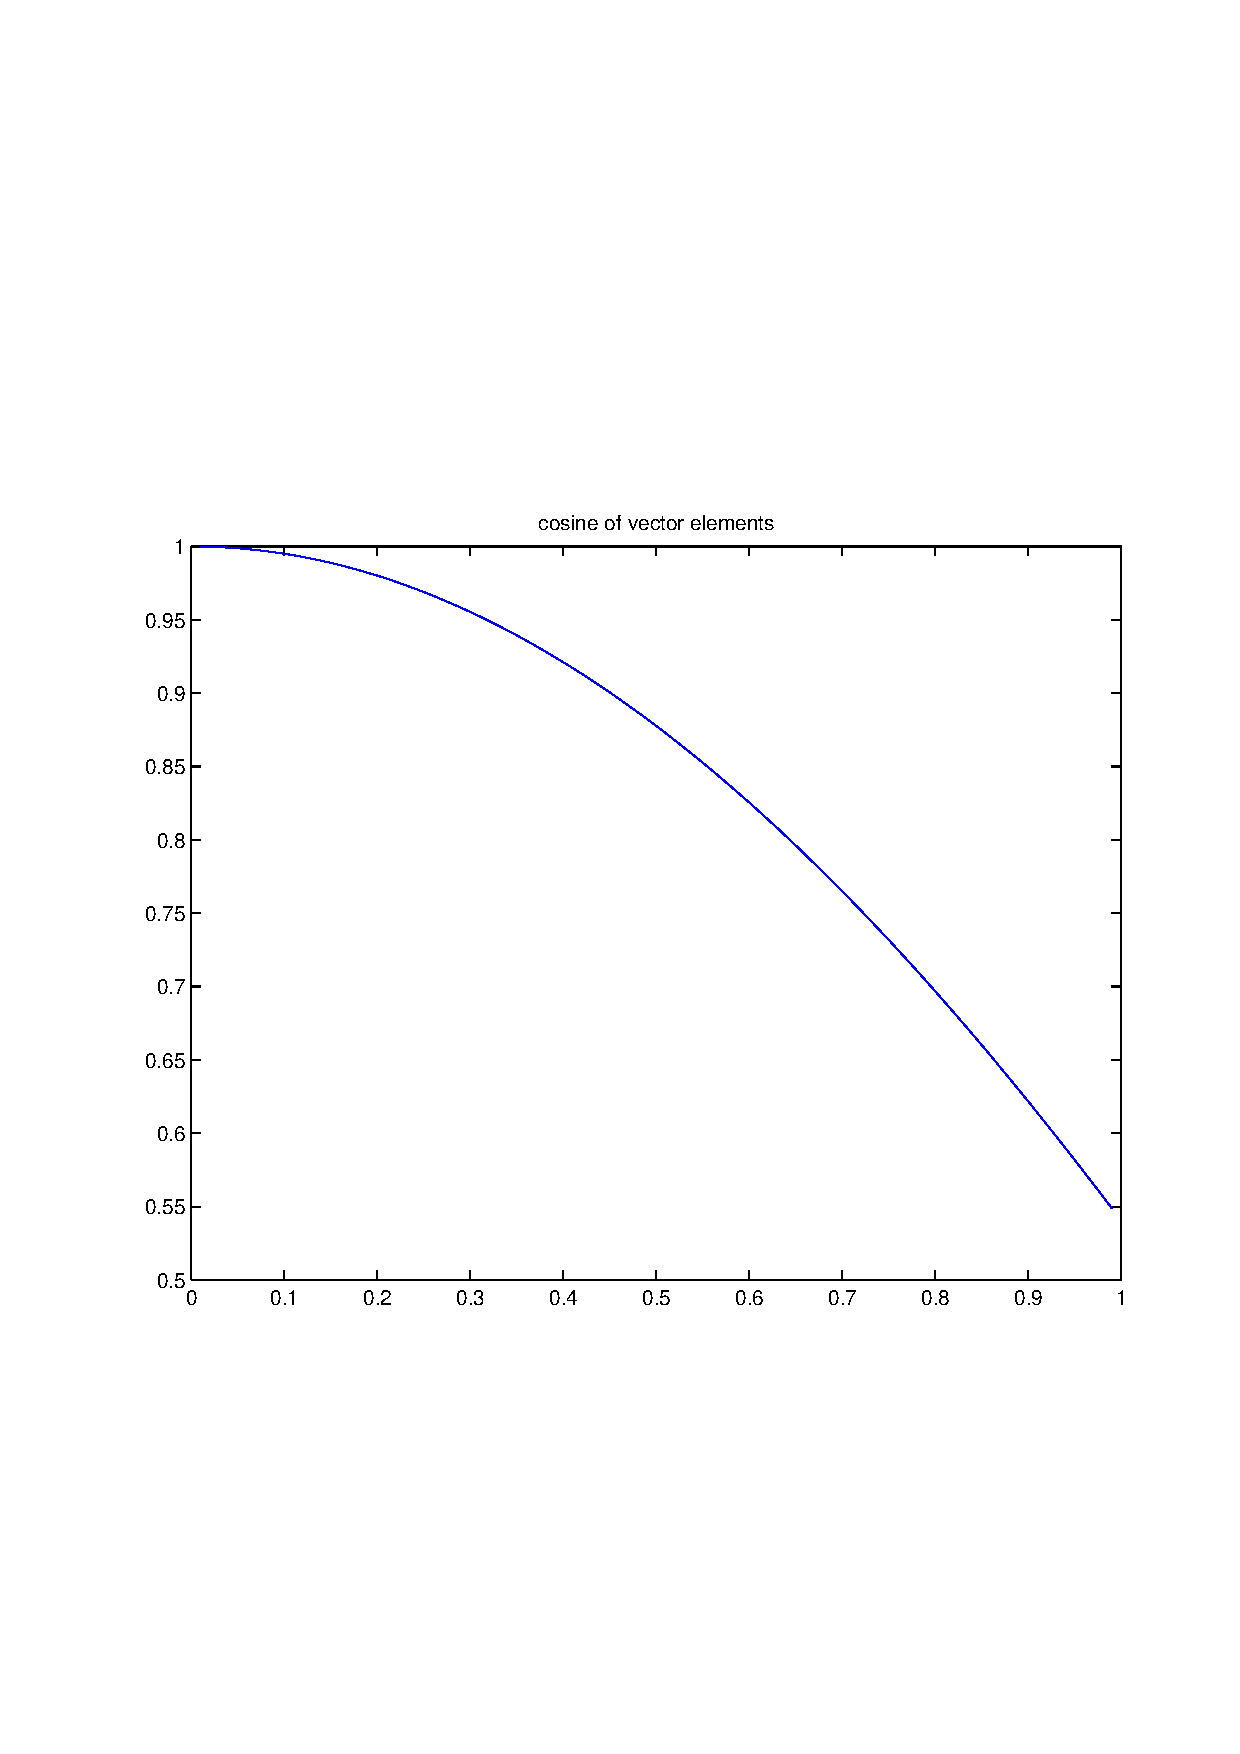
\includegraphics[width=10.0cm,height=10.0cm]{klVSLCos.pdf}

\includegraphics[width=10.0cm,height=10.0cm]{klVSLSin.pdf}

\includegraphics[width=10.0cm,height=10.0cm]{klVSLTan.pdf}

\includegraphics[width=10.0cm,height=10.0cm]{klVSLErf.pdf}

\includegraphics[width=10.0cm,height=10.0cm]{klVSLErfc.pdf}

\includegraphics[width=10.0cm,height=10.0cm]{klVSLCdfNorm.pdf}

\includegraphics[width=10.0cm,height=10.0cm]{klVSLErfInv.pdf}

\includegraphics[width=10.0cm,height=10.0cm]{klVSLLGamma.pdf}

\includegraphics[width=10.0cm,height=10.0cm]{klVSLTGamma.pdf}

QueryPerformanceCounter  =  14.5187
\subsubsection{Gram Matrix Consistency Check}
Sample Size = 4096
Feature dim = 3

$$Sigma$ = \left(
\begin{array}{
ccc}
+1.140 & +1.535 & +0.581 \\
+1.535 & +9.988 & +1.605 \\
+0.581 & +1.605 & +0.428 \\
\end{array}
\right)$ \newline 

$Sample Covariance = \left(
\begin{array}{
ccc}
+1.134 & +1.556 & +0.578 \\
+1.556 & +10.398 & +1.652 \\
+0.578 & +1.652 & +0.431 \\
\end{array}
\right)$ \newline 

$Sample Mean = \left(
\begin{array}{
ccc}
+1.00202 & +1.01805 & +1.00238 \\
\end{array}
\right)$ \newline 

$Sample Covariance-$Omega$ = \left(
\begin{array}{
ccc}
-0.005 & +0.021 & -0.003 \\
+0.021 & +0.409 & +0.047 \\
-0.003 & +0.047 & +0.003 \\
\end{array}
\right)$ \newline 

$Sample Covariance Eigs = \left(
\begin{array}{
ccc}
(+10.93523,+0.00000) & (+0.98703,+0.00000) & (+0.04042,+0.00000) \\
\end{array}
\right)$ \newline 

$Centered Mean = \left(
\begin{array}{
ccc}
+0.00000 & +0.00000 & +0.00000 \\
\end{array}
\right)$ \newline 

$Centered Covariance = \left(
\begin{array}{
ccc}
+1.134 & +1.556 & +0.578 \\
+1.556 & +10.398 & +1.652 \\
+0.578 & +1.652 & +0.431 \\
\end{array}
\right)$ \newline 

$Gram Matrix Gf Not scaled by sample size = \left(
\begin{array}{
ccc}
+4646.652 & +6372.887 & +2368.183 \\
+6372.887 & +42588.656 & +6765.707 \\
+2368.183 & +6765.707 & +1763.839 \\
\end{array}
\right)$ \newline 

$Gram Matrix Gf  scaled by sample size = \left(
\begin{array}{
ccc}
+1.134 & +1.556 & +0.578 \\
+1.556 & +10.398 & +1.652 \\
+0.578 & +1.652 & +0.431 \\
\end{array}
\right)$ \newline 

$SampleCovariance - Scaled Gf = \left(
\begin{array}{
ccc}
+0.000 & +0.000 & +0.000 \\
+0.000 & +0.003 & +0.000 \\
+0.000 & +0.000 & +0.000 \\
\end{array}
\right)$ \newline 

$EigenDecomp of SampleCovariance = \left(
\begin{array}{
ccc}
-0.164 & -0.973 & -0.162 \\
+0.920 & -0.210 & +0.331 \\
-0.357 & -0.095 & +0.929 \\
\end{array}
\right)$ \newline 

$EigenDecomp of Gram Matrix = \left(
\begin{array}{
ccc}
-0.114 & -0.976 & -0.186 \\
-0.309 & +0.213 & -0.927 \\
+0.944 & -0.048 & -0.326 \\
\end{array}
\right)$ \newline 

QueryPerformanceCounter  =  +59.529
\subsubsection{Eigen Solver Checks}
\subsubsection{Haar Distributed Random Orthogonal Matrix $A \in O(n)$}
 Testing Operator Norm
Number of Dimensions: +8

$A = \left(
\begin{array}{
cccccccc}
+0.388 & +0.202 & +0.318 & -0.054 & -0.330 & +0.303 & +0.220 & -0.675 \\
+0.483 & +0.015 & +0.411 & +0.269 & +0.316 & +0.408 & +0.067 & +0.505 \\
+0.424 & -0.052 & -0.419 & +0.301 & -0.149 & -0.389 & +0.606 & +0.103 \\
-0.191 & +0.301 & -0.225 & -0.386 & -0.433 & +0.457 & +0.311 & +0.424 \\
-0.372 & -0.113 & -0.202 & +0.141 & +0.556 & +0.402 & +0.485 & -0.287 \\
-0.474 & -0.254 & +0.504 & +0.443 & -0.415 & -0.081 & +0.265 & +0.106 \\
-0.190 & +0.887 & +0.099 & +0.290 & +0.165 & -0.234 & +0.024 & +0.003 \\
-0.011 & -0.016 & +0.447 & -0.621 & +0.269 & -0.398 & +0.421 & +0.076 \\
\end{array}
\right)$ \newline 

$Det(A) :   A \in O(n)$ = (+1.000,+0.000)

$L = \left(
\begin{array}{
cccccccc}
+1.000 & +0.000 & +0.000 & +0.000 & +0.000 & +0.000 & +0.000 & +0.000 \\
-0.393 & +1.000 & +0.000 & +0.000 & +0.000 & +0.000 & +0.000 & +0.000 \\
-0.982 & -0.269 & +1.000 & +0.000 & +0.000 & +0.000 & +0.000 & +0.000 \\
-0.022 & -0.018 & +0.472 & +1.000 & +0.000 & +0.000 & +0.000 & +0.000 \\
-0.770 & -0.114 & +0.147 & -0.276 & +1.000 & +0.000 & +0.000 & +0.000 \\
-0.396 & +0.344 & -0.156 & +0.291 & -0.542 & +1.000 & +0.000 & +0.000 \\
+0.878 & -0.073 & -0.778 & -0.733 & -0.230 & -0.702 & +1.000 & +0.000 \\
+0.803 & +0.213 & -0.069 & +0.301 & -0.802 & +0.521 & +0.153 & +1.000 \\
\end{array}
\right)$ \newline 

$U = \left(
\begin{array}{
cccccccc}
+0.483 & +0.015 & +0.411 & +0.269 & +0.316 & +0.408 & +0.067 & +0.505 \\
+0.000 & +0.893 & +0.261 & +0.396 & +0.289 & -0.074 & +0.051 & +0.202 \\
+0.000 & +0.000 & +0.977 & +0.813 & -0.027 & +0.299 & +0.344 & +0.656 \\
+0.000 & +0.000 & +0.000 & -0.991 & +0.294 & -0.532 & +0.261 & -0.219 \\
+0.000 & +0.000 & +0.000 & +0.000 & +0.917 & +0.517 & +0.563 & -0.032 \\
+0.000 & +0.000 & +0.000 & +0.000 & +0.000 & +1.126 & +0.603 & +0.703 \\
+0.000 & +0.000 & +0.000 & +0.000 & +0.000 & +0.000 & +1.563 & +0.511 \\
+0.000 & +0.000 & +0.000 & +0.000 & +0.000 & +0.000 & +0.000 & -1.483 \\
\end{array}
\right)$ \newline 

$L * U  = \left(
\begin{array}{
cccccccc}
+0.483 & +0.015 & +0.411 & +0.269 & +0.316 & +0.408 & +0.067 & +0.505 \\
-0.190 & +0.887 & +0.099 & +0.290 & +0.165 & -0.234 & +0.024 & +0.003 \\
-0.474 & -0.254 & +0.504 & +0.443 & -0.415 & -0.081 & +0.265 & +0.106 \\
-0.011 & -0.016 & +0.447 & -0.621 & +0.269 & -0.398 & +0.421 & +0.076 \\
-0.372 & -0.113 & -0.202 & +0.141 & +0.556 & +0.402 & +0.485 & -0.287 \\
-0.191 & +0.301 & -0.225 & -0.386 & -0.433 & +0.457 & +0.311 & +0.424 \\
+0.424 & -0.052 & -0.419 & +0.301 & -0.149 & -0.389 & +0.606 & +0.103 \\
+0.388 & +0.202 & +0.318 & -0.054 & -0.330 & +0.303 & +0.220 & -0.675 \\
\end{array}
\right)$ \newline 

$Det(L) :    = (+1.000,+0.000)     Det(U) :    = (+1.000,+0.000)     Det(LU) :    = (+1.000,+0.000)$

$||A||_{L_1}$  = +2.673

$||A||_{L_{\infty}}$ = +2.729

$||A^{-1}||_{L_1}$  = +2.729

$||A^{-1}||_{L_{\infty}}$ = +2.673

$||A||_{L_{\infty}} * ||A^{-1}||_{L_{\infty}} = +7.293$

$||A||_{L_1} * ||A^{-1}||_{L_1} = +7.293$

Frobenious Norm  $||A||_{\textit{F}}$ via $\sum\limits_{i,j =0}^{n} \|A_{i,j}|$   of  $A \in O(n)$  +2.828

$L_1$ condition number of Haar Distributed Random Orthogonal Matrix $A \in O(n)$ +6.608

$A = \left(
\begin{array}{
cccccccc}
+0.388 & +0.202 & +0.318 & -0.054 & -0.330 & +0.303 & +0.220 & -0.675 \\
+0.483 & +0.015 & +0.411 & +0.269 & +0.316 & +0.408 & +0.067 & +0.505 \\
+0.424 & -0.052 & -0.419 & +0.301 & -0.149 & -0.389 & +0.606 & +0.103 \\
-0.191 & +0.301 & -0.225 & -0.386 & -0.433 & +0.457 & +0.311 & +0.424 \\
-0.372 & -0.113 & -0.202 & +0.141 & +0.556 & +0.402 & +0.485 & -0.287 \\
-0.474 & -0.254 & +0.504 & +0.443 & -0.415 & -0.081 & +0.265 & +0.106 \\
-0.190 & +0.887 & +0.099 & +0.290 & +0.165 & -0.234 & +0.024 & +0.003 \\
-0.011 & -0.016 & +0.447 & -0.621 & +0.269 & -0.398 & +0.421 & +0.076 \\
\end{array}
\right)$ \newline 

$L_{\infty}$ condition number of Haar Distributed Random Orthogonal Matrix $A \in O(n)$ +6.547

Eigenvalues of $A \in O(n)$

(-0.885,+0.465), (-0.885,-0.465), (+0.361,+0.933), (+0.361,-0.933), (-0.389,+0.921), (-0.389,-0.921), (+1.000,+0.002), (+1.000,-0.002)

 $|\lambda | : \lambda \in \sigma(A) , A \in O(n)$

+1.000, +1.000, +1.000, +1.000, +1.000, +1.000, +1.000, +1.000


Calculating $A^{\dag} A,$  we expect $A^{\dag} A \approx I$

$A^{\dag} A = \left(
\begin{array}{
cccccccc}
+1.000 & -0.000 & +0.000 & +0.000 & -0.000 & +0.000 & +0.000 & -0.000 \\
-0.000 & +1.000 & -0.000 & -0.000 & -0.000 & -0.000 & -0.000 & -0.000 \\
+0.000 & -0.000 & +1.000 & +0.000 & +0.000 & +0.000 & +0.000 & +0.000 \\
+0.000 & -0.000 & +0.000 & +1.000 & +0.000 & -0.000 & -0.000 & -0.000 \\
-0.000 & -0.000 & +0.000 & +0.000 & +1.000 & +0.000 & -0.000 & +0.000 \\
+0.000 & -0.000 & +0.000 & -0.000 & +0.000 & +1.000 & -0.000 & +0.000 \\
+0.000 & -0.000 & +0.000 & -0.000 & -0.000 & -0.000 & +1.000 & +0.000 \\
-0.000 & -0.000 & +0.000 & -0.000 & +0.000 & +0.000 & +0.000 & +1.000 \\
\end{array}
\right)$ \newline 

Calculating $A^{-1} ,  A \in O(n)$.

$A^{-1} = \left(
\begin{array}{
cccccccc}
+0.388 & +0.483 & +0.424 & -0.191 & -0.372 & -0.474 & -0.190 & -0.011 \\
+0.202 & +0.015 & -0.052 & +0.301 & -0.113 & -0.254 & +0.887 & -0.016 \\
+0.318 & +0.411 & -0.419 & -0.225 & -0.202 & +0.504 & +0.099 & +0.447 \\
-0.054 & +0.269 & +0.301 & -0.386 & +0.141 & +0.443 & +0.290 & -0.621 \\
-0.330 & +0.316 & -0.149 & -0.433 & +0.556 & -0.415 & +0.165 & +0.269 \\
+0.303 & +0.408 & -0.389 & +0.457 & +0.402 & -0.081 & -0.234 & -0.398 \\
+0.220 & +0.067 & +0.606 & +0.311 & +0.485 & +0.265 & +0.024 & +0.421 \\
-0.675 & +0.505 & +0.103 & +0.424 & -0.287 & +0.106 & +0.003 & +0.076 \\
\end{array}
\right)$ \newline 

Calculating $A^{-1} *A  ,  A \in O(n)$.   We expect $A^{-1} *A  \approx I$. 

$A^{-1} *A = \left(
\begin{array}{
cccccccc}
+1.000 & +0.000 & +0.000 & -0.000 & +0.000 & +0.000 & +0.000 & +0.000 \\
+0.000 & +1.000 & +0.000 & -0.000 & +0.000 & +0.000 & +0.000 & -0.000 \\
-0.000 & +0.000 & +1.000 & -0.000 & +0.000 & -0.000 & +0.000 & -0.000 \\
+0.000 & -0.000 & +0.000 & +1.000 & +0.000 & +0.000 & +0.000 & +0.000 \\
-0.000 & -0.000 & +0.000 & -0.000 & +1.000 & +0.000 & -0.000 & +0.000 \\
+0.000 & +0.000 & +0.000 & +0.000 & +0.000 & +1.000 & +0.000 & -0.000 \\
-0.000 & +0.000 & -0.000 & +0.000 & -0.000 & -0.000 & +1.000 & -0.000 \\
+0.000 & -0.000 & +0.000 & +0.000 & -0.000 & -0.000 & +0.000 & +1.000 \\
\end{array}
\right)$ \newline 

Calculating SVD of  $A \in O(n)$

$U = \left(
\begin{array}{
cccccccc}
-0.029 & +0.556 & -0.328 & -0.461 & +0.207 & -0.066 & -0.503 & -0.263 \\
+0.067 & -0.173 & -0.170 & -0.304 & -0.475 & -0.759 & +0.164 & -0.125 \\
+0.378 & -0.522 & -0.158 & -0.490 & +0.505 & +0.127 & +0.196 & -0.100 \\
-0.122 & +0.016 & +0.563 & +0.172 & +0.533 & -0.502 & -0.050 & -0.316 \\
-0.114 & -0.294 & +0.564 & -0.443 & -0.276 & +0.142 & -0.507 & +0.181 \\
-0.805 & -0.231 & -0.144 & -0.140 & -0.026 & +0.198 & +0.197 & -0.423 \\
-0.157 & +0.455 & +0.286 & -0.454 & +0.082 & +0.013 & +0.579 & +0.372 \\
-0.388 & -0.202 & -0.318 & +0.054 & +0.330 & -0.303 & -0.220 & +0.675 \\
\end{array}
\right)$ \newline 

$S = \left(
\begin{array}{
cccccccc}
+1.000 & +0.000 & +0.000 & +0.000 & +0.000 & +0.000 & +0.000 & +0.000 \\
+0.000 & +1.000 & +0.000 & +0.000 & +0.000 & +0.000 & +0.000 & +0.000 \\
+0.000 & +0.000 & +1.000 & +0.000 & +0.000 & +0.000 & +0.000 & +0.000 \\
+0.000 & +0.000 & +0.000 & +1.000 & +0.000 & +0.000 & +0.000 & +0.000 \\
+0.000 & +0.000 & +0.000 & +0.000 & +1.000 & +0.000 & +0.000 & +0.000 \\
+0.000 & +0.000 & +0.000 & +0.000 & +0.000 & +1.000 & +0.000 & +0.000 \\
+0.000 & +0.000 & +0.000 & +0.000 & +0.000 & +0.000 & +1.000 & +0.000 \\
+0.000 & +0.000 & +0.000 & +0.000 & +0.000 & +0.000 & +0.000 & +1.000 \\
\end{array}
\right)$ \newline 

$V = \left(
\begin{array}{
cccccccc}
+0.000 & +0.000 & +0.000 & -0.000 & +0.000 & +0.000 & -0.000 & -1.000 \\
-0.392 & -0.633 & +0.152 & +0.020 & +0.081 & -0.617 & +0.184 & -0.000 \\
-0.380 & +0.469 & +0.090 & -0.184 & -0.705 & -0.309 & +0.025 & -0.000 \\
+0.037 & -0.053 & -0.147 & -0.775 & +0.081 & +0.154 & +0.585 & +0.000 \\
-0.130 & -0.468 & +0.336 & +0.115 & -0.495 & +0.617 & +0.109 & +0.000 \\
-0.739 & +0.081 & -0.522 & +0.186 & +0.204 & +0.309 & +0.060 & +0.000 \\
+0.370 & -0.168 & -0.635 & +0.346 & -0.402 & -0.154 & +0.356 & +0.000 \\
-0.019 & +0.349 & +0.399 & +0.444 & +0.203 & +0.000 & +0.693 & +0.000 \\
\end{array}
\right)$ \newline 

$U S V = \left(
\begin{array}{
cccccccc}
-0.270 & -0.591 & +0.441 & +0.149 & +0.272 & -0.128 & -0.519 & +0.029 \\
+0.807 & +0.136 & +0.086 & +0.069 & +0.070 & -0.441 & -0.340 & -0.067 \\
+0.161 & -0.011 & -0.082 & +0.504 & -0.294 & +0.615 & -0.324 & -0.378 \\
+0.075 & -0.147 & +0.375 & -0.426 & -0.792 & +0.025 & -0.091 & +0.122 \\
-0.375 & +0.764 & +0.298 & +0.134 & -0.051 & -0.109 & -0.376 & +0.114 \\
+0.078 & -0.066 & -0.433 & +0.044 & -0.040 & +0.180 & -0.342 & +0.805 \\
-0.118 & -0.134 & -0.036 & +0.686 & -0.397 & -0.474 & +0.299 & +0.157 \\
+0.289 & +0.069 & +0.611 & +0.218 & +0.213 & +0.375 & +0.393 & +0.388 \\
\end{array}
\right)$ \newline 

Calculating first few eigenvectors of $A \in O(n)$ using LAPACK syevx

\subsubsection{Wishart Matrix $A \in W(n)$}
$L_1$ condition number of Wishart Matrix +1489.694
$L_infty$ condition number of Wishart Matrix +1489.694
\subsubsection{Gaussian Orthogonal Ensemble $A \in GOE(n)$}
$L_1$ condition number of GOE Matrix +66.900
$L_\infty$ condition number of GOE Matrix +66.900
\subsubsection{The Identity Matrix $I \in M(n)$}
$L_1$ condition number of $I$ = +1.000
$L_\infty$ condition number of $I$ = +1.000
QueryPerformanceCounter  =  +2.168
\subsubsection{Generate Tracey Widom Sample}
\subsubsection{Sample from $W_n m$ times and calculate empirical PDF of the first eig}
Here we generate histograms of $\lambda_1$ for GOE (Gaussian Orthogonal Ensemble), and W (Wishart) 		 distributed of random matrices
These should approximate the celebrated Tracy Widom distribution.
Dimension $n = +128$

Sample size $m = 32$

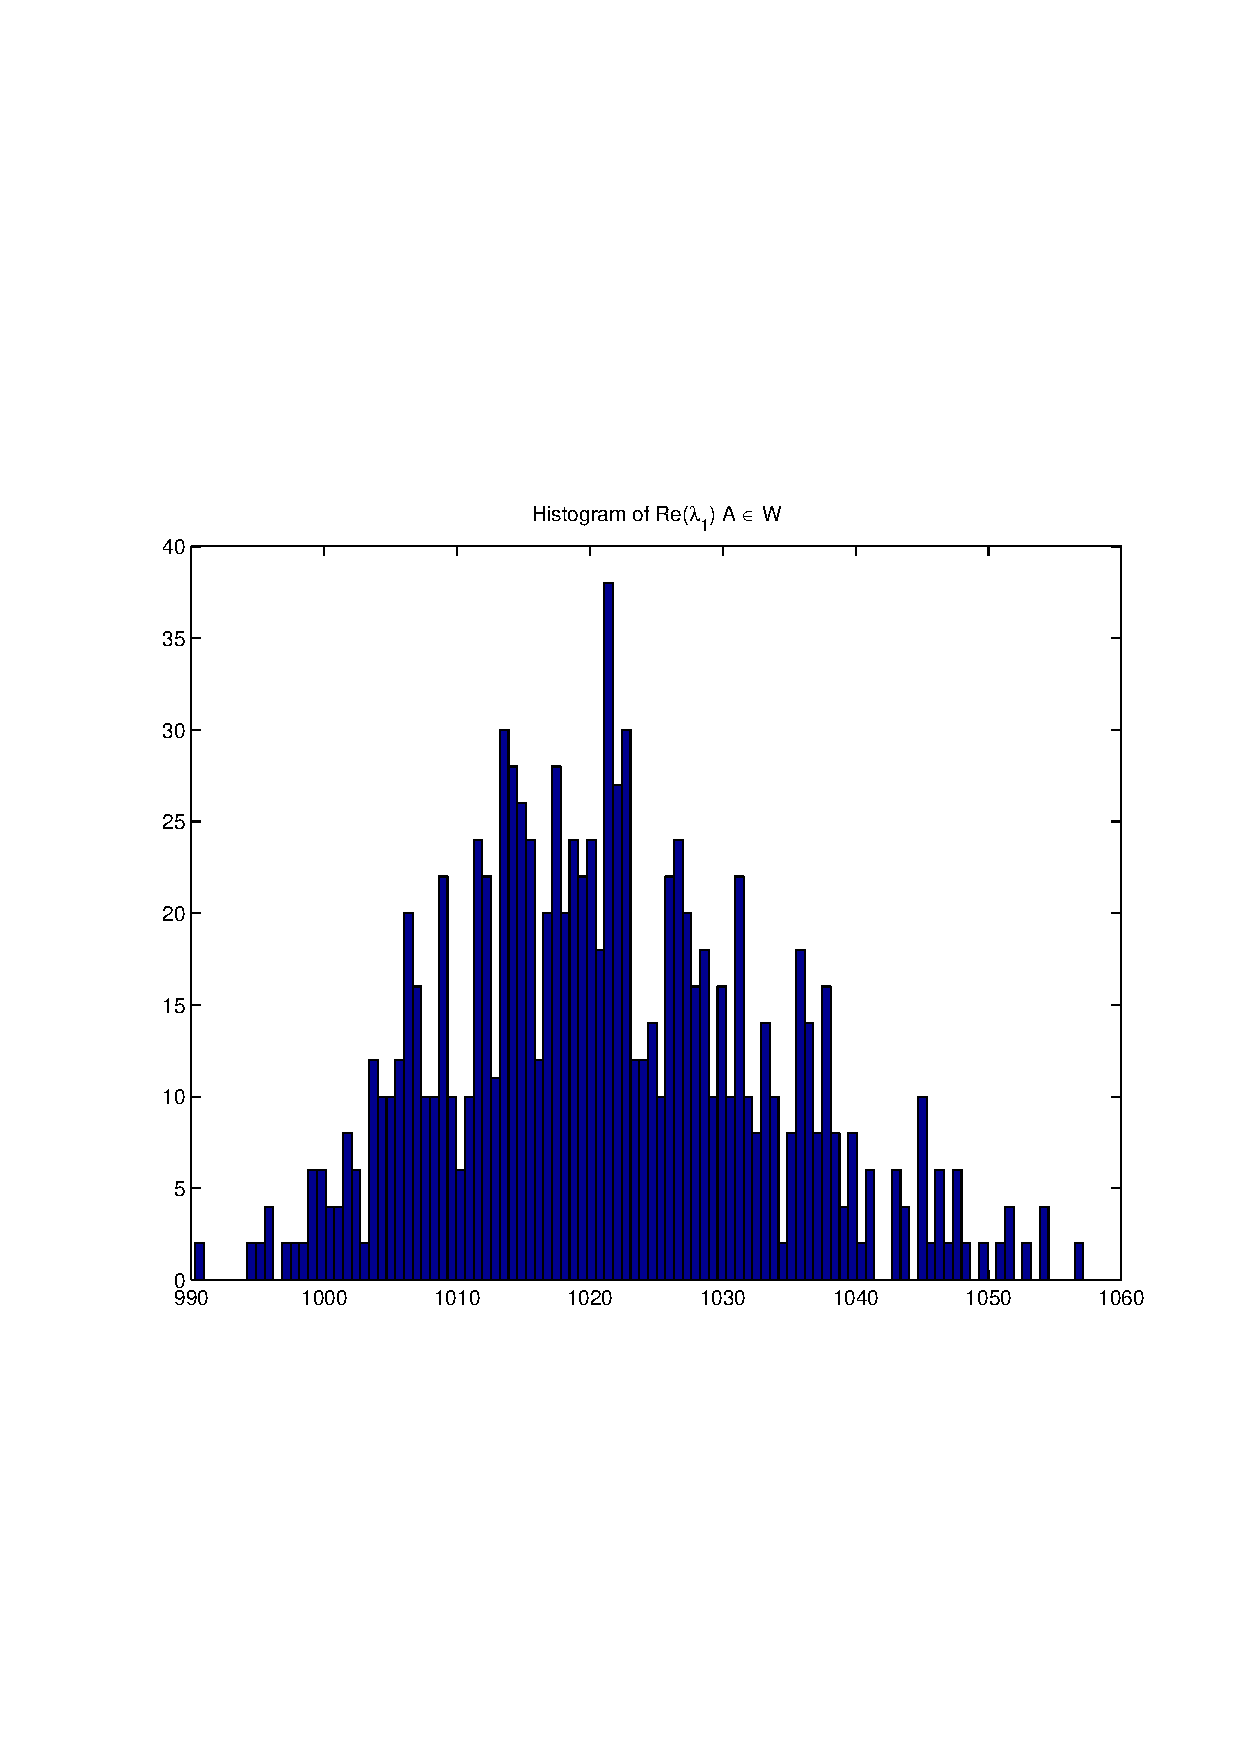
\includegraphics[width=10.0cm,height=10.0cm]{Re_TraceyWidom.pdf}

\includegraphics[width=10.0cm,height=10.0cm]{Im_TraceyWidom.pdf}

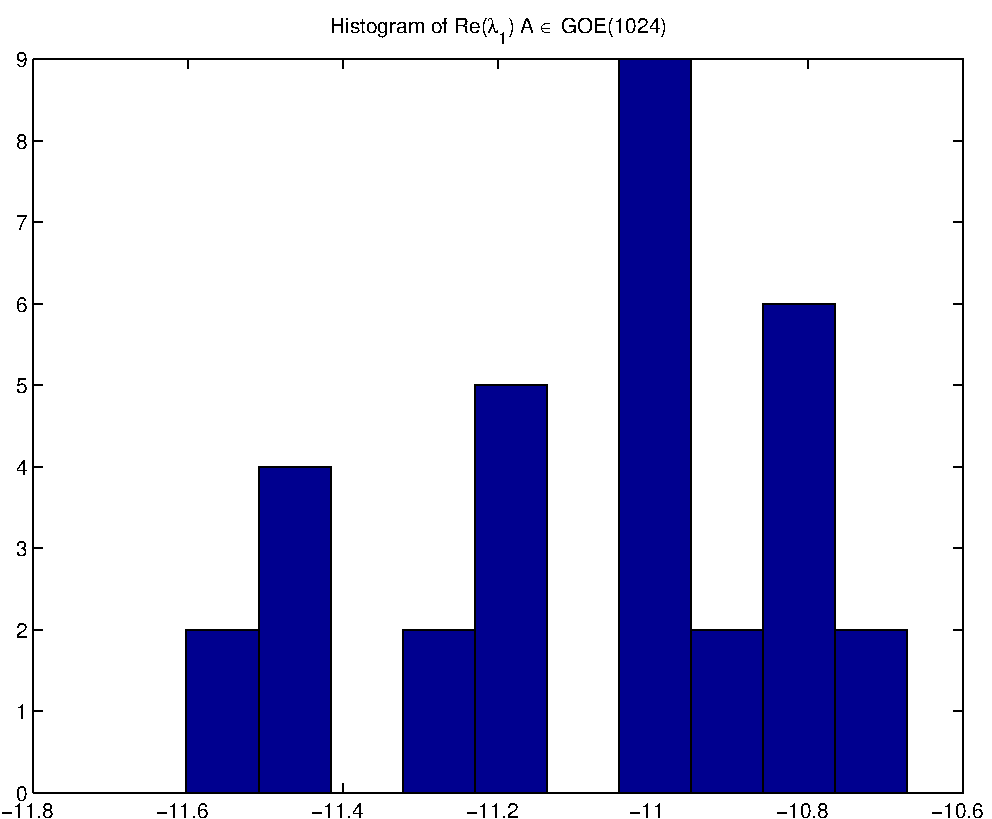
\includegraphics[width=10.0cm,height=10.0cm]{Re_Winger.pdf}

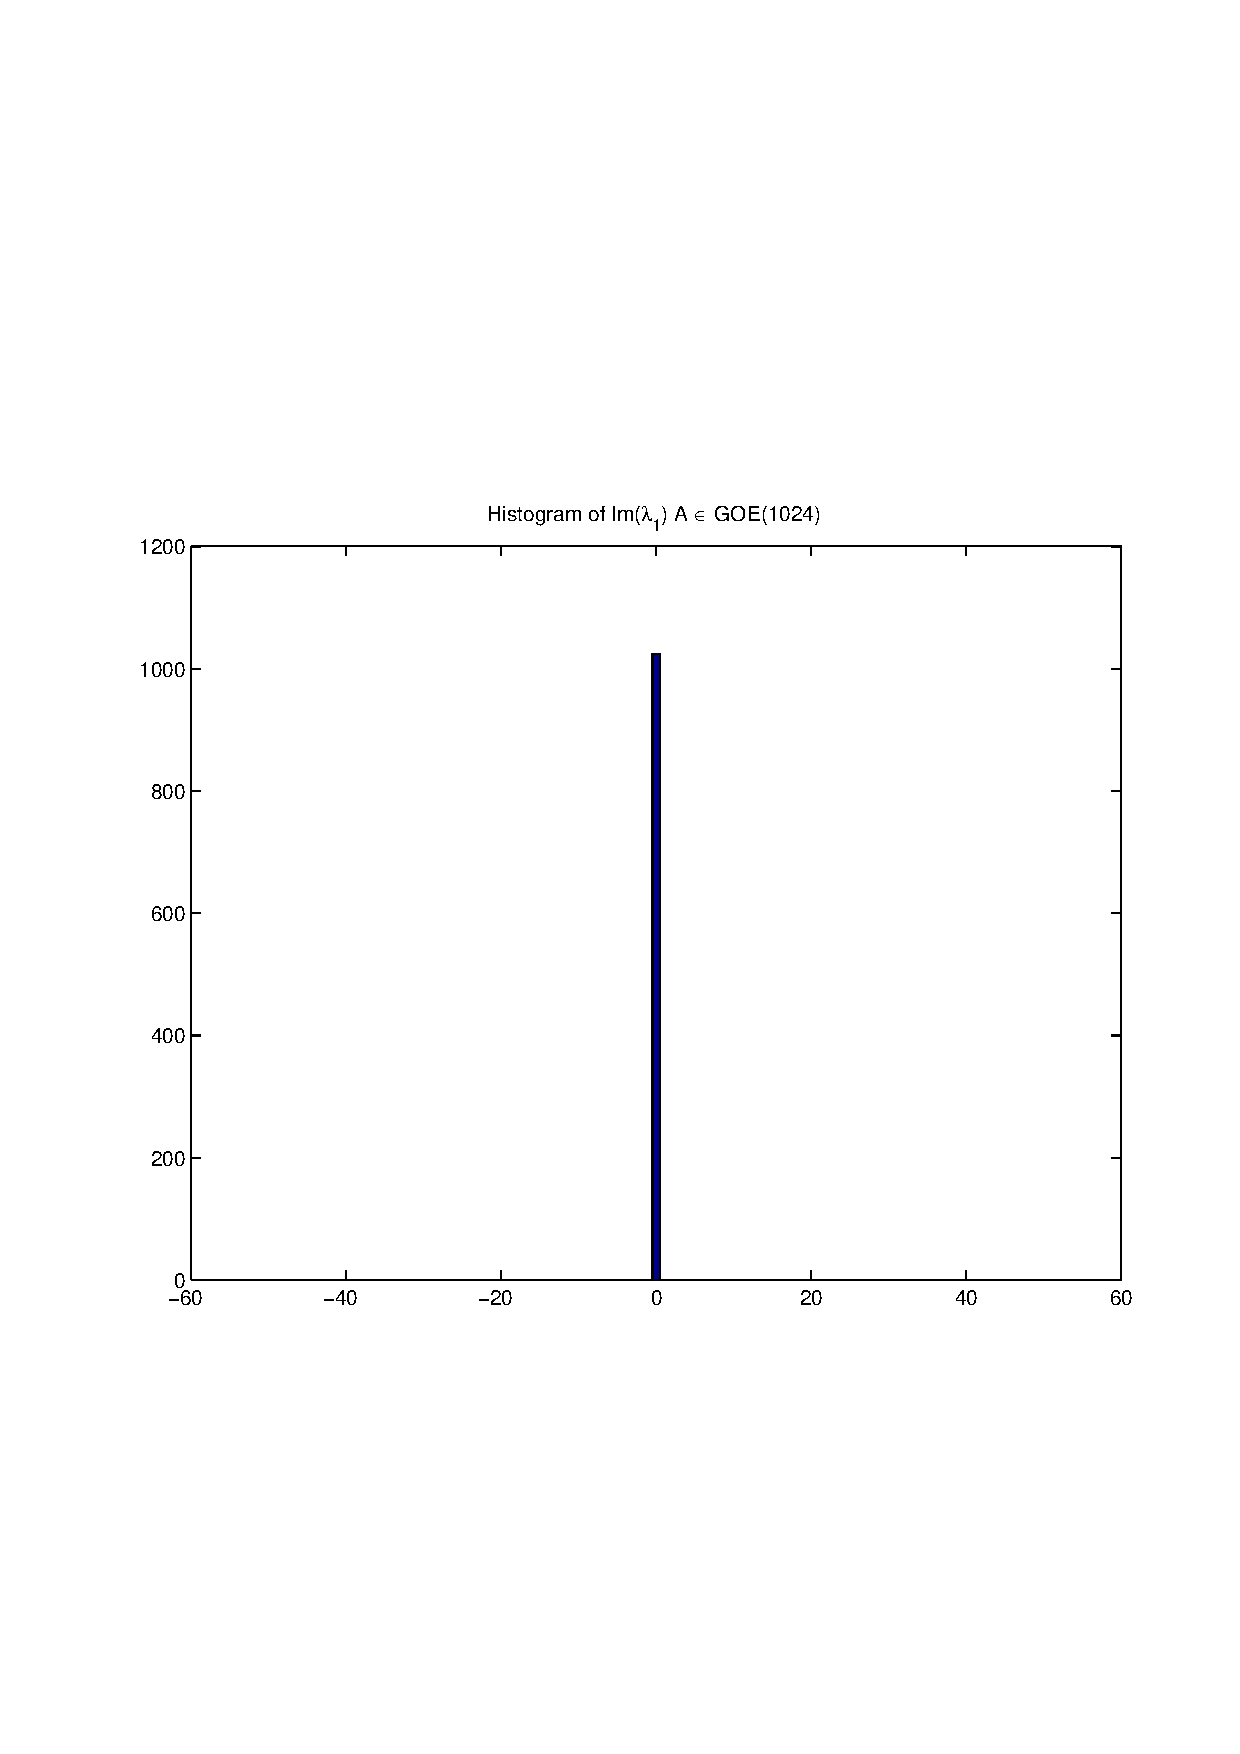
\includegraphics[width=10.0cm,height=10.0cm]{Im_Winger.pdf}

QueryPerformanceCounter  =  +8.860
\subsubsection{Approximate Winger Distribution}
\subsubsection{Verfy Winger Law.}
Let $M_n = [X_{ij} ]$ a symmetric n x n matrix with Random entries such that $X_{i,j} = X_{j,i}$, 		  and $X_{i,j}$ are iid $orall i < j,$ and $Xjj$ are iid $orall j  :  ; E[X^2_{ij} ] = 1, & E[X_{ij}] = 0$ 		  and that all moments exists for each of the entries.  		  The eigenvector of this random matrix; $ lambda_1 leq ... leq lambda_n$ depends continuously on $Mn$.
Dimension $n = +512$

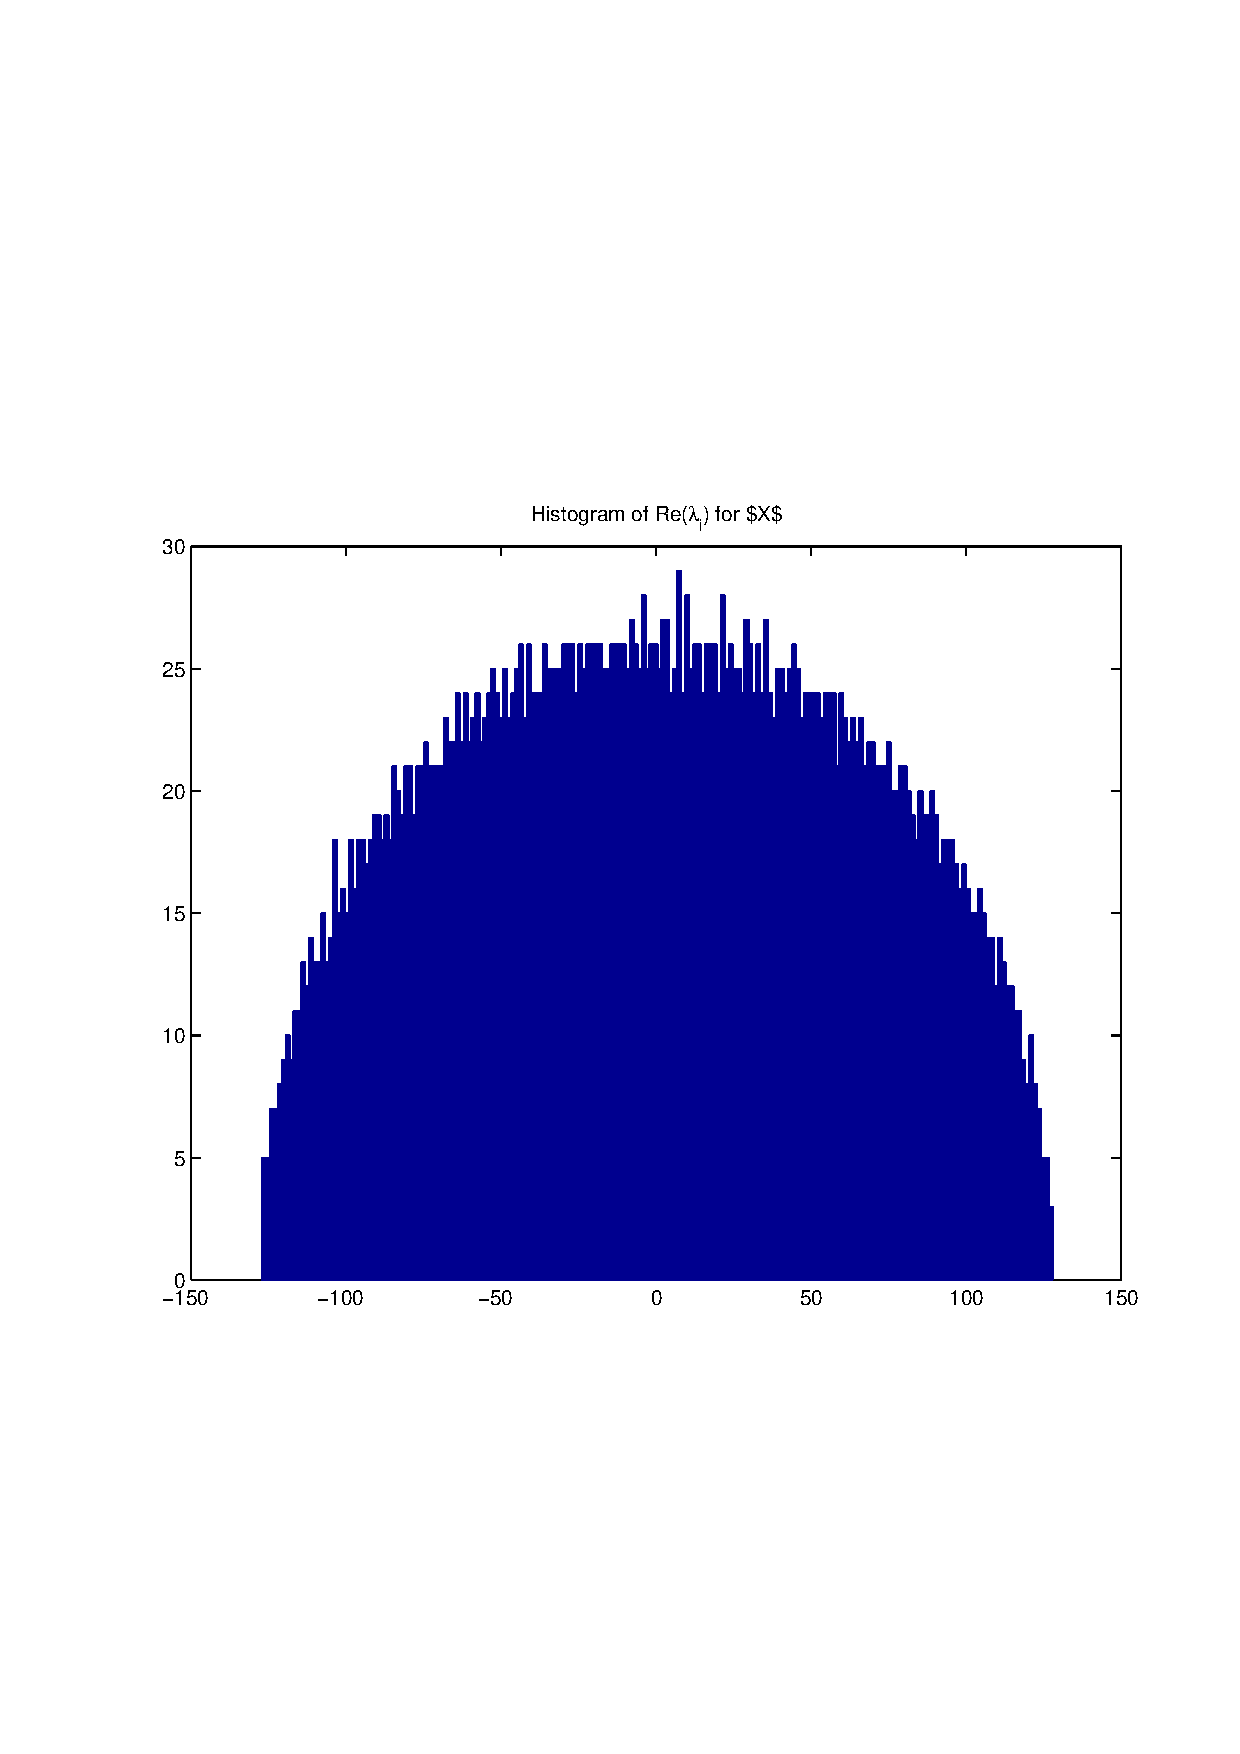
\includegraphics[width=10.0cm,height=10.0cm]{Re_lambda_n.pdf}

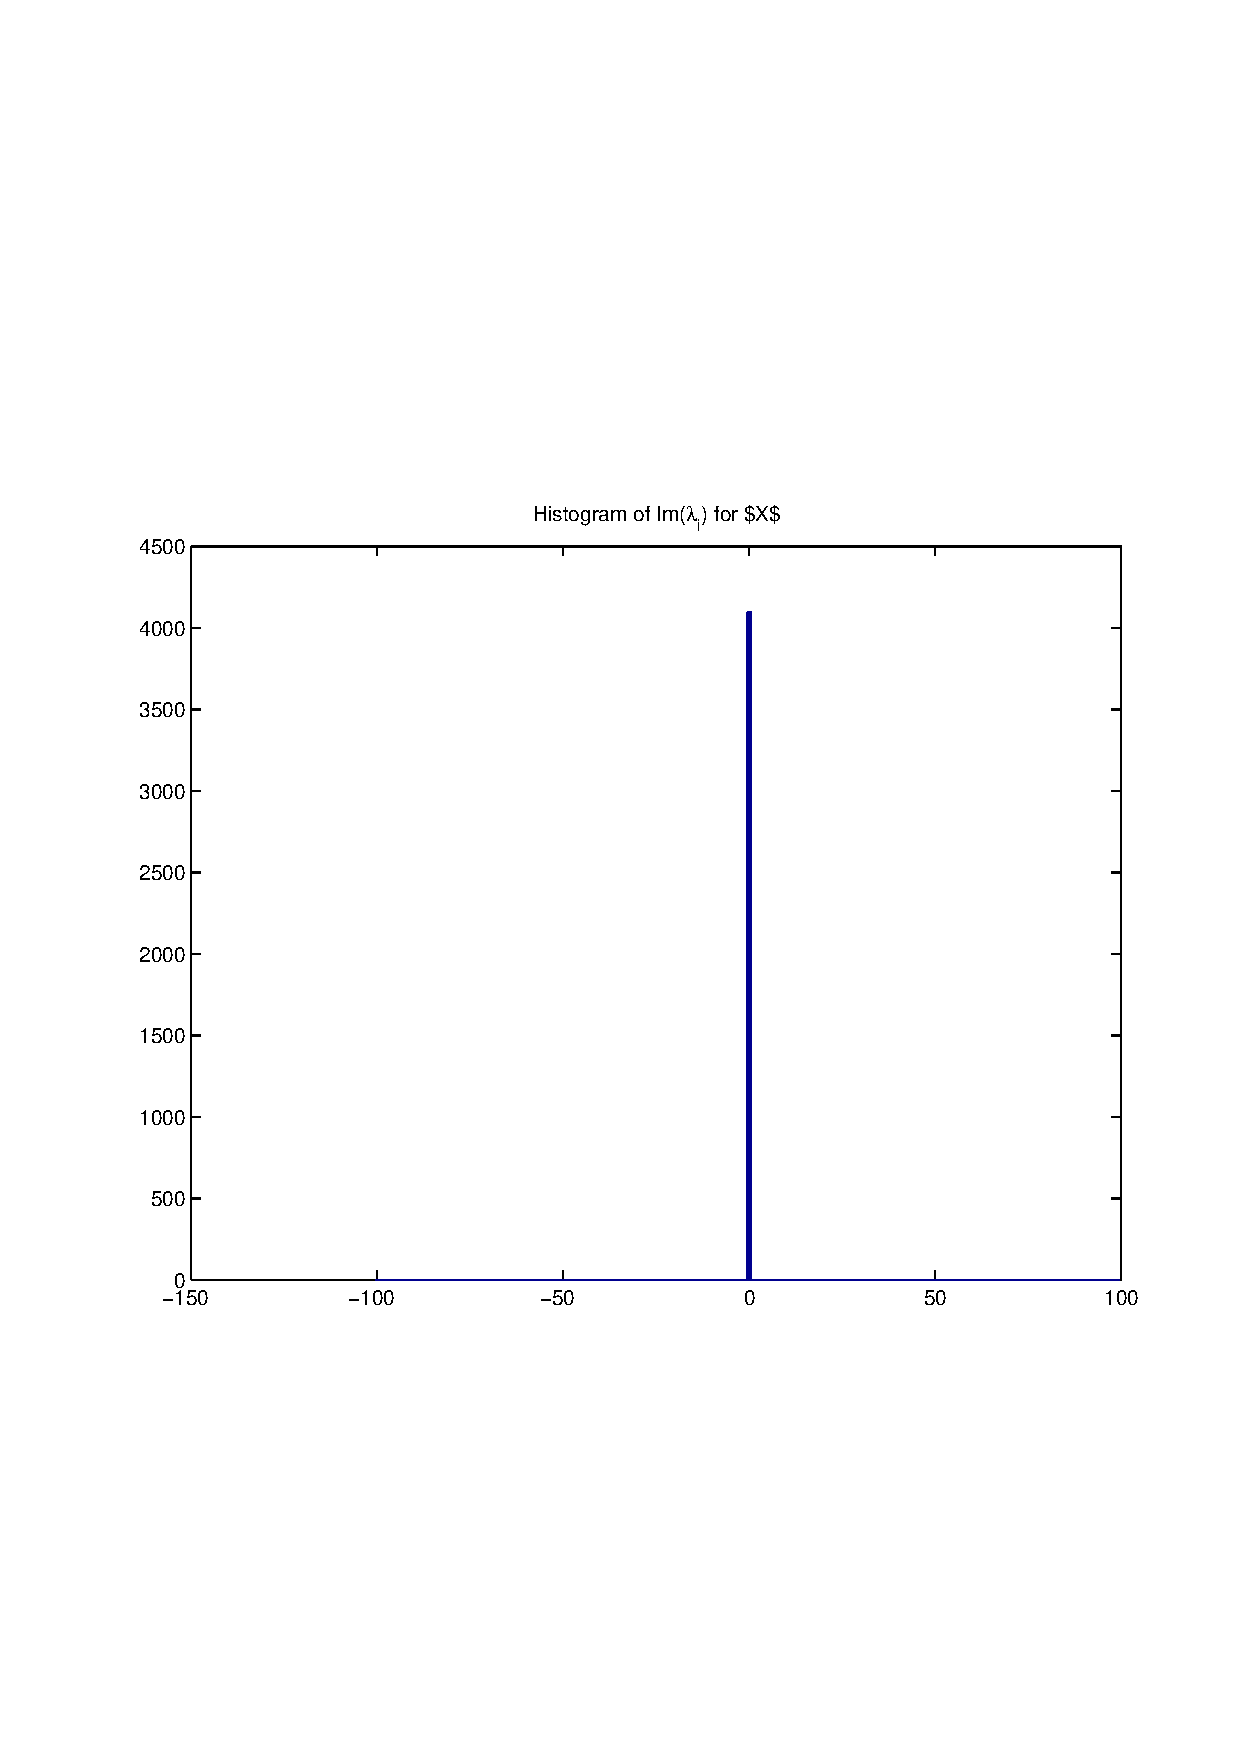
\includegraphics[width=10.0cm,height=10.0cm]{Im_lambda_n.pdf}

QueryPerformanceCounter  =  +2.725
\subsubsection{Matrix Exponential }
$SPD Matrix = \left(
\begin{array}{
cccccccc}
+10.539 & -0.499 & -0.010 & +0.368 & +0.465 & -0.492 & -0.126 & +0.437 \\
-0.499 & +7.286 & +0.365 & -0.481 & -0.337 & -0.466 & +0.279 & +0.056 \\
-0.010 & +0.365 & +6.705 & -0.205 & +0.467 & +0.131 & +0.077 & -0.089 \\
+0.368 & -0.481 & -0.205 & +6.496 & -0.402 & -0.209 & +0.043 & -0.041 \\
+0.465 & -0.337 & +0.467 & -0.402 & +4.578 & +0.272 & +0.289 & -0.285 \\
-0.492 & -0.466 & +0.131 & -0.209 & +0.272 & +8.181 & +0.343 & -0.244 \\
-0.126 & +0.279 & +0.077 & +0.043 & +0.289 & +0.343 & +5.938 & -0.212 \\
+0.437 & +0.056 & -0.089 & -0.041 & -0.285 & -0.244 & -0.212 & +9.691 \\
\end{array}
\right)$ \newline 

$SPD Eigs = \left(
\begin{array}{
cccccccc}
(+10.93611,+0.00000) & (+9.60778,+0.00000) & (+4.23666,+0.00000) & (+8.36911,+0.00000) & (+7.56229,+0.00000) & (+5.82791,+0.00000) & (+6.54198,+0.00000) & (+6.33139,+0.00000) \\
\end{array}
\right)$ \newline 

$exp(SPD) = \left(
\begin{array}{
cccccccc}
+47863.969 & -6460.093 & -1078.770 & +4706.958 & +2535.224 & -8475.398 & -2406.368 & +12977.552 \\
-6460.093 & +2780.574 & +516.920 & -1069.918 & -548.083 & -109.707 & +386.466 & -807.216 \\
-1078.770 & +516.920 & +1015.281 & -385.755 & +176.069 & +458.541 & +212.284 & -859.022 \\
+4706.958 & -1069.918 & -385.755 & +1267.210 & +111.181 & -1018.272 & -287.809 & +1036.628 \\
+2535.224 & -548.083 & +176.069 & +111.181 & +413.265 & +135.193 & +45.490 & -502.411 \\
-8475.398 & -109.707 & +458.541 & -1018.272 & +135.193 & +5613.026 & +968.003 & -4270.737 \\
-2406.368 & +386.466 & +212.284 & -287.809 & +45.490 & +968.003 & +632.432 & -1645.725 \\
+12977.552 & -807.216 & -859.022 & +1036.628 & -502.411 & -4270.737 & -1645.725 & +19362.944 \\
\end{array}
\right)$ \newline 

$exp(SPD) eigs = \left(
\begin{array}{
cccccccc}
(+56168.17045,+0.00000) & (+14880.07985,+0.00000) & (+4311.77579,+0.00000) & (+1924.25027,+0.00000) & (+69.17669,+0.00000) & (+339.64809,+0.00000) & (+693.66208,+0.00000) & (+561.93669,+0.00000) \\
\end{array}
\right)$ \newline 

$log(exp(SPD) eigs)  = \left(
\begin{array}{
cccccccc}
(+10.93611,+0.00000) & (+9.60778,+0.00000) & (+8.36911,+0.00000) & (+7.56229,+0.00000) & (+4.23666,+0.00000) & (+5.82791,+0.00000) & (+6.54198,+0.00000) & (+6.33139,+0.00000) \\
\end{array}
\right)$ \newline 

$exp(Id) = \left(
\begin{array}{
cccccccc}
+2.718 & +0.000 & +0.000 & +0.000 & +0.000 & +0.000 & +0.000 & +0.000 \\
+0.000 & +2.718 & +0.000 & +0.000 & +0.000 & +0.000 & +0.000 & +0.000 \\
+0.000 & +0.000 & +2.718 & +0.000 & +0.000 & +0.000 & +0.000 & +0.000 \\
+0.000 & +0.000 & +0.000 & +2.718 & +0.000 & +0.000 & +0.000 & +0.000 \\
+0.000 & +0.000 & +0.000 & +0.000 & +2.718 & +0.000 & +0.000 & +0.000 \\
+0.000 & +0.000 & +0.000 & +0.000 & +0.000 & +2.718 & +0.000 & +0.000 \\
+0.000 & +0.000 & +0.000 & +0.000 & +0.000 & +0.000 & +2.718 & +0.000 \\
+0.000 & +0.000 & +0.000 & +0.000 & +0.000 & +0.000 & +0.000 & +2.718 \\
\end{array}
\right)$ \newline 

$exp(Id) eigs = \left(
\begin{array}{
cccccccc}
(+2.71828,+0.00000) & (+2.71828,+0.00000) & (+2.71828,+0.00000) & (+2.71828,+0.00000) & (+2.71828,+0.00000) & (+2.71828,+0.00000) & (+2.71828,+0.00000) & (+2.71828,+0.00000) \\
\end{array}
\right)$ \newline 

$log(exp(Id) eigs)  = \left(
\begin{array}{
cccccccc}
(+1.00000,+0.00000) & (+1.00000,+0.00000) & (+1.00000,+0.00000) & (+1.00000,+0.00000) & (+1.00000,+0.00000) & (+1.00000,+0.00000) & (+1.00000,+0.00000) & (+1.00000,+0.00000) \\
\end{array}
\right)$ \newline 

For $n  \in  \dblz [16,128)$ we calculate  $|( SPD(n) Eigs - log(exp(SPD(n)) eigs)|_{l^2}$

$|( SPD(n) Eigs - log(exp(SPD(n)) eigs)|_{l^2} = \left(
\begin{array}{
cccccccccccccccccccccccccccccccccccccccccccccccccccccccccccccccccccccccccccccccccccccccccccccccccccccccccccccccc}
(+5.36543,+0.00000) & (+5.36543,+0.00000) & (+5.36543,+0.00000) & (+5.36543,+0.00000) & (+5.36543,+0.00000) & (+5.36543,+0.00000) & (+5.36543,+0.00000) & (+5.36543,+0.00000) & (+5.36543,+0.00000) & (+5.36543,+0.00000) & (+5.36543,+0.00000) & (+5.36543,+0.00000) & (+5.36543,+0.00000) & (+5.36543,+0.00000) & (+5.36543,+0.00000) & (+5.36543,+0.00000) & (+5.36543,+0.00000) & (+5.36543,+0.00000) & (+5.36543,+0.00000) & (+5.36543,+0.00000) & (+5.36543,+0.00000) & (+5.36543,+0.00000) & (+5.36543,+0.00000) & (+5.36543,+0.00000) & (+5.36543,+0.00000) & (+5.36543,+0.00000) & (+5.36543,+0.00000) & (+5.36543,+0.00000) & (+5.36543,+0.00000) & (+5.36543,+0.00000) & (+5.36543,+0.00000) & (+5.36543,+0.00000) & (+5.36543,+0.00000) & (+5.36543,+0.00000) & (+5.36543,+0.00000) & (+5.36543,+0.00000) & (+5.36543,+0.00000) & (+5.36543,+0.00000) & (+5.36543,+0.00000) & (+5.36543,+0.00000) & (+5.36543,+0.00000) & (+5.36543,+0.00000) & (+5.36543,+0.00000) & (+5.36543,+0.00000) & (+5.36543,+0.00000) & (+5.36543,+0.00000) & (+5.36543,+0.00000) & (+5.36543,+0.00000) & (+0.00000,+0.00000) & (+0.00000,+0.00000) & (+0.00000,+0.00000) & (+0.00000,+0.00000) & (+0.00000,+0.00000) & (+0.00000,+0.00000) & (+0.00000,+0.00000) & (+0.00000,+0.00000) & (+0.00000,+0.00000) & (+0.00000,+0.00000) & (+0.00000,+0.00000) & (+0.00000,+0.00000) & (+0.00000,+0.00000) & (+0.00000,+0.00000) & (+0.00000,+0.00000) & (+0.00000,+0.00000) & (+0.00000,+0.00000) & (+0.00000,+0.00000) & (+0.00000,+0.00000) & (+0.00000,+0.00000) & (+0.00000,+0.00000) & (+0.00000,+0.00000) & (+0.00000,+0.00000) & (+0.00000,+0.00000) & (+0.00000,+0.00000) & (+0.00000,+0.00000) & (+0.00000,+0.00000) & (+0.00000,+0.00000) & (+0.00000,+0.00000) & (+0.00000,+0.00000) & (+0.00000,+0.00000) & (+0.00000,+0.00000) & (+0.00000,+0.00000) & (+0.00000,+0.00000) & (+0.00000,+0.00000) & (+0.00000,+0.00000) & (+0.00000,+0.00000) & (+0.00000,+0.00000) & (+0.00000,+0.00000) & (+0.00000,+0.00000) & (+0.00000,+0.00000) & (+0.00000,+0.00000) & (+0.00000,+0.00000) & (+0.00000,+0.00000) & (+0.00000,+0.00000) & (+0.00000,+0.00000) & (+0.00000,+0.00000) & (+0.00000,+0.00000) & (+0.00000,+0.00000) & (+0.00000,+0.00000) & (+0.00000,+0.00000) & (+0.00000,+0.00000) & (+0.00000,+0.00000) & (+0.00000,+0.00000) & (+0.00000,+0.00000) & (+0.00000,+0.00000) & (+0.00000,+0.00000) & (+0.00000,+0.00000) & (+0.00000,+0.00000) & (+0.00000,+0.00000) & (+0.00000,+0.00000) & (+0.00000,+0.00000) & (+0.00000,+0.00000) & (+0.00000,+0.00000) \\
\end{array}
\right)$ \newline 

QueryPerformanceCounter  =  +0.04861
The sample size generated for this run is 100000.

\newpage
uniform \begin{tabular}{|c|c|c|c|}  mean & variance & skewness & kurtosis \\  \hline
$\mu_1 = +0.50030$ & $\mu_2 = +0.08353$ & $\mu_3 = +0.00339$ & $\mu_4 =+1.80113$ \\
\end{tabular}

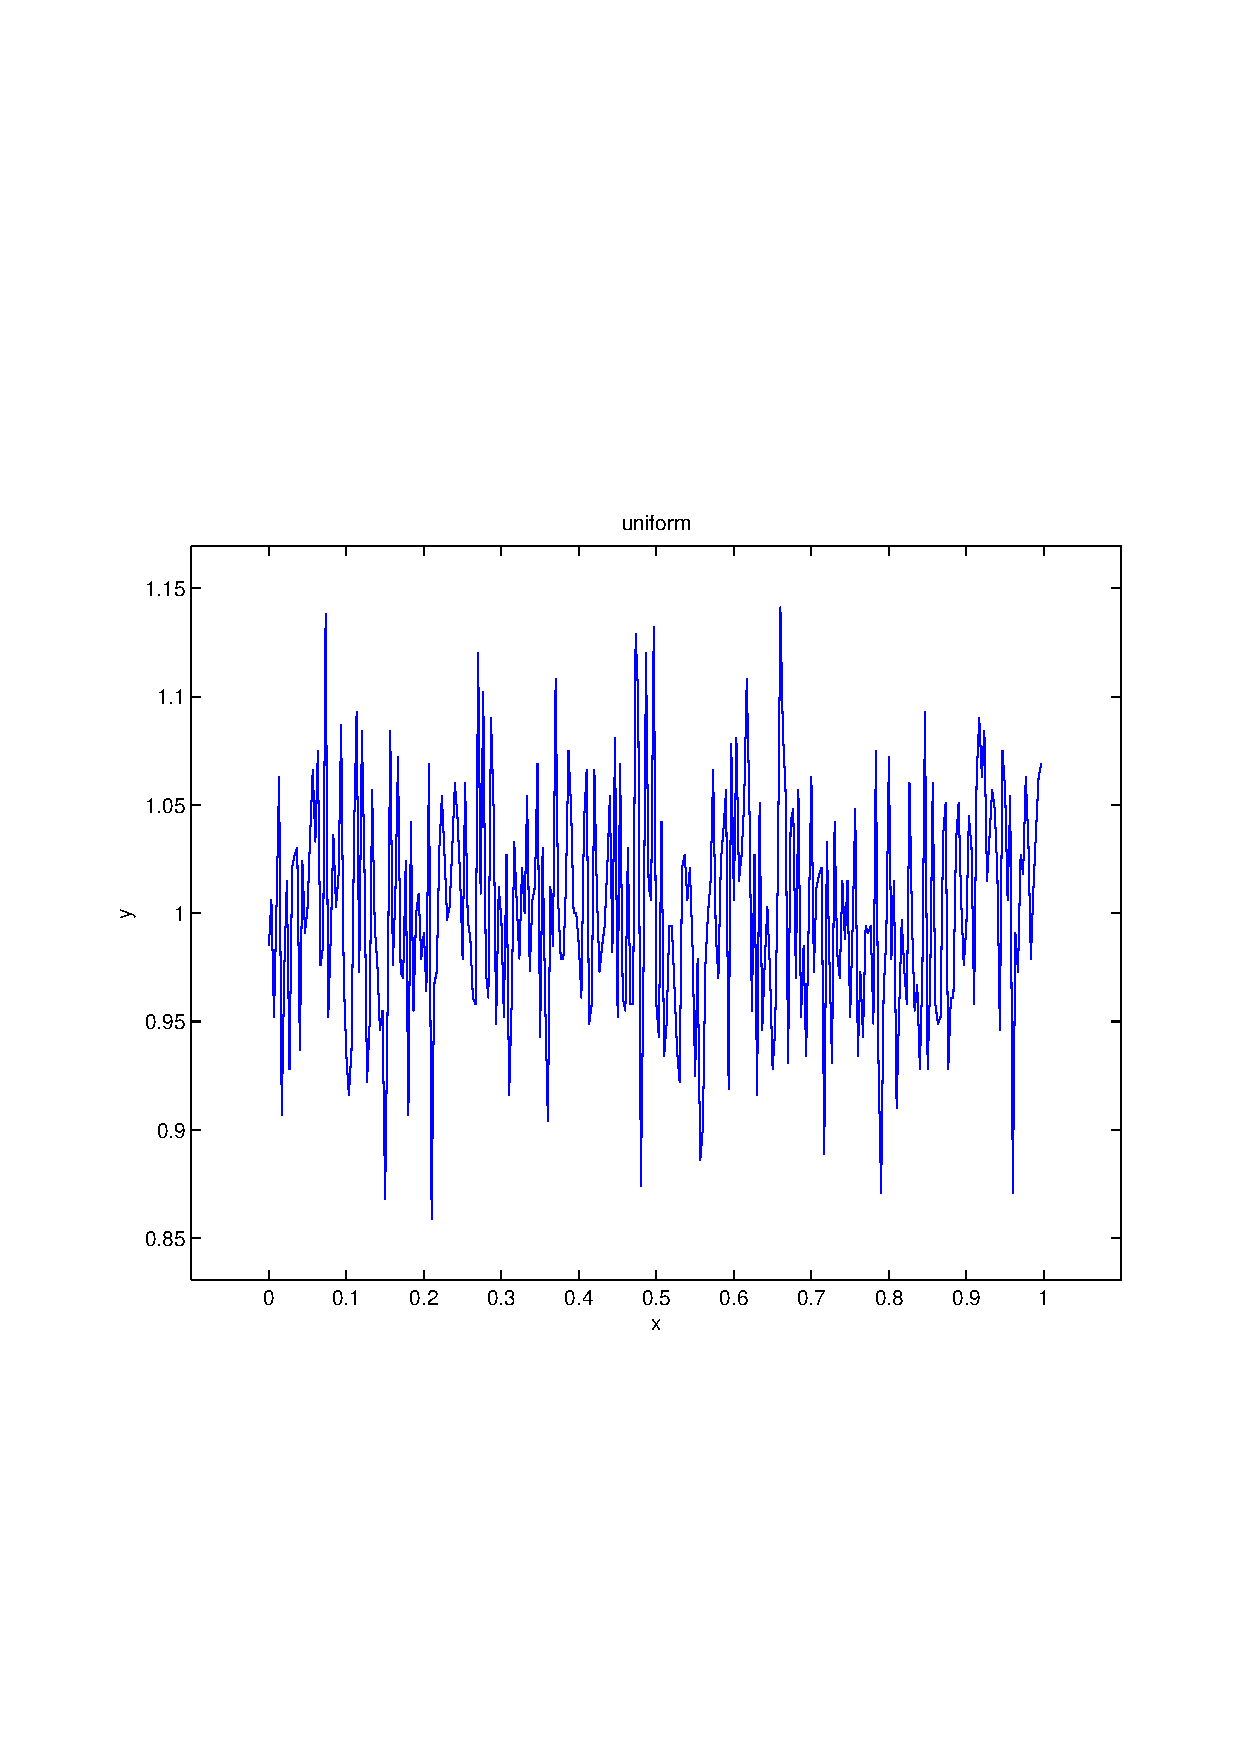
\includegraphics[width=5cm,height=5cm]{uniform.pdf}

cauchy \begin{tabular}{|c|c|c|c|}  mean & variance & skewness & kurtosis \\  \hline
$\mu_1 = +0.44288$ & $\mu_2 = +0.05341$ & $\mu_3 = +0.63935$ & $\mu_4 =+3.28094$ \\
\end{tabular}

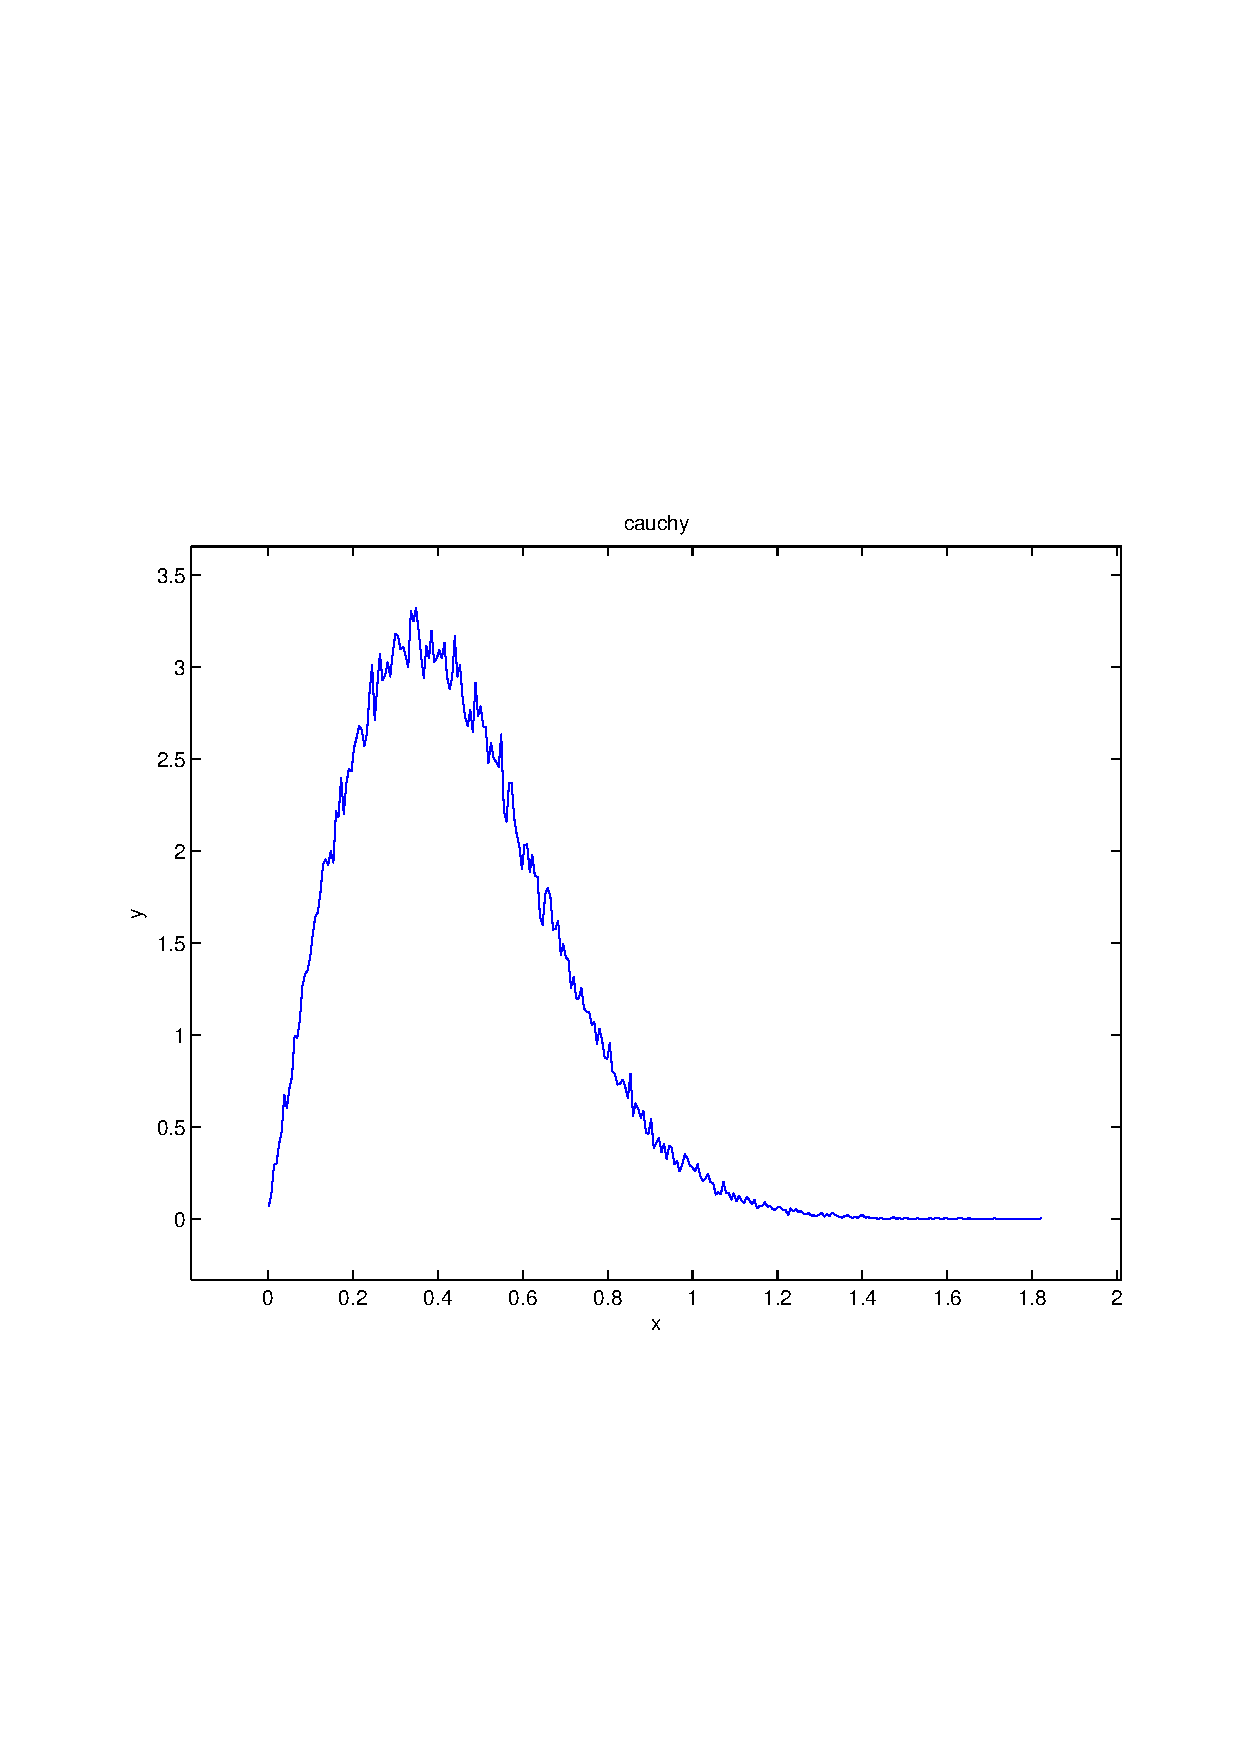
\includegraphics[width=5cm,height=5cm]{cauchy.pdf}

exponential \begin{tabular}{|c|c|c|c|}  mean & variance & skewness & kurtosis \\  \hline
$\mu_1 = +1.99647$ & $\mu_2 = +3.99339$ & $\mu_3 = +2.03097$ & $\mu_4 =+9.30842$ \\
\end{tabular}

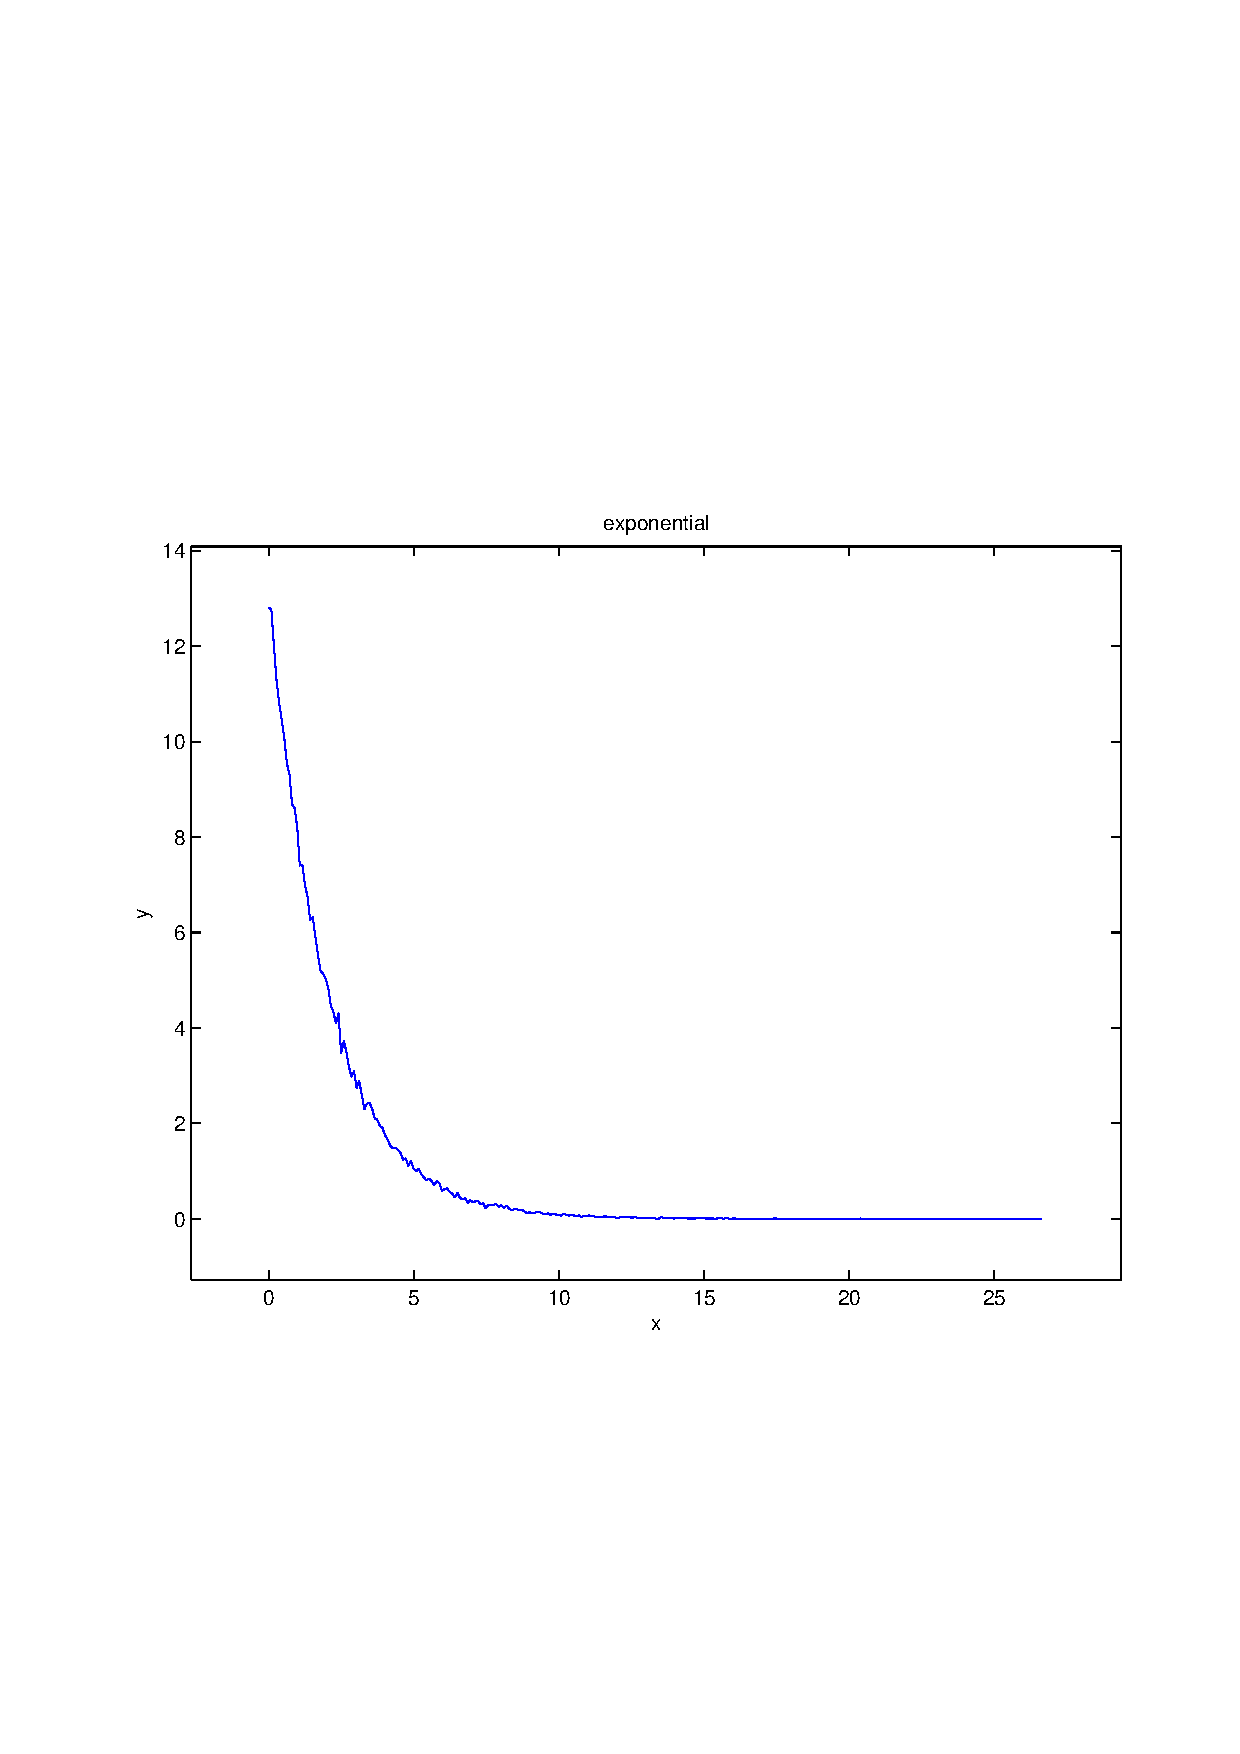
\includegraphics[width=5cm,height=5cm]{exponential.pdf}

\newpage
gamma \begin{tabular}{|c|c|c|c|}  mean & variance & skewness & kurtosis \\  \hline
$\mu_1 = +1.89423$ & $\mu_2 = +1.90511$ & $\mu_3 = +1.47668$ & $\mu_4 =+6.29196$ \\
\end{tabular}

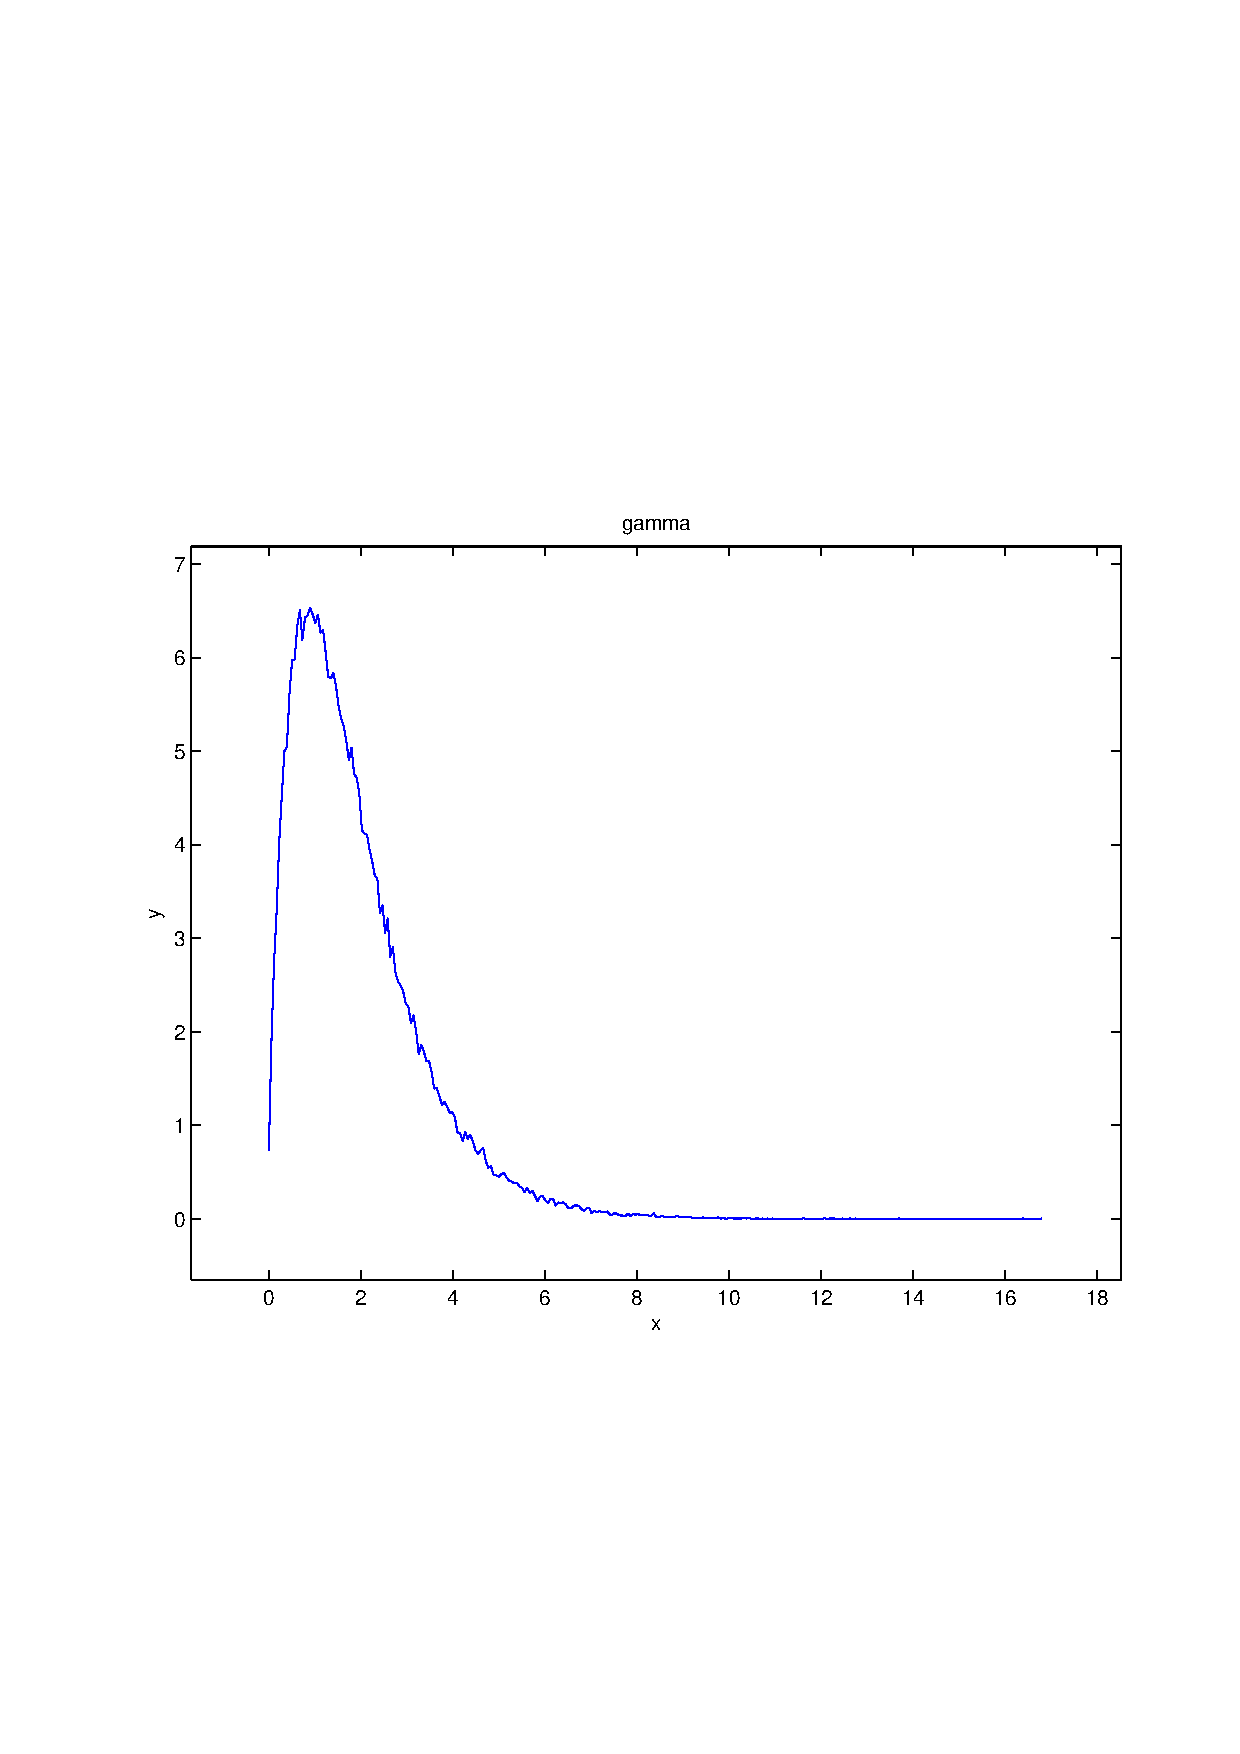
\includegraphics[width=5cm,height=5cm]{gamma.pdf}

GIG \begin{tabular}{|c|c|c|c|}  mean & variance & skewness & kurtosis \\  \hline
$\mu_1 = +0.80934$ & $\mu_2 = +11.17234$ & $\mu_3 = +14.68669$ & $\mu_4 =+286.91260$ \\
\end{tabular}

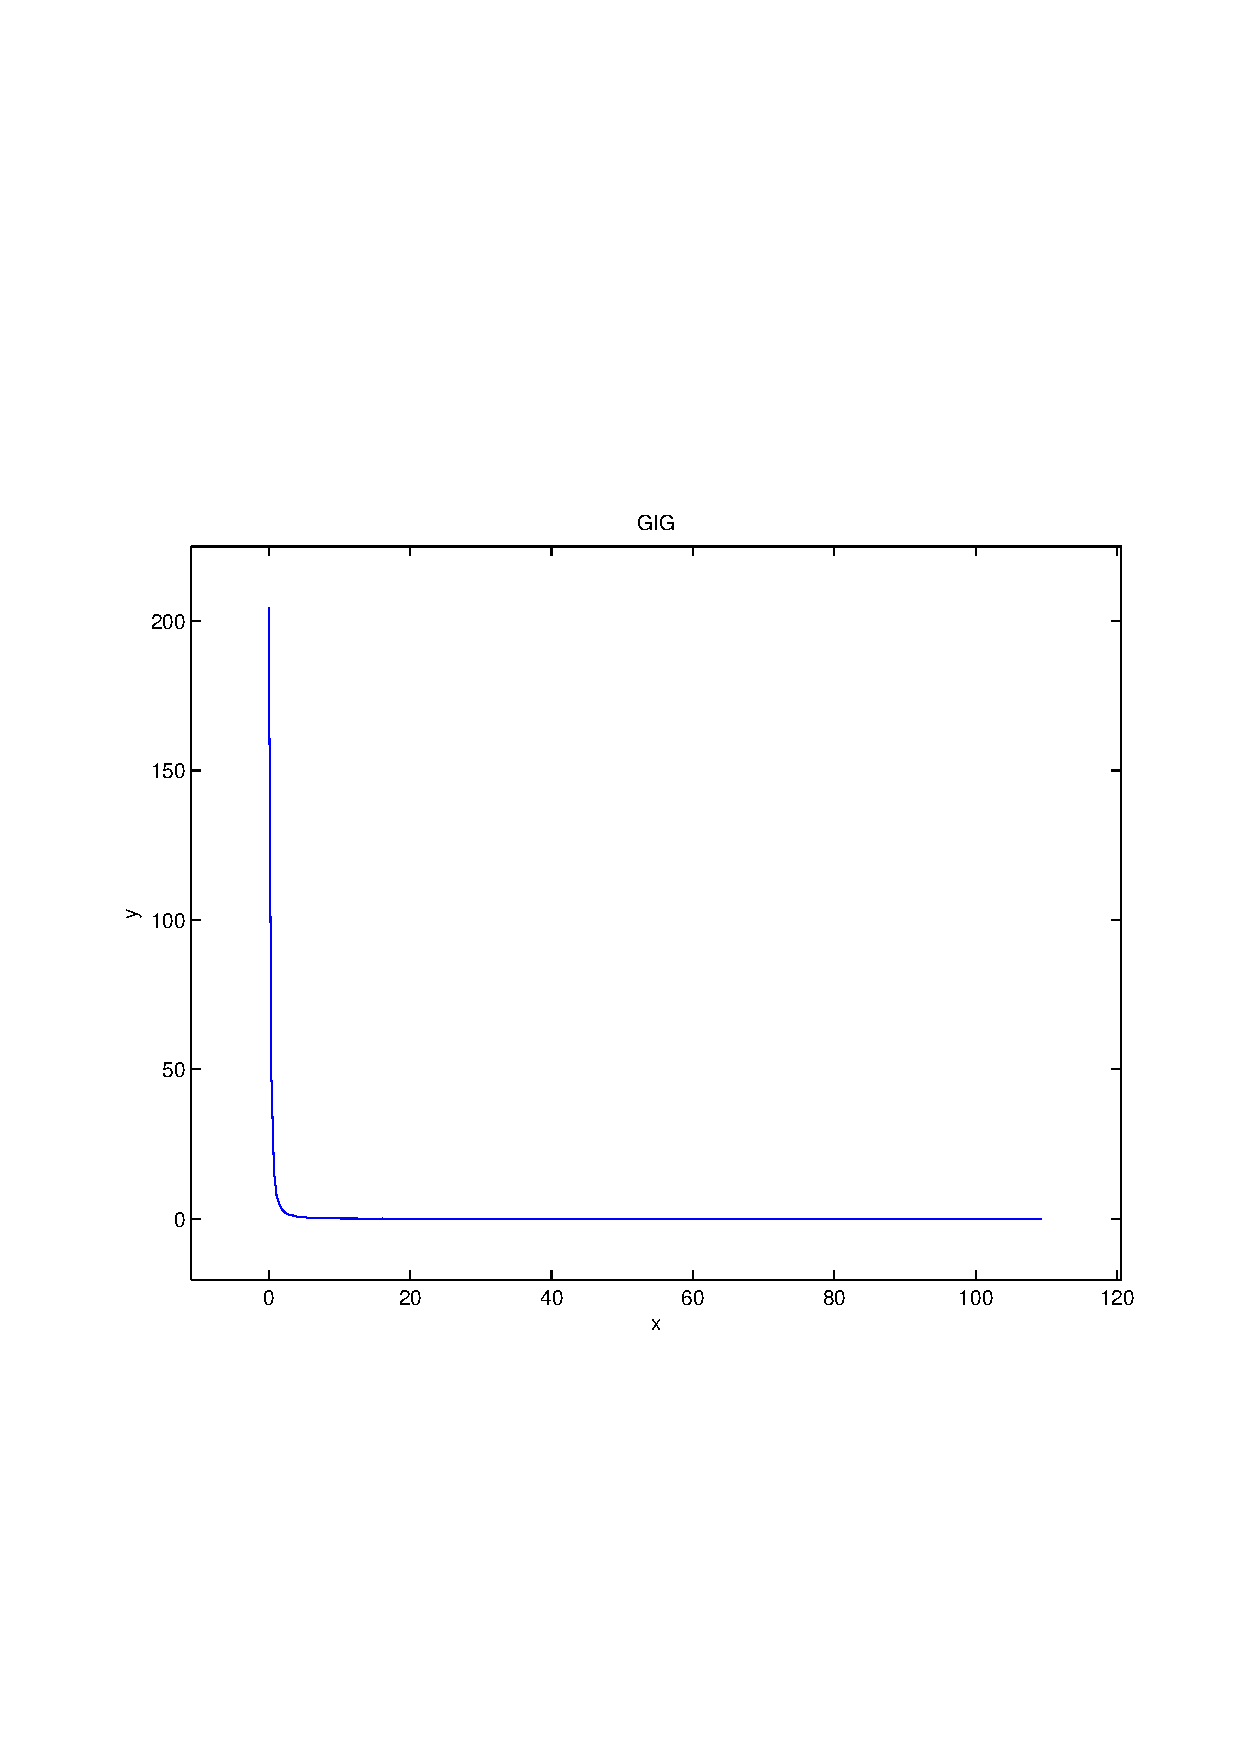
\includegraphics[width=5cm,height=5cm]{GIG.pdf}

normal-box-muller \begin{tabular}{|c|c|c|c|}  mean & variance & skewness & kurtosis \\  \hline
$\mu_1 = -0.00236$ & $\mu_2 = +1.00105$ & $\mu_3 = +0.00728$ & $\mu_4 =+3.03325$ \\
\end{tabular}

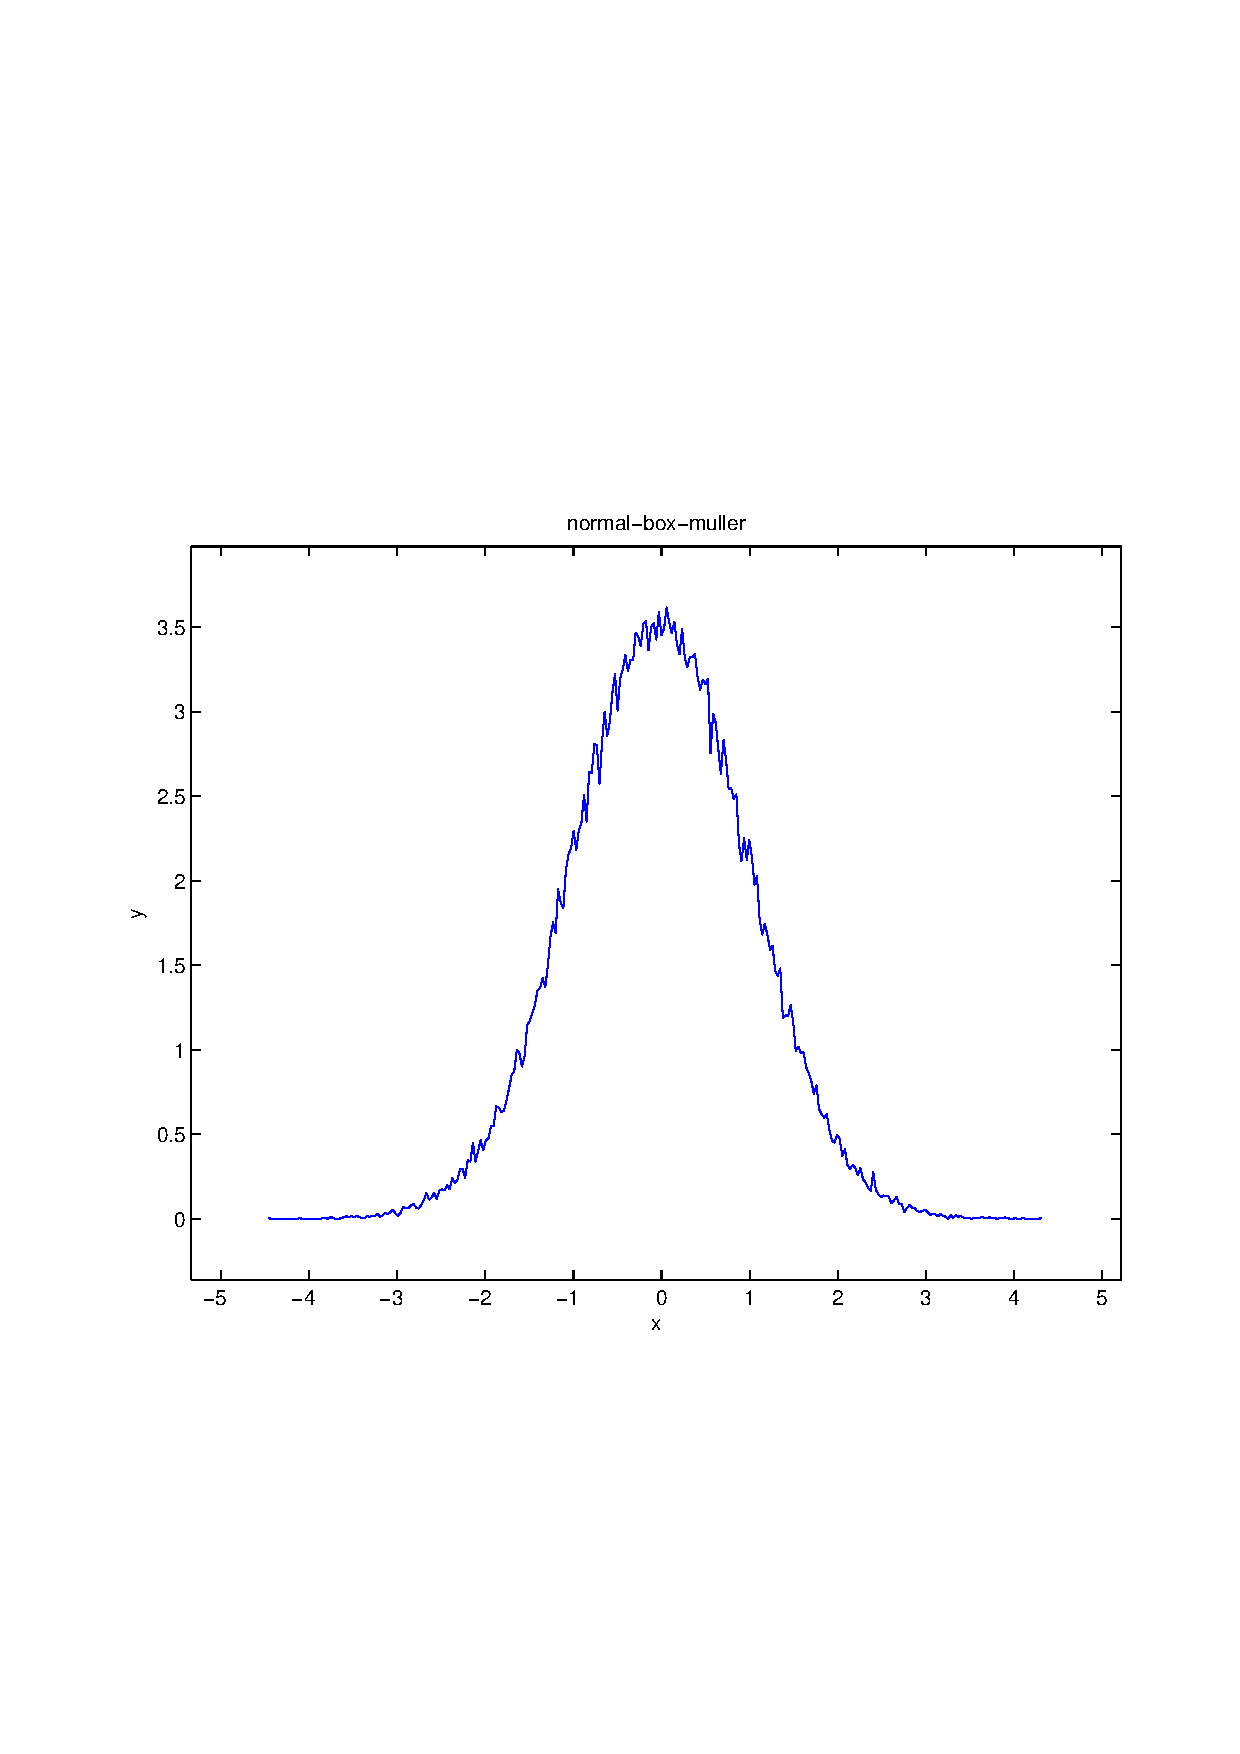
\includegraphics[width=5cm,height=5cm]{normal-box-muller.pdf}

\newpage
normal-inverse-approximation \begin{tabular}{|c|c|c|c|}  mean & variance & skewness & kurtosis \\  \hline
$\mu_1 = +0.00230$ & $\mu_2 = +1.00486$ & $\mu_3 = +0.01163$ & $\mu_4 =+2.99254$ \\
\end{tabular}

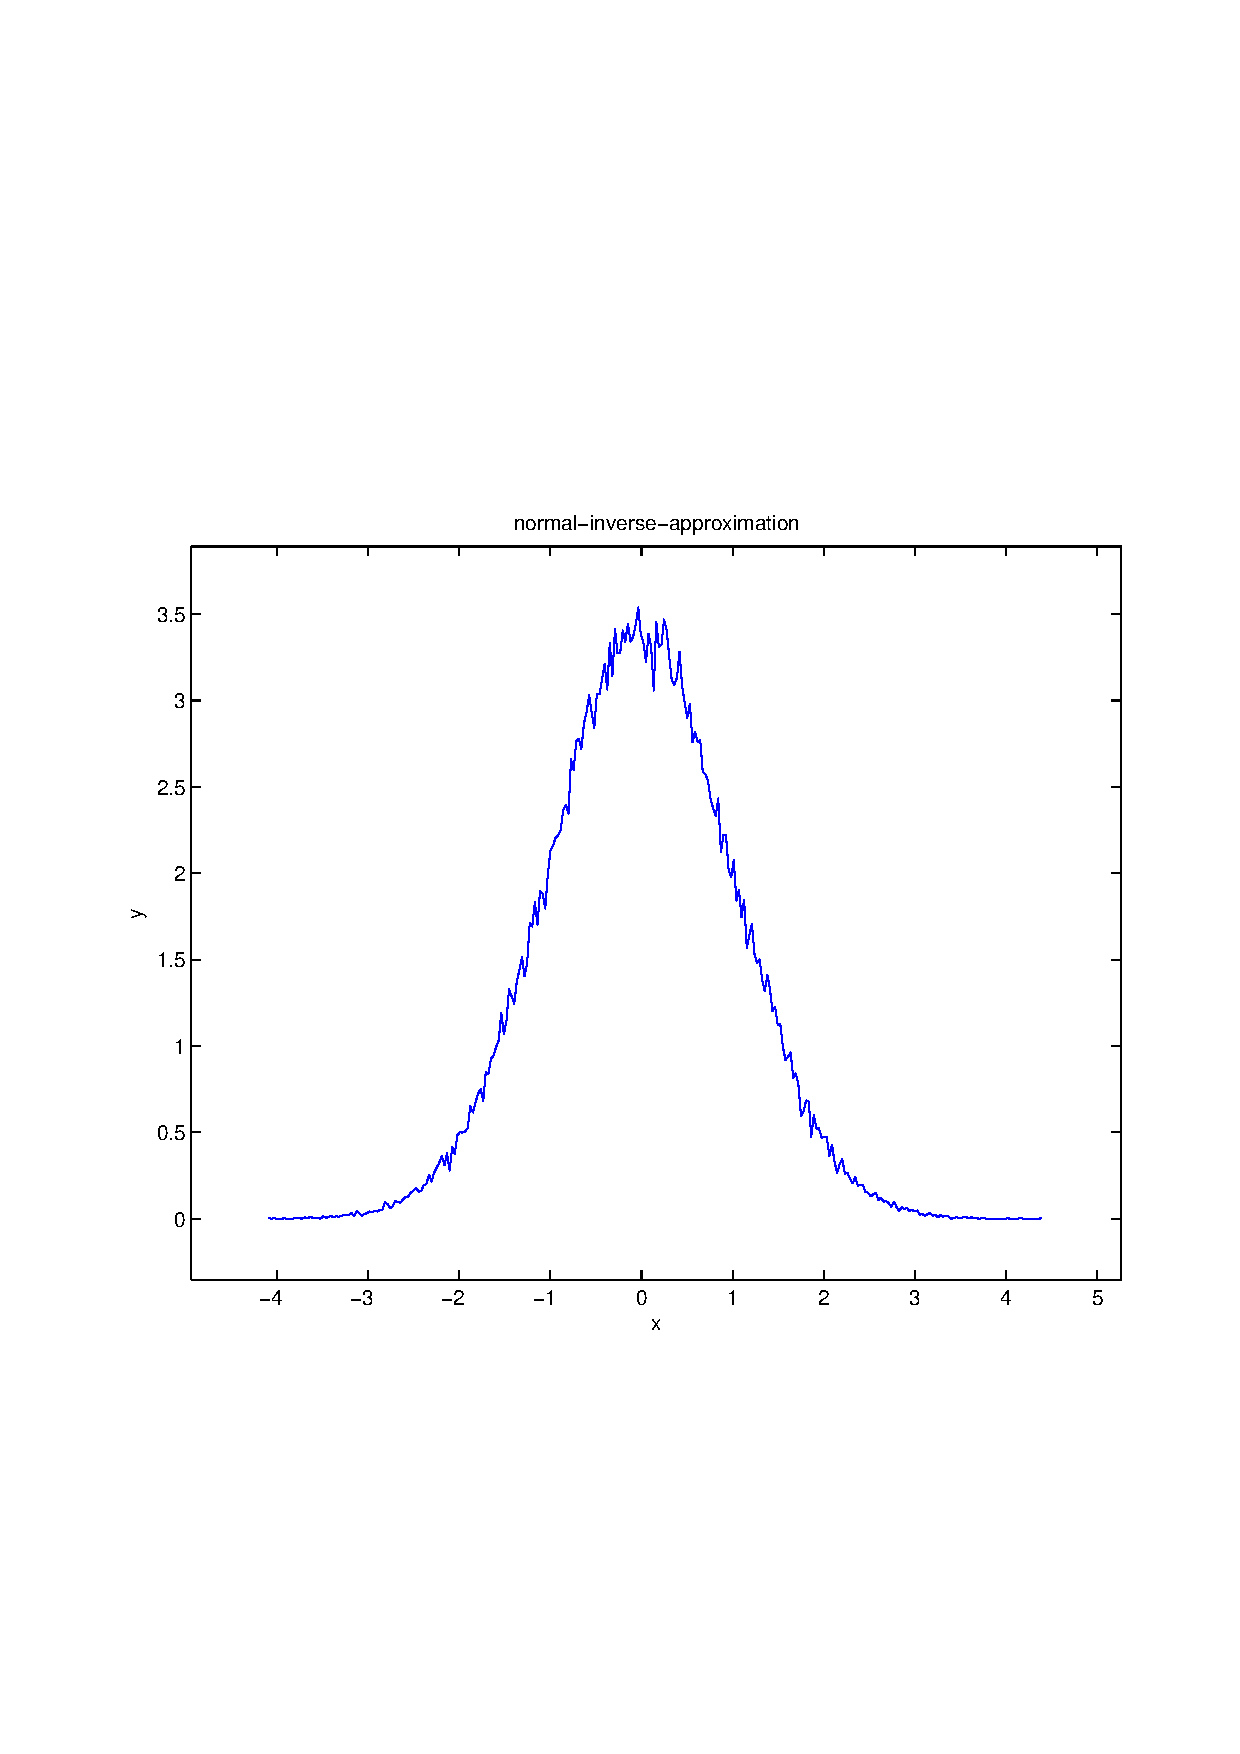
\includegraphics[width=5cm,height=5cm]{normal-inverse-approximation.pdf}

pareto \begin{tabular}{|c|c|c|c|}  mean & variance & skewness & kurtosis \\  \hline
$\mu_1 = +3184578.26493$ & $\mu_2 = +888468246174112900.00000$ & $\mu_3 = +315.36997$ & $\mu_4 =+99629.09819$ \\
\end{tabular}

\includegraphics[width=5cm,height=5cm]{pareto.pdf}

poisson \begin{tabular}{|c|c|c|c|}  mean & variance & skewness & kurtosis \\  \hline
$\mu_1 = +1.10590$ & $\mu_2 = +0.13005$ & $\mu_3 = +3.88636$ & $\mu_4 =+20.55491$ \\
\end{tabular}

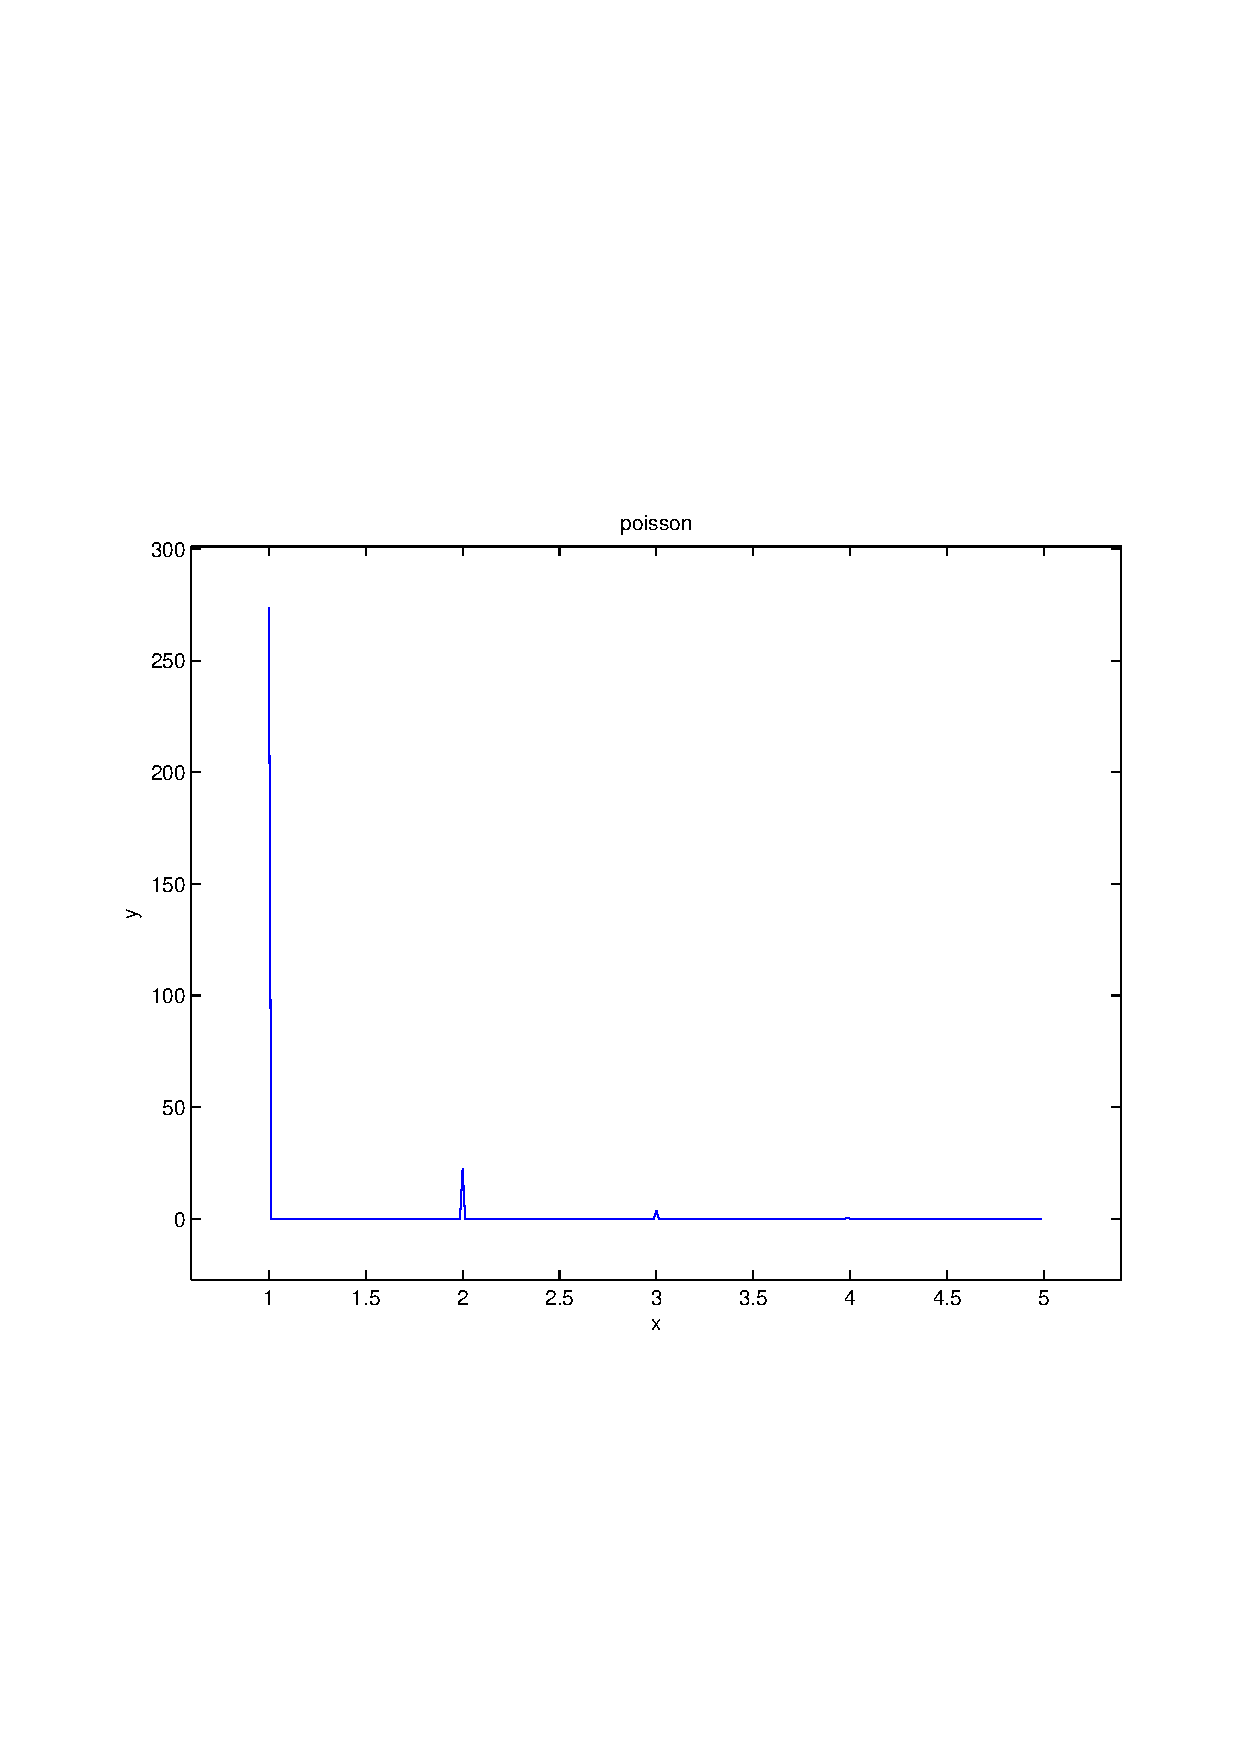
\includegraphics[width=5cm,height=5cm]{poisson.pdf}

\newpage
beta \begin{tabular}{|c|c|c|c|}  mean & variance & skewness & kurtosis \\  \hline
$\mu_1 = +0.33346$ & $\mu_2 = +0.12707$ & $\mu_3 = +0.68150$ & $\mu_4 =+1.91153$ \\
\end{tabular}

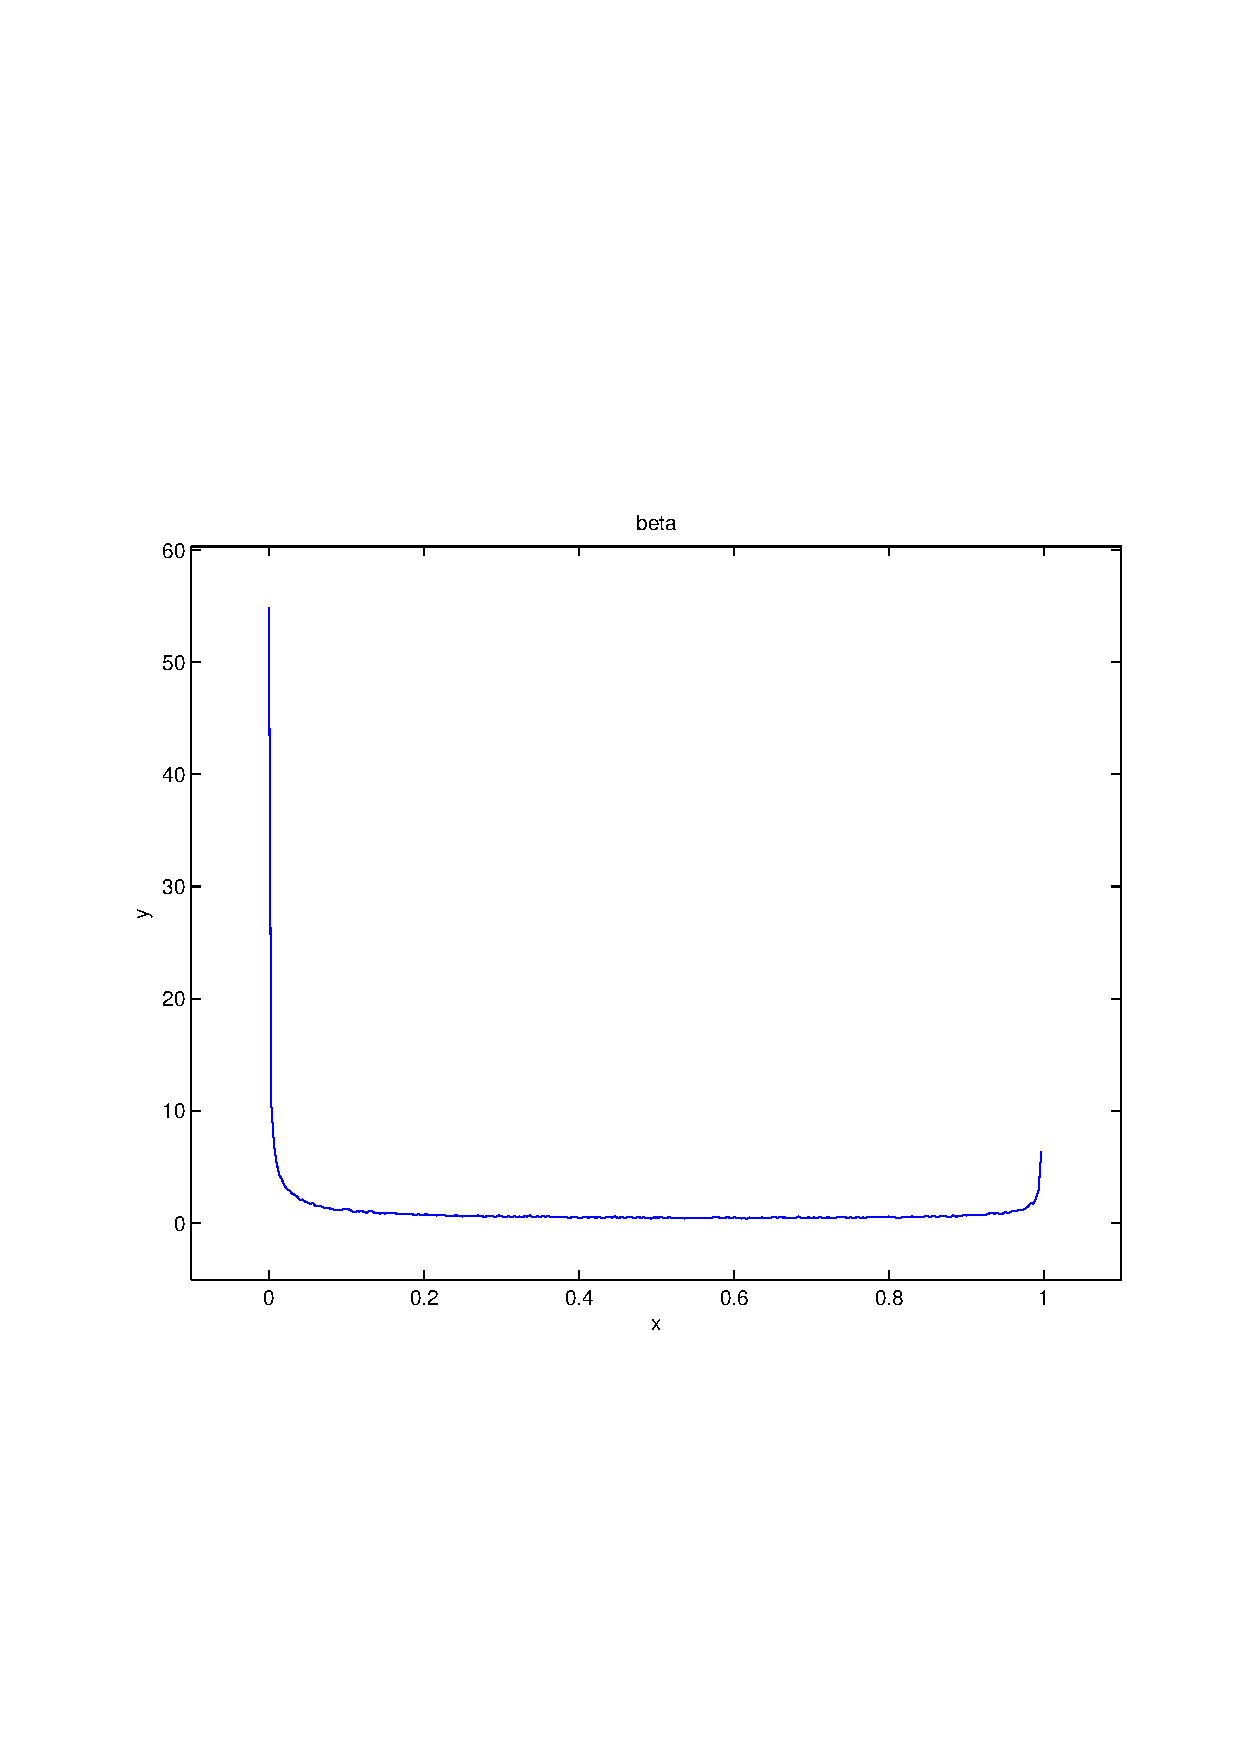
\includegraphics[width=5cm,height=5cm]{beta.pdf}

QueryPerformanceCounter  =  +20.51219
\subsubsection{Multiclass Support Vector Machine }
\begin{itemize}
\item Number or training points = 1024
\item Feature dimension = 3
\item Number or classes = 3
\end{itemize}
{The mean vectors of the 3 classes}

$\mu_1 = \left(
\begin{array}{
ccc}
+1.90000 & +0.10000 & +0.10000 \\
\end{array}
\right)$ \newline 

$\mu_2 = \left(
\begin{array}{
ccc}
+0.10000 & +1.90000 & +0.10000 \\
\end{array}
\right)$ \newline 

$\mu_3 = \left(
\begin{array}{
ccc}
+0.00000 & +0.00000 & +1.90000 \\
\end{array}
\right)$ \newline 

A random SPD covairance matrix is generated for each of the classes.\newline

$\rho_1 = \left(
\begin{array}{
ccc}
+3.165 & +0.114 & +0.366 \\
+0.114 & +3.906 & -0.346 \\
+0.366 & -0.346 & +3.775 \\
\end{array}
\right)$ \newline 

$\rho_2 = \left(
\begin{array}{
ccc}
+1.877 & +0.413 & +0.244 \\
+0.413 & +2.597 & +0.169 \\
+0.244 & +0.169 & +2.981 \\
\end{array}
\right)$ \newline 

$\rho_3 = \left(
\begin{array}{
ccc}
+4.086 & -0.432 & +0.413 \\
-0.432 & +2.370 & -0.480 \\
+0.413 & -0.480 & +3.272 \\
\end{array}
\right)$ \newline 

Verify $L_1$ condition number of covariance. The diagonal entries of the matrix have the form $(0.5 + U(0,1) )*dim(Dom(Cov))$
The lower-diagonal entries take the form $U(0,1) - 0.5$. 
The $L_1$ condition numbers are :
\begin{itemize}
\item +1.635
\item +2.320
\item +2.672
\end{itemize}
\includegraphics[width=10.0cm,height=10.0cm]{rv1_corr.pdf}

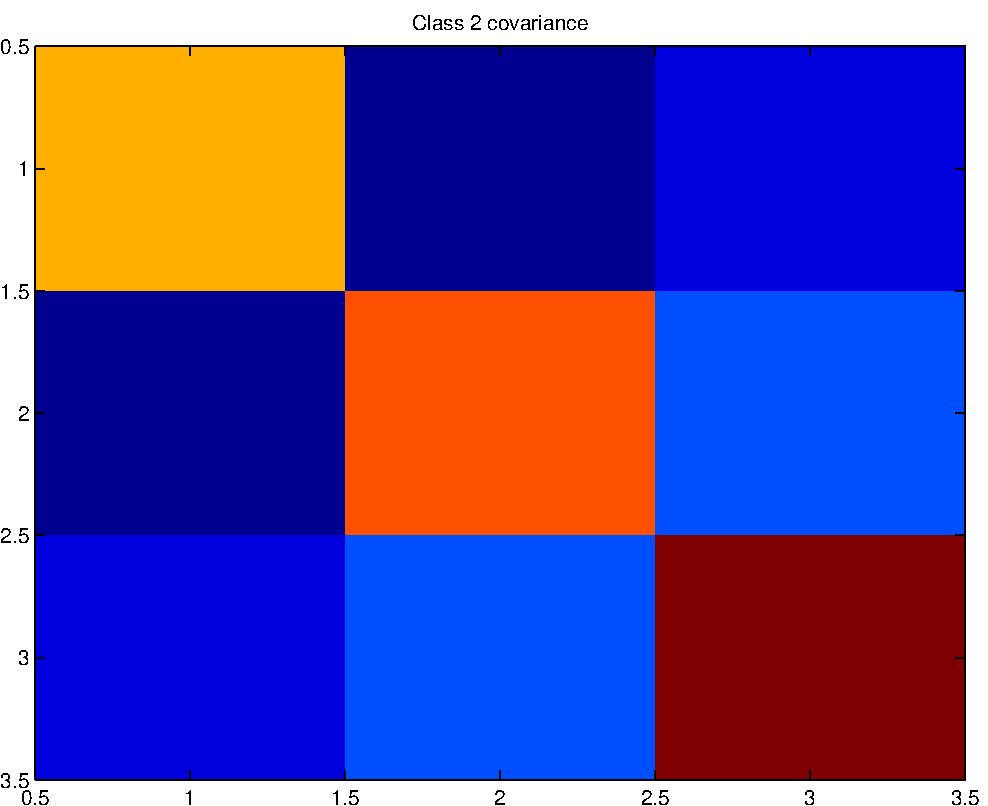
\includegraphics[width=10.0cm,height=10.0cm]{rv2_corr.pdf}

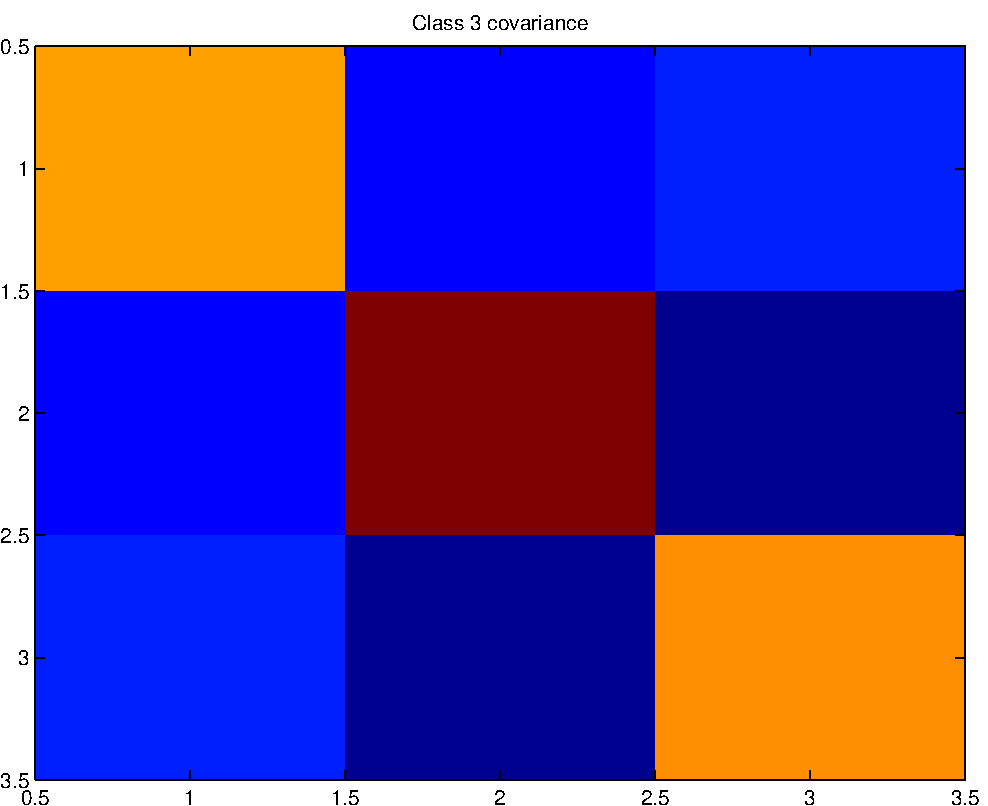
\includegraphics[width=10.0cm,height=10.0cm]{rv3_corr.pdf}

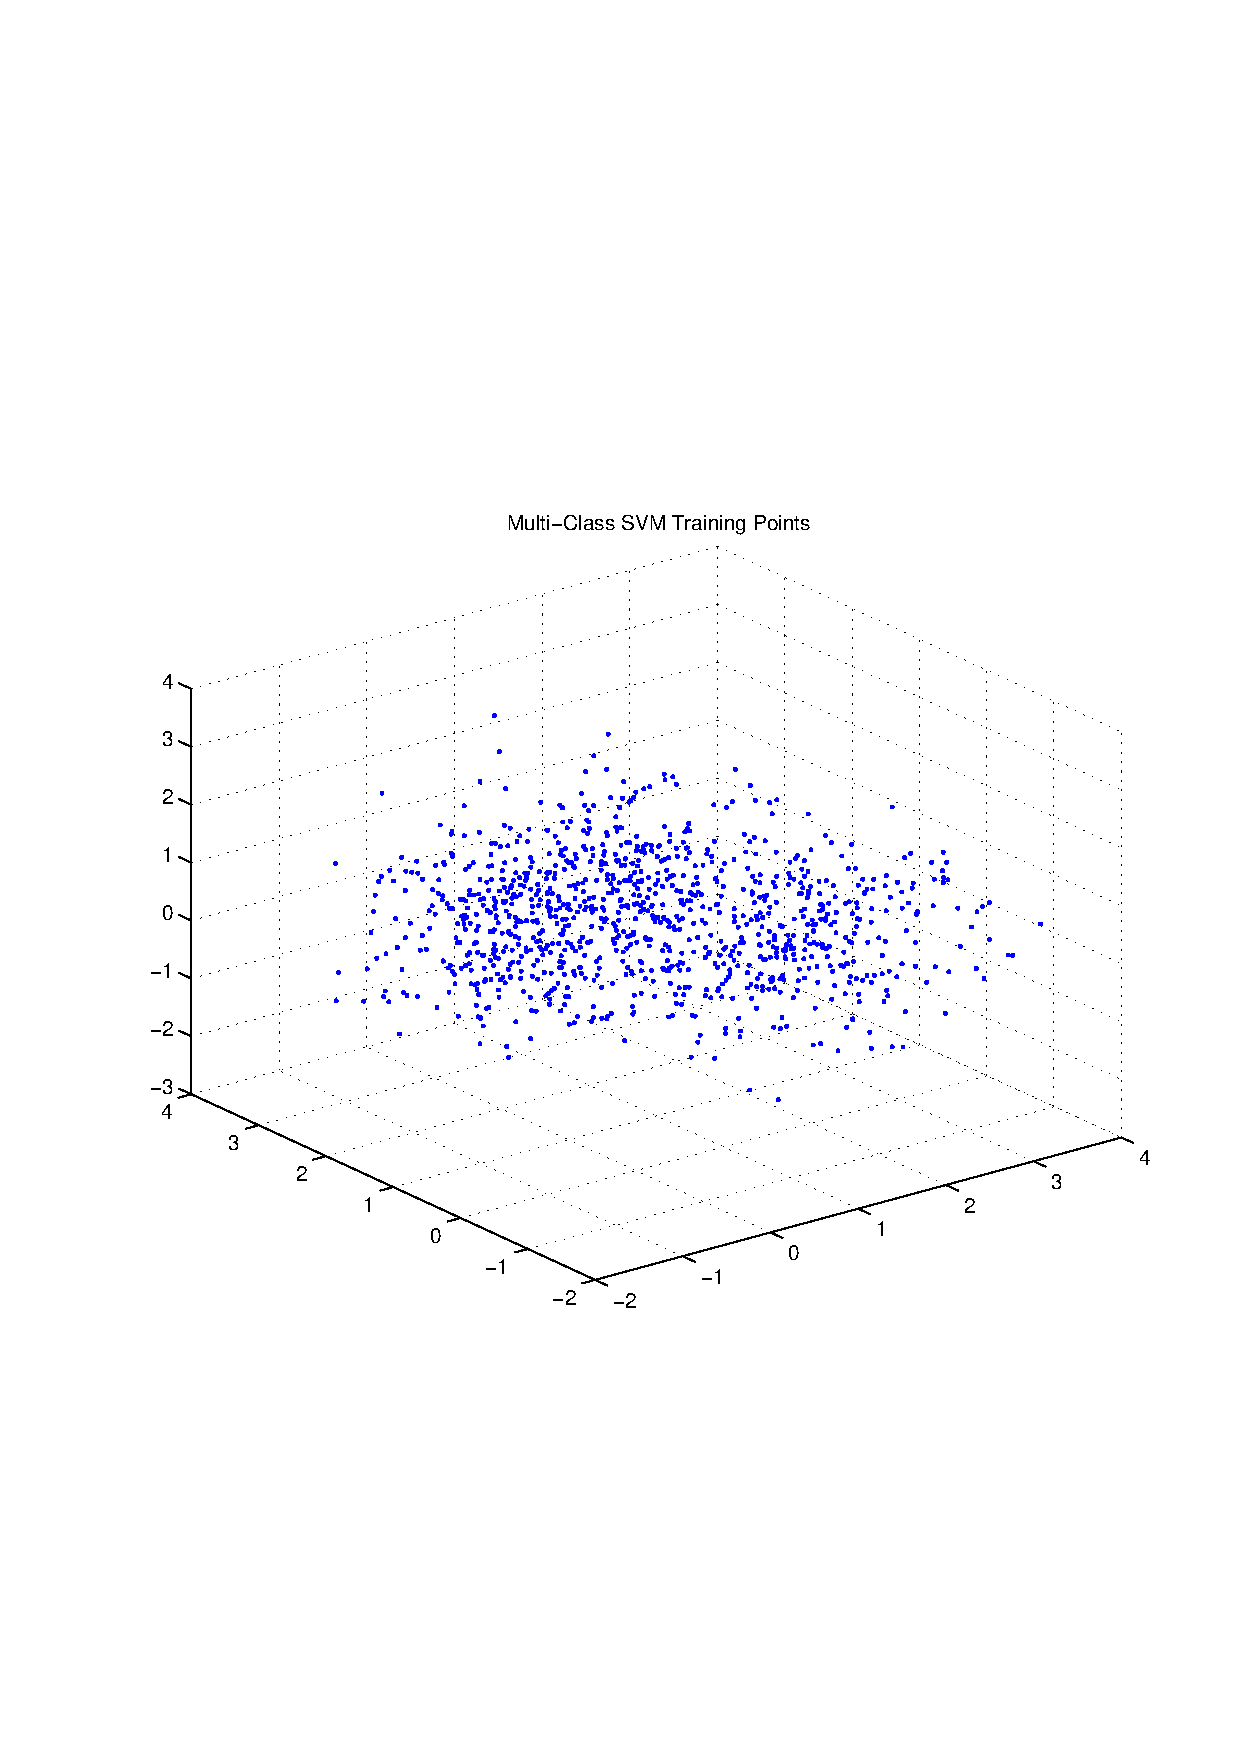
\includegraphics[width=10.0cm,height=10.0cm]{trainingPoints.pdf}

These are the SVM parameters - the RBF kernel is used\begin{itemize}
\item allOutlierFraction=0.05
\item mixingCoeff=0.3
\item smoThresh=1.0/10000.0
\item sigma=1
\end{itemize}
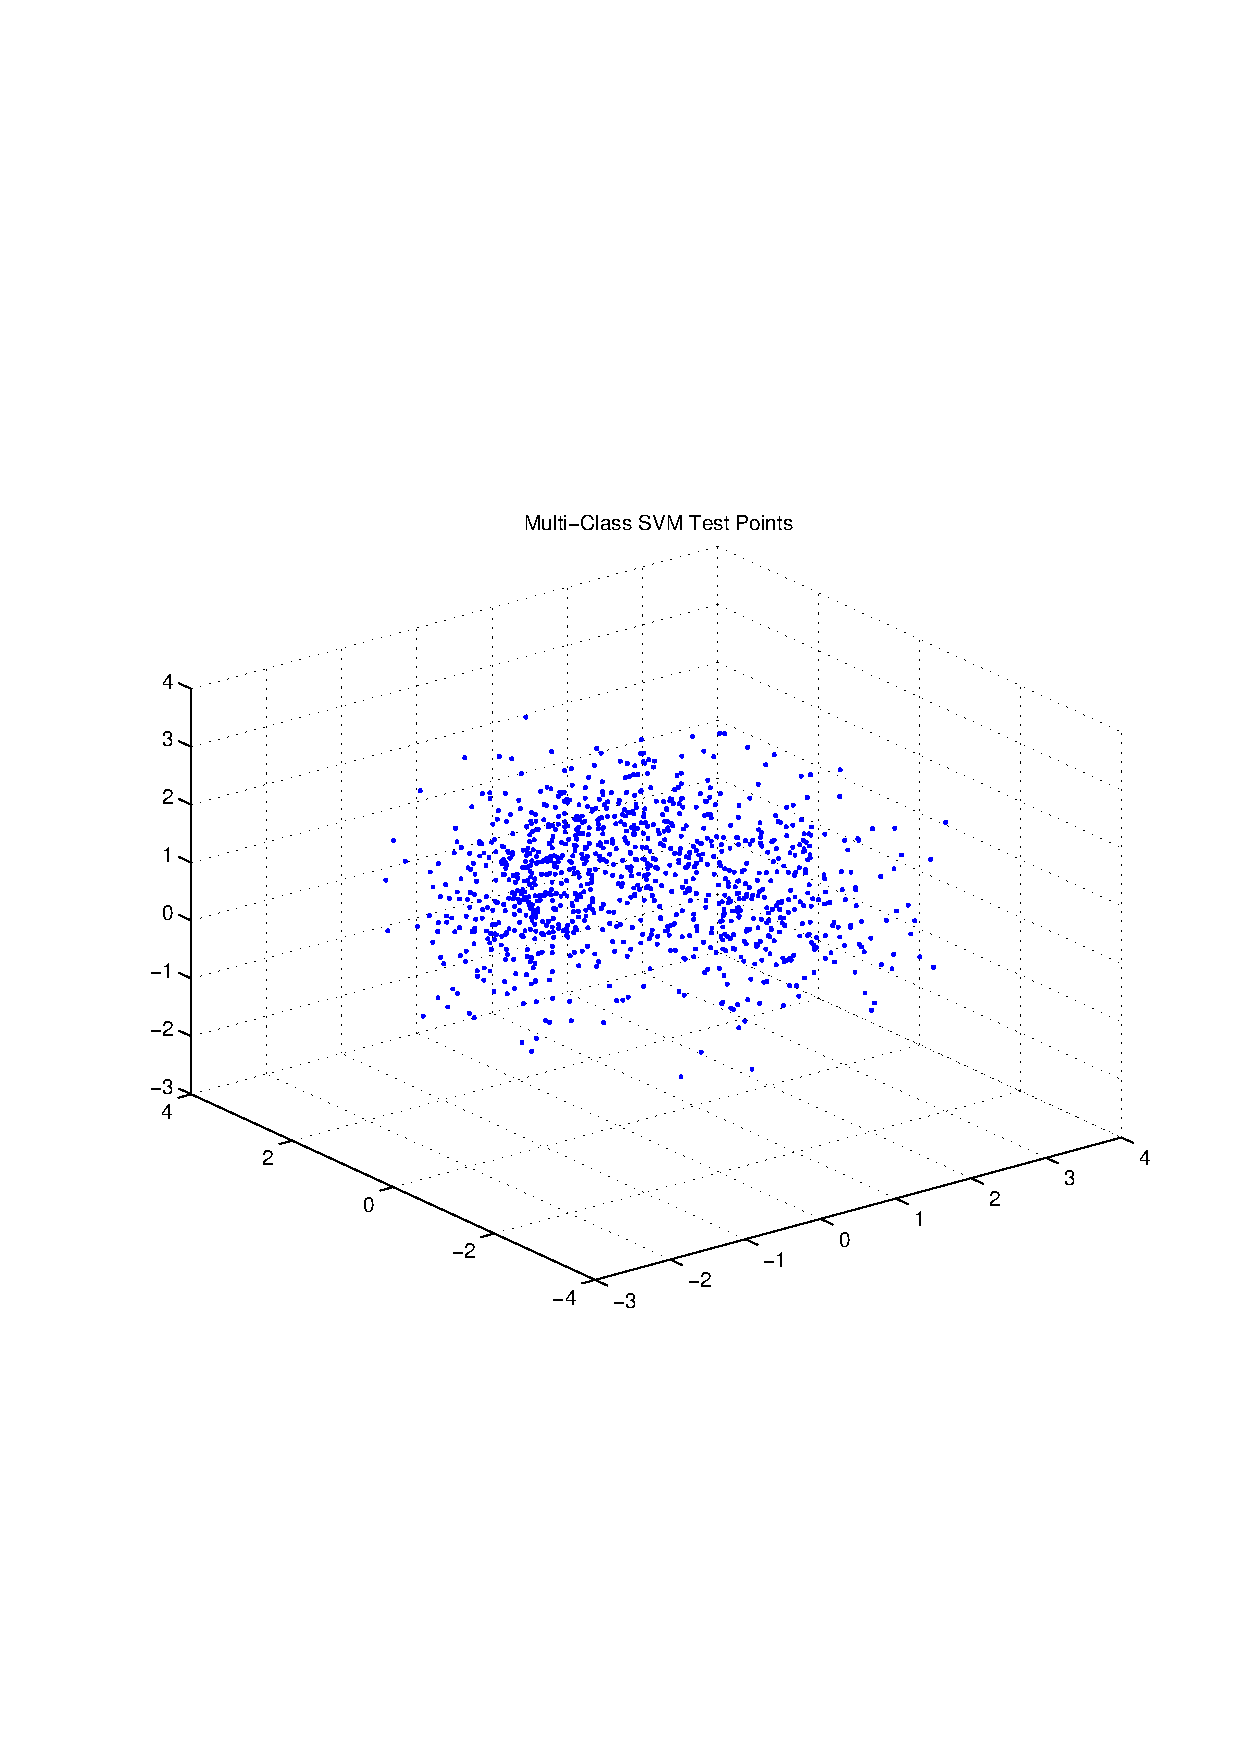
\includegraphics[width=10.0cm,height=10.0cm]{testPoints.pdf}

The marginal sample moments (mean var skew kurtosis) for training points.\newline
\begin{tabular}{ c |  c  c  c  c}
Feature & $\mu_1$ & $\mu_2$ & $\mu_3$ & $\mu_4$ \\
0 & +0.669 & +1.368 & +0.235& +2.438 \\
\hline
1 & +0.703 & +1.270 & +0.286& +2.333 \\
\hline
2 & +0.700 & +1.379 & +0.270& +2.519 \\
\hline
\end{tabular}
\newline
The marginal sample moments (mean var skew kurtosis) for test points.\newline
\begin{tabular}{ c | c  c  c  c}
Feature & $\mu_1$ & $\mu_2$ & $\mu_3$ & $\mu_4$ \\
0 & +0.677 & +1.280 & +0.359& +2.580\\
\hline
1 & +0.666 & +1.272 & +0.300& +2.319\\
\hline
2 & +0.725 & +1.294 & +0.276& +2.456\\
\hline
\end{tabular}\newline
\includegraphics[width=10.0cm,height=10.0cm]{classDiffs.pdf}

The error rate for this run is +0.167\newline
QueryPerformanceCounter  =  +6.884
\subsubsection{Semidefinite Programming SDPA}
QueryPerformanceCounter  =  +0.048
\subsubsection{Linear Regression 3x1}
\subsubsection{3 x 1 Linear Regression}
Sample size = 64

Number of features = 3

$\sigma = \left(
\begin{array}{
ccc}
+3.952 & -0.499 & -0.010 \\
-0.499 & +1.895 & +0.465 \\
-0.010 & +0.465 & +4.477 \\
\end{array}
\right)$ \newline 

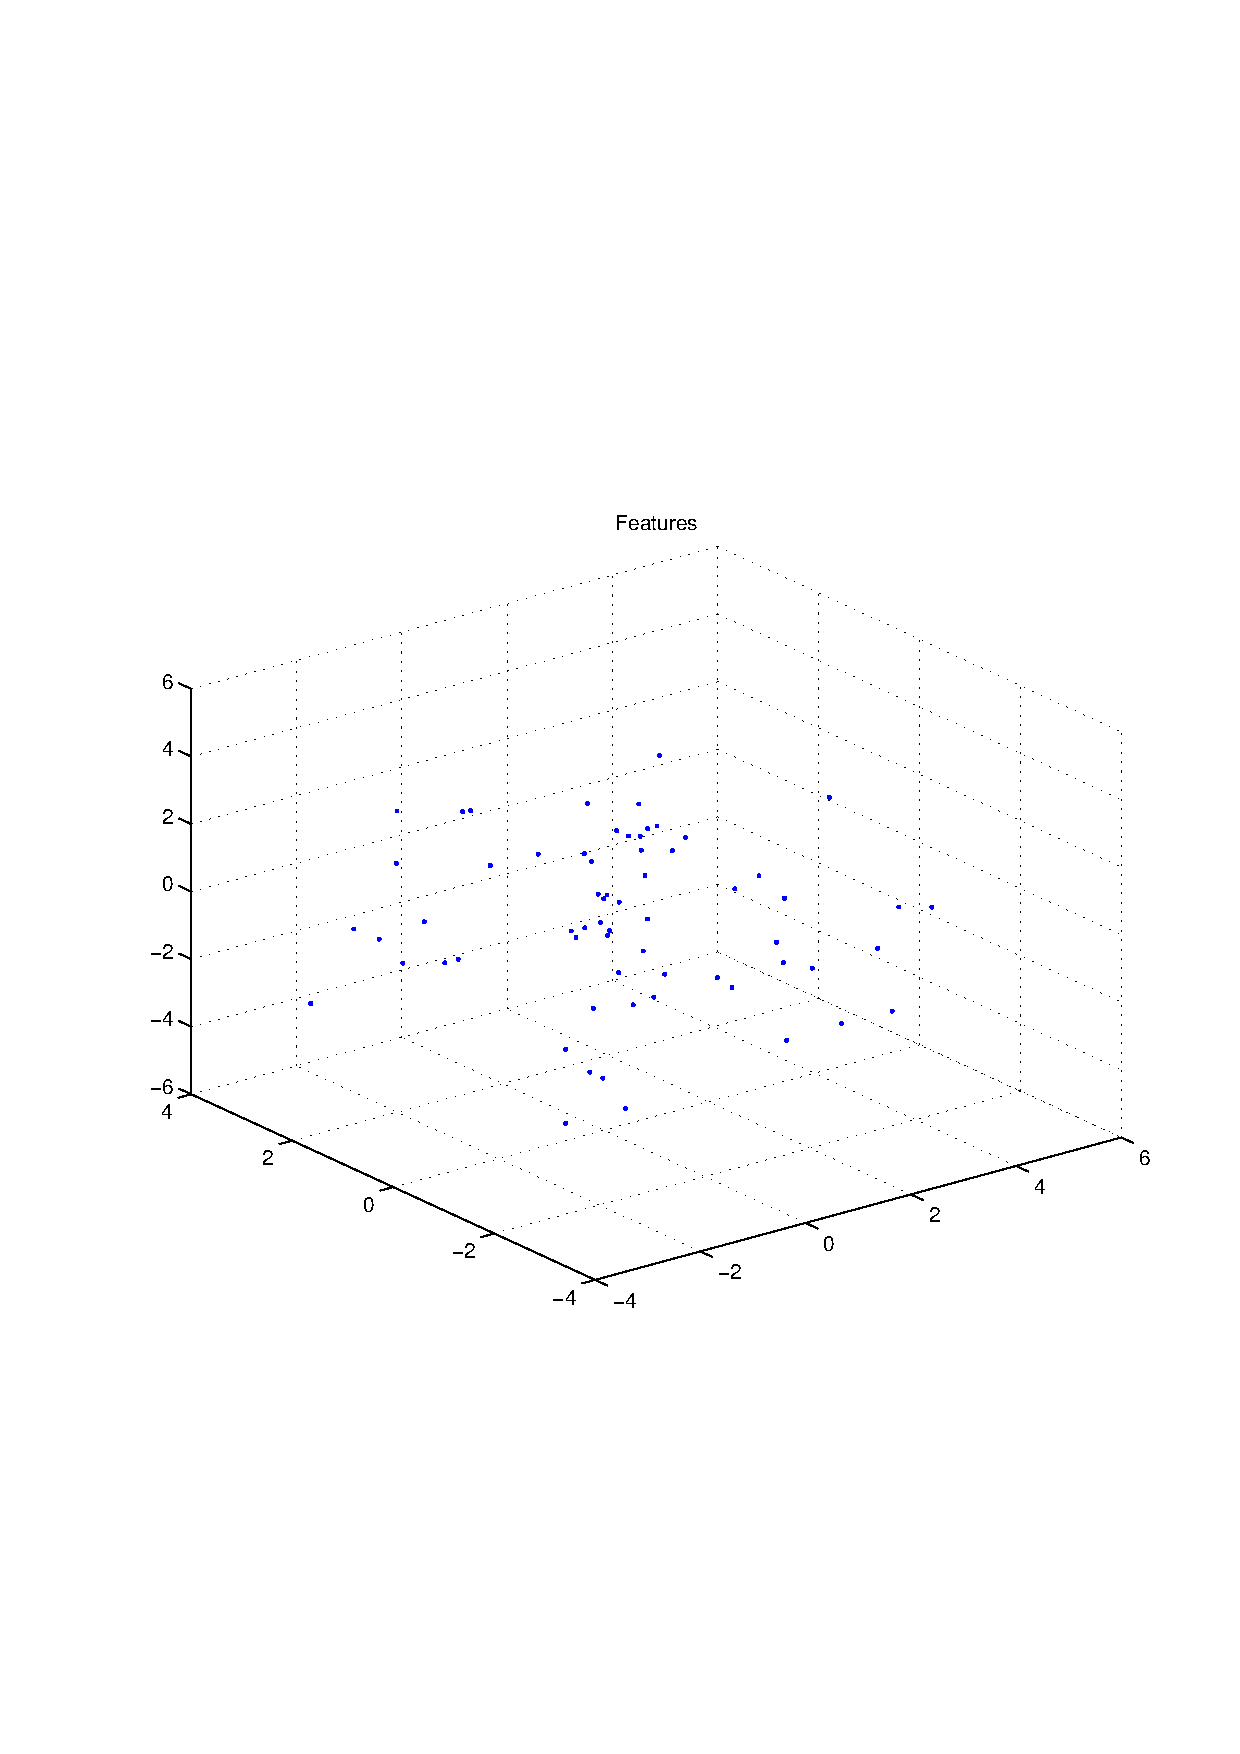
\includegraphics[width=10.0cm,height=10.0cm]{regression_features.pdf}

Beta
+0.817, +0.999, +0.510

Response
-3.974
+2.132
+0.098
+1.029
-2.609
+2.220
-1.376
+2.617
+4.250
+0.549
+1.307
+1.528
+1.775
+3.769
-0.605
+3.418
+2.074
+3.594
-0.834
+4.423
-0.048
+2.778
-2.507
+2.509
-0.203
+2.121
+2.736
-0.274
+2.031
+0.220
-0.108
+2.125
-2.906
-0.472
+5.784
+2.810
+1.903
+1.708
-1.644
+3.254
-1.788
+1.514
-2.928
-0.179
-0.278
+1.423
+0.045
-1.444
+0.370
+5.540
-3.691
-1.150
+0.748
-3.959
-2.969
-2.845
-3.185
-1.705
-0.886
+0.357
+4.216
+2.468
+2.668
+2.603
Estimate for Beta
-6277438562204192200000000000000000000000000000000000000000000000000.000
-6277438562204192200000000000000000000000000000000000000000000000000.000
-6277438562204192200000000000000000000000000000000000000000000000000.000
Error:
-0.000, -0.000, -0.000


QueryPerformanceCounter  =  +1.054
\subsubsection{Matrix Norms}
\subsubsection{Haar Distributed Random Orthogonal Matrix $A \in O(n)$}
 Testing Operator Norm
Number of Dimensions: +12

$A = \left(
\begin{array}{
cccccccccccc}
-0.209 & +0.035 & +0.628 & -0.121 & -0.193 & -0.264 & -0.037 & -0.161 & +0.044 & -0.169 & +0.061 & +0.615 \\
-0.036 & +0.043 & -0.299 & -0.294 & -0.313 & +0.319 & +0.021 & +0.623 & +0.040 & +0.045 & +0.221 & +0.424 \\
+0.206 & +0.101 & -0.359 & +0.379 & +0.025 & -0.146 & -0.019 & -0.186 & +0.163 & -0.536 & +0.518 & +0.191 \\
+0.402 & +0.476 & +0.027 & +0.398 & -0.012 & +0.232 & -0.312 & -0.005 & -0.092 & +0.152 & -0.406 & +0.325 \\
+0.239 & +0.032 & +0.442 & -0.102 & -0.098 & +0.573 & -0.232 & -0.142 & +0.201 & +0.022 & +0.451 & -0.281 \\
+0.178 & -0.440 & +0.058 & +0.113 & -0.337 & -0.260 & -0.602 & +0.249 & -0.326 & -0.152 & -0.013 & -0.157 \\
-0.459 & +0.068 & -0.050 & +0.045 & +0.001 & +0.468 & -0.023 & -0.164 & -0.583 & -0.432 & -0.086 & -0.012 \\
+0.624 & -0.298 & -0.023 & -0.271 & -0.112 & +0.089 & +0.432 & -0.264 & -0.363 & -0.062 & -0.072 & +0.175 \\
-0.003 & -0.436 & +0.116 & +0.273 & -0.044 & +0.294 & +0.181 & +0.167 & +0.487 & -0.378 & -0.437 & +0.030 \\
-0.174 & -0.501 & -0.258 & +0.076 & +0.210 & +0.209 & -0.302 & -0.380 & +0.073 & +0.404 & +0.088 & +0.383 \\
+0.064 & -0.170 & +0.321 & +0.363 & +0.555 & +0.026 & +0.204 & +0.439 & -0.301 & +0.107 & +0.275 & +0.111 \\
-0.167 & -0.041 & +0.036 & +0.535 & -0.612 & +0.020 & +0.363 & -0.086 & -0.097 & +0.358 & +0.155 & -0.081 \\
\end{array}
\right)$ \newline 

$Det(A) :   A \in O(n)$ = (+1.000,+0.000)

$L = \left(
\begin{array}{
cccccccccccc}
+1.000 & +0.000 & +0.000 & +0.000 & +0.000 & +0.000 & +0.000 & +0.000 & +0.000 & +0.000 & +0.000 & +0.000 \\
+0.644 & +1.000 & +0.000 & +0.000 & +0.000 & +0.000 & +0.000 & +0.000 & +0.000 & +0.000 & +0.000 & +0.000 \\
-0.335 & -0.097 & +1.000 & +0.000 & +0.000 & +0.000 & +0.000 & +0.000 & +0.000 & +0.000 & +0.000 & +0.000 \\
-0.005 & -0.656 & +0.230 & +1.000 & +0.000 & +0.000 & +0.000 & +0.000 & +0.000 & +0.000 & +0.000 & +0.000 \\
-0.268 & -0.181 & +0.060 & +0.842 & +1.000 & +0.000 & +0.000 & +0.000 & +0.000 & +0.000 & +0.000 & +0.000 \\
-0.057 & +0.039 & -0.485 & -0.597 & +0.612 & +1.000 & +0.000 & +0.000 & +0.000 & +0.000 & +0.000 & +0.000 \\
+0.284 & -0.533 & +0.139 & +0.757 & +0.421 & -0.573 & +1.000 & +0.000 & +0.000 & +0.000 & +0.000 & +0.000 \\
+0.103 & -0.209 & +0.532 & +0.868 & -1.000 & -0.789 & -0.341 & +1.000 & +0.000 & +0.000 & +0.000 & +0.000 \\
-0.735 & -0.225 & -0.092 & -0.058 & +0.130 & +0.924 & -0.321 & -0.855 & +1.000 & +0.000 & +0.000 & +0.000 \\
-0.279 & -0.876 & -0.365 & +0.651 & -0.180 & -0.068 & +0.350 & -0.943 & +0.568 & +1.000 & +0.000 & +0.000 \\
+0.329 & +0.298 & -0.583 & +0.302 & +0.154 & -0.668 & +0.168 & +0.145 & -0.357 & -0.852 & +1.000 & +0.000 \\
+0.383 & +0.219 & +0.709 & -0.020 & -0.140 & +0.931 & -0.086 & -0.755 & +0.489 & +0.784 & +0.680 & +1.000 \\
\end{array}
\right)$ \newline 

$U = \left(
\begin{array}{
cccccccccccc}
+0.624 & -0.298 & -0.023 & -0.271 & -0.112 & +0.089 & +0.432 & -0.264 & -0.363 & -0.062 & -0.072 & +0.175 \\
+0.000 & +0.667 & +0.042 & +0.572 & +0.061 & +0.174 & -0.590 & +0.165 & +0.142 & +0.192 & -0.360 & +0.212 \\
+0.000 & +0.000 & +0.624 & -0.156 & -0.224 & -0.217 & +0.051 & -0.233 & -0.064 & -0.171 & +0.002 & +0.694 \\
+0.000 & +0.000 & +0.000 & +0.683 & +0.047 & +0.459 & -0.216 & +0.328 & +0.593 & -0.213 & -0.674 & +0.010 \\
+0.000 & +0.000 & +0.000 & +0.000 & -0.658 & -0.298 & +0.551 & -0.389 & -0.664 & +0.566 & +0.639 & -0.045 \\
+0.000 & +0.000 & +0.000 & +0.000 & +0.000 & +0.668 & -0.373 & +0.922 & +0.744 & -0.523 & -0.562 & +0.795 \\
+0.000 & +0.000 & +0.000 & +0.000 & +0.000 & +0.000 & -1.329 & +0.889 & +0.119 & -0.384 & -0.266 & +0.277 \\
+0.000 & +0.000 & +0.000 & +0.000 & +0.000 & +0.000 & +0.000 & +0.982 & -0.751 & +0.451 & +0.895 & +0.437 \\
+0.000 & +0.000 & +0.000 & +0.000 & +0.000 & +0.000 & +0.000 & +0.000 & -1.995 & +0.210 & +0.857 & -0.037 \\
+0.000 & +0.000 & +0.000 & +0.000 & +0.000 & +0.000 & +0.000 & +0.000 & +0.000 & +1.138 & +0.720 & +1.246 \\
+0.000 & +0.000 & +0.000 & +0.000 & +0.000 & +0.000 & +0.000 & +0.000 & +0.000 & +0.000 & +1.213 & +1.948 \\
+0.000 & +0.000 & +0.000 & +0.000 & +0.000 & +0.000 & +0.000 & +0.000 & +0.000 & +0.000 & +0.000 & -3.562 \\
\end{array}
\right)$ \newline 

$L * U  = \left(
\begin{array}{
cccccccccccc}
+0.624 & -0.298 & -0.023 & -0.271 & -0.112 & +0.089 & +0.432 & -0.264 & -0.363 & -0.062 & -0.072 & +0.175 \\
+0.402 & +0.476 & +0.027 & +0.398 & -0.012 & +0.232 & -0.312 & -0.005 & -0.092 & +0.152 & -0.406 & +0.325 \\
-0.209 & +0.035 & +0.628 & -0.121 & -0.193 & -0.264 & -0.037 & -0.161 & +0.044 & -0.169 & +0.061 & +0.615 \\
-0.003 & -0.436 & +0.116 & +0.273 & -0.044 & +0.294 & +0.181 & +0.167 & +0.487 & -0.378 & -0.437 & +0.030 \\
-0.167 & -0.041 & +0.036 & +0.535 & -0.612 & +0.020 & +0.363 & -0.086 & -0.097 & +0.358 & +0.155 & -0.081 \\
-0.036 & +0.043 & -0.299 & -0.294 & -0.313 & +0.319 & +0.021 & +0.623 & +0.040 & +0.045 & +0.221 & +0.424 \\
+0.178 & -0.440 & +0.058 & +0.113 & -0.337 & -0.260 & -0.602 & +0.249 & -0.326 & -0.152 & -0.013 & -0.157 \\
+0.064 & -0.170 & +0.321 & +0.363 & +0.555 & +0.026 & +0.204 & +0.439 & -0.301 & +0.107 & +0.275 & +0.111 \\
-0.459 & +0.068 & -0.050 & +0.045 & +0.001 & +0.468 & -0.023 & -0.164 & -0.583 & -0.432 & -0.086 & -0.012 \\
-0.174 & -0.501 & -0.258 & +0.076 & +0.210 & +0.209 & -0.302 & -0.380 & +0.073 & +0.404 & +0.088 & +0.383 \\
+0.206 & +0.101 & -0.359 & +0.379 & +0.025 & -0.146 & -0.019 & -0.186 & +0.163 & -0.536 & +0.518 & +0.191 \\
+0.239 & +0.032 & +0.442 & -0.102 & -0.098 & +0.573 & -0.232 & -0.142 & +0.201 & +0.022 & +0.451 & -0.281 \\
\end{array}
\right)$ \newline 

$Det(L) :    = (+1.000,+0.000)     Det(U) :    = (+1.000,+0.000)     Det(LU) :    = (+1.000,+0.000)$

$||A||_{L_1}$  = +2.970

$||A||_{L_{\infty}}$ = +3.058

$||A^{-1}||_{L_1}$  = +3.058

$||A^{-1}||_{L_{\infty}}$ = +2.970

$||A||_{L_{\infty}} * ||A^{-1}||_{L_{\infty}} = +9.081$

$||A||_{L_1} * ||A^{-1}||_{L_1} = +9.081$

Frobenious Norm  $||A||_{\textit{F}}$ via $\sum\limits_{i,j =0}^{n} \|A_{i,j}|$   of  $A \in O(n)$  +3.464

$L_1$ condition number of Haar Distributed Random Orthogonal Matrix $A \in O(n)$ +8.562

$A = \left(
\begin{array}{
cccccccccccc}
-0.209 & +0.035 & +0.628 & -0.121 & -0.193 & -0.264 & -0.037 & -0.161 & +0.044 & -0.169 & +0.061 & +0.615 \\
-0.036 & +0.043 & -0.299 & -0.294 & -0.313 & +0.319 & +0.021 & +0.623 & +0.040 & +0.045 & +0.221 & +0.424 \\
+0.206 & +0.101 & -0.359 & +0.379 & +0.025 & -0.146 & -0.019 & -0.186 & +0.163 & -0.536 & +0.518 & +0.191 \\
+0.402 & +0.476 & +0.027 & +0.398 & -0.012 & +0.232 & -0.312 & -0.005 & -0.092 & +0.152 & -0.406 & +0.325 \\
+0.239 & +0.032 & +0.442 & -0.102 & -0.098 & +0.573 & -0.232 & -0.142 & +0.201 & +0.022 & +0.451 & -0.281 \\
+0.178 & -0.440 & +0.058 & +0.113 & -0.337 & -0.260 & -0.602 & +0.249 & -0.326 & -0.152 & -0.013 & -0.157 \\
-0.459 & +0.068 & -0.050 & +0.045 & +0.001 & +0.468 & -0.023 & -0.164 & -0.583 & -0.432 & -0.086 & -0.012 \\
+0.624 & -0.298 & -0.023 & -0.271 & -0.112 & +0.089 & +0.432 & -0.264 & -0.363 & -0.062 & -0.072 & +0.175 \\
-0.003 & -0.436 & +0.116 & +0.273 & -0.044 & +0.294 & +0.181 & +0.167 & +0.487 & -0.378 & -0.437 & +0.030 \\
-0.174 & -0.501 & -0.258 & +0.076 & +0.210 & +0.209 & -0.302 & -0.380 & +0.073 & +0.404 & +0.088 & +0.383 \\
+0.064 & -0.170 & +0.321 & +0.363 & +0.555 & +0.026 & +0.204 & +0.439 & -0.301 & +0.107 & +0.275 & +0.111 \\
-0.167 & -0.041 & +0.036 & +0.535 & -0.612 & +0.020 & +0.363 & -0.086 & -0.097 & +0.358 & +0.155 & -0.081 \\
\end{array}
\right)$ \newline 

$L_{\infty}$ condition number of Haar Distributed Random Orthogonal Matrix $A \in O(n)$ +8.472

Eigenvalues of $A \in O(n)$

(-1.000,+0.024), (-1.000,-0.024), (-0.595,+0.803), (-0.595,-0.803), (-0.111,+0.994), (-0.111,-0.994), (+0.047,+0.999), (+0.047,-0.999), (+0.838,+0.546), (+0.838,-0.546), (+0.978,+0.206), (+0.978,-0.206)

 $|\lambda | : \lambda \in \sigma(A) , A \in O(n)$

+1.000, +1.000, +1.000, +1.000, +1.000, +1.000, +1.000, +1.000, +1.000, +1.000, +1.000, +1.000


Calculating $A^{\dag} A,$  we expect $A^{\dag} A \approx I$

$A^{\dag} A = \left(
\begin{array}{
cccccccccccc}
+1.000 & -0.000 & +0.000 & +0.000 & -0.000 & +0.000 & -0.000 & -0.000 & +0.000 & -0.000 & +0.000 & +0.000 \\
-0.000 & +1.000 & +0.000 & +0.000 & +0.000 & -0.000 & -0.000 & -0.000 & -0.000 & +0.000 & -0.000 & +0.000 \\
+0.000 & +0.000 & +1.000 & -0.000 & -0.000 & +0.000 & -0.000 & -0.000 & +0.000 & +0.000 & -0.000 & -0.000 \\
+0.000 & +0.000 & -0.000 & +1.000 & -0.000 & -0.000 & -0.000 & -0.000 & -0.000 & -0.000 & -0.000 & +0.000 \\
-0.000 & +0.000 & -0.000 & -0.000 & +1.000 & -0.000 & +0.000 & +0.000 & -0.000 & +0.000 & -0.000 & +0.000 \\
+0.000 & -0.000 & +0.000 & -0.000 & -0.000 & +1.000 & -0.000 & -0.000 & +0.000 & +0.000 & +0.000 & -0.000 \\
-0.000 & -0.000 & -0.000 & -0.000 & +0.000 & -0.000 & +1.000 & -0.000 & +0.000 & -0.000 & -0.000 & +0.000 \\
-0.000 & -0.000 & -0.000 & -0.000 & +0.000 & -0.000 & -0.000 & +1.000 & -0.000 & +0.000 & -0.000 & +0.000 \\
+0.000 & -0.000 & +0.000 & -0.000 & -0.000 & +0.000 & +0.000 & -0.000 & +1.000 & -0.000 & +0.000 & -0.000 \\
-0.000 & +0.000 & +0.000 & -0.000 & +0.000 & +0.000 & -0.000 & +0.000 & -0.000 & +1.000 & -0.000 & +0.000 \\
+0.000 & -0.000 & -0.000 & -0.000 & -0.000 & +0.000 & -0.000 & -0.000 & +0.000 & -0.000 & +1.000 & -0.000 \\
+0.000 & +0.000 & -0.000 & +0.000 & +0.000 & -0.000 & +0.000 & +0.000 & -0.000 & +0.000 & -0.000 & +1.000 \\
\end{array}
\right)$ \newline 

Calculating $A^{-1} ,  A \in O(n)$.

$A^{-1} = \left(
\begin{array}{
cccccccccccc}
-0.209 & -0.036 & +0.206 & +0.402 & +0.239 & +0.178 & -0.459 & +0.624 & -0.003 & -0.174 & +0.064 & -0.167 \\
+0.035 & +0.043 & +0.101 & +0.476 & +0.032 & -0.440 & +0.068 & -0.298 & -0.436 & -0.501 & -0.170 & -0.041 \\
+0.628 & -0.299 & -0.359 & +0.027 & +0.442 & +0.058 & -0.050 & -0.023 & +0.116 & -0.258 & +0.321 & +0.036 \\
-0.121 & -0.294 & +0.379 & +0.398 & -0.102 & +0.113 & +0.045 & -0.271 & +0.273 & +0.076 & +0.363 & +0.535 \\
-0.193 & -0.313 & +0.025 & -0.012 & -0.098 & -0.337 & +0.001 & -0.112 & -0.044 & +0.210 & +0.555 & -0.612 \\
-0.264 & +0.319 & -0.146 & +0.232 & +0.573 & -0.260 & +0.468 & +0.089 & +0.294 & +0.209 & +0.026 & +0.020 \\
-0.037 & +0.021 & -0.019 & -0.312 & -0.232 & -0.602 & -0.023 & +0.432 & +0.181 & -0.302 & +0.204 & +0.363 \\
-0.161 & +0.623 & -0.186 & -0.005 & -0.142 & +0.249 & -0.164 & -0.264 & +0.167 & -0.380 & +0.439 & -0.086 \\
+0.044 & +0.040 & +0.163 & -0.092 & +0.201 & -0.326 & -0.583 & -0.363 & +0.487 & +0.073 & -0.301 & -0.097 \\
-0.169 & +0.045 & -0.536 & +0.152 & +0.022 & -0.152 & -0.432 & -0.062 & -0.378 & +0.404 & +0.107 & +0.358 \\
+0.061 & +0.221 & +0.518 & -0.406 & +0.451 & -0.013 & -0.086 & -0.072 & -0.437 & +0.088 & +0.275 & +0.155 \\
+0.615 & +0.424 & +0.191 & +0.325 & -0.281 & -0.157 & -0.012 & +0.175 & +0.030 & +0.383 & +0.111 & -0.081 \\
\end{array}
\right)$ \newline 

Calculating $A^{-1} *A  ,  A \in O(n)$.   We expect $A^{-1} *A  \approx I$. 

$A^{-1} *A = \left(
\begin{array}{
cccccccccccc}
+1.000 & +0.000 & +0.000 & +0.000 & +0.000 & +0.000 & -0.000 & +0.000 & +0.000 & +0.000 & +0.000 & -0.000 \\
-0.000 & +1.000 & +0.000 & -0.000 & +0.000 & +0.000 & -0.000 & -0.000 & +0.000 & +0.000 & +0.000 & +0.000 \\
+0.000 & +0.000 & +1.000 & -0.000 & +0.000 & +0.000 & +0.000 & -0.000 & +0.000 & -0.000 & +0.000 & +0.000 \\
+0.000 & -0.000 & +0.000 & +1.000 & -0.000 & -0.000 & +0.000 & -0.000 & +0.000 & +0.000 & +0.000 & +0.000 \\
-0.000 & -0.000 & +0.000 & -0.000 & +1.000 & -0.000 & +0.000 & -0.000 & -0.000 & -0.000 & -0.000 & -0.000 \\
+0.000 & -0.000 & +0.000 & -0.000 & -0.000 & +1.000 & -0.000 & +0.000 & -0.000 & -0.000 & +0.000 & +0.000 \\
+0.000 & -0.000 & +0.000 & -0.000 & +0.000 & +0.000 & +1.000 & +0.000 & +0.000 & +0.000 & -0.000 & +0.000 \\
-0.000 & +0.000 & +0.000 & +0.000 & +0.000 & +0.000 & -0.000 & +1.000 & +0.000 & -0.000 & -0.000 & +0.000 \\
-0.000 & -0.000 & -0.000 & -0.000 & -0.000 & -0.000 & +0.000 & -0.000 & +1.000 & +0.000 & +0.000 & -0.000 \\
-0.000 & +0.000 & +0.000 & -0.000 & -0.000 & -0.000 & +0.000 & +0.000 & +0.000 & +1.000 & -0.000 & +0.000 \\
+0.000 & -0.000 & +0.000 & -0.000 & +0.000 & +0.000 & -0.000 & +0.000 & +0.000 & +0.000 & +1.000 & -0.000 \\
-0.000 & +0.000 & -0.000 & +0.000 & -0.000 & -0.000 & -0.000 & +0.000 & -0.000 & +0.000 & -0.000 & +1.000 \\
\end{array}
\right)$ \newline 

Calculating SVD of  $A \in O(n)$

$U = \left(
\begin{array}{
cccccccccccc}
-0.040 & +0.374 & -0.130 & +0.186 & -0.333 & -0.275 & -0.196 & +0.078 & -0.255 & -0.232 & +0.649 & -0.189 \\
-0.049 & -0.081 & +0.267 & -0.057 & +0.593 & -0.030 & -0.606 & -0.304 & -0.171 & +0.049 & +0.143 & -0.227 \\
-0.062 & -0.058 & -0.343 & -0.543 & +0.279 & +0.315 & +0.009 & +0.192 & -0.079 & -0.291 & +0.350 & +0.390 \\
-0.162 & +0.355 & +0.043 & -0.260 & +0.308 & -0.461 & +0.236 & +0.324 & -0.382 & -0.108 & -0.365 & -0.139 \\
-0.061 & +0.320 & +0.033 & +0.126 & -0.039 & +0.181 & -0.536 & +0.609 & +0.171 & +0.279 & -0.163 & +0.225 \\
-0.125 & -0.416 & -0.380 & -0.282 & -0.384 & -0.351 & -0.392 & -0.085 & -0.253 & +0.182 & -0.226 & +0.088 \\
+0.043 & -0.167 & +0.062 & +0.252 & +0.142 & +0.031 & +0.261 & +0.112 & -0.540 & +0.593 & +0.274 & +0.287 \\
-0.380 & +0.333 & -0.475 & +0.357 & +0.241 & -0.101 & +0.007 & -0.419 & +0.117 & +0.038 & -0.120 & +0.344 \\
+0.133 & +0.066 & +0.043 & +0.244 & -0.158 & +0.447 & -0.137 & -0.118 & -0.584 & -0.421 & -0.359 & +0.110 \\
-0.209 & +0.035 & +0.628 & -0.121 & -0.193 & -0.264 & -0.037 & -0.161 & +0.044 & -0.169 & +0.061 & +0.615 \\
-0.830 & -0.050 & +0.140 & -0.091 & -0.175 & +0.362 & +0.098 & +0.019 & -0.079 & +0.101 & +0.041 & -0.300 \\
-0.223 & -0.550 & -0.031 & +0.481 & +0.211 & -0.209 & -0.011 & +0.392 & +0.078 & -0.407 & +0.025 & +0.040 \\
\end{array}
\right)$ \newline 

$S = \left(
\begin{array}{
cccccccccccc}
+1.000 & +0.000 & +0.000 & +0.000 & +0.000 & +0.000 & +0.000 & +0.000 & +0.000 & +0.000 & +0.000 & +0.000 \\
+0.000 & +1.000 & +0.000 & +0.000 & +0.000 & +0.000 & +0.000 & +0.000 & +0.000 & +0.000 & +0.000 & +0.000 \\
+0.000 & +0.000 & +1.000 & +0.000 & +0.000 & +0.000 & +0.000 & +0.000 & +0.000 & +0.000 & +0.000 & +0.000 \\
+0.000 & +0.000 & +0.000 & +1.000 & +0.000 & +0.000 & +0.000 & +0.000 & +0.000 & +0.000 & +0.000 & +0.000 \\
+0.000 & +0.000 & +0.000 & +0.000 & +1.000 & +0.000 & +0.000 & +0.000 & +0.000 & +0.000 & +0.000 & +0.000 \\
+0.000 & +0.000 & +0.000 & +0.000 & +0.000 & +1.000 & +0.000 & +0.000 & +0.000 & +0.000 & +0.000 & +0.000 \\
+0.000 & +0.000 & +0.000 & +0.000 & +0.000 & +0.000 & +1.000 & +0.000 & +0.000 & +0.000 & +0.000 & +0.000 \\
+0.000 & +0.000 & +0.000 & +0.000 & +0.000 & +0.000 & +0.000 & +1.000 & +0.000 & +0.000 & +0.000 & +0.000 \\
+0.000 & +0.000 & +0.000 & +0.000 & +0.000 & +0.000 & +0.000 & +0.000 & +1.000 & +0.000 & +0.000 & +0.000 \\
+0.000 & +0.000 & +0.000 & +0.000 & +0.000 & +0.000 & +0.000 & +0.000 & +0.000 & +1.000 & +0.000 & +0.000 \\
+0.000 & +0.000 & +0.000 & +0.000 & +0.000 & +0.000 & +0.000 & +0.000 & +0.000 & +0.000 & +1.000 & +0.000 \\
+0.000 & +0.000 & +0.000 & +0.000 & +0.000 & +0.000 & +0.000 & +0.000 & +0.000 & +0.000 & +0.000 & +1.000 \\
\end{array}
\right)$ \newline 

$V = \left(
\begin{array}{
cccccccccccc}
+0.000 & +0.000 & -0.000 & +0.000 & +0.000 & -0.000 & +0.000 & -0.000 & -0.000 & +1.000 & -0.000 & +0.000 \\
+0.105 & -0.532 & +0.622 & -0.112 & +0.486 & +0.116 & +0.126 & -0.178 & -0.046 & +0.000 & +0.080 & -0.030 \\
+0.551 & -0.072 & +0.223 & -0.321 & -0.238 & -0.212 & -0.171 & +0.362 & +0.032 & +0.000 & -0.426 & +0.307 \\
-0.104 & -0.006 & -0.264 & -0.062 & +0.551 & -0.154 & +0.085 & +0.265 & +0.503 & +0.000 & -0.426 & -0.276 \\
+0.124 & +0.314 & +0.037 & -0.582 & +0.047 & -0.416 & -0.118 & -0.477 & +0.029 & +0.000 & +0.160 & -0.321 \\
+0.302 & +0.214 & -0.196 & -0.090 & +0.173 & +0.586 & -0.035 & -0.460 & +0.257 & +0.000 & -0.160 & +0.372 \\
+0.117 & +0.120 & +0.271 & +0.113 & -0.158 & -0.019 & -0.001 & +0.180 & +0.736 & +0.000 & +0.533 & +0.054 \\
-0.249 & -0.239 & +0.173 & -0.049 & -0.568 & +0.108 & +0.267 & -0.319 & +0.309 & +0.000 & -0.426 & -0.253 \\
-0.542 & -0.315 & -0.119 & -0.263 & +0.014 & -0.202 & -0.381 & -0.105 & +0.171 & +0.000 & +0.047 & +0.543 \\
-0.358 & +0.326 & +0.192 & -0.564 & +0.009 & +0.373 & +0.328 & +0.381 & -0.105 & +0.000 & +0.053 & +0.072 \\
-0.029 & +0.218 & +0.080 & +0.186 & +0.098 & -0.457 & +0.657 & -0.182 & -0.011 & +0.000 & -0.080 & +0.469 \\
+0.264 & -0.493 & -0.542 & -0.312 & -0.114 & +0.014 & +0.420 & +0.069 & +0.014 & +0.000 & +0.320 & -0.008 \\
\end{array}
\right)$ \newline 

$U S V = \left(
\begin{array}{
cccccccccccc}
-0.066 & -0.157 & +0.296 & +0.558 & +0.318 & -0.302 & +0.523 & -0.032 & -0.157 & -0.040 & -0.277 & +0.023 \\
+0.225 & +0.417 & +0.000 & -0.355 & +0.195 & -0.359 & -0.130 & -0.190 & -0.586 & -0.049 & -0.279 & -0.077 \\
+0.185 & -0.017 & -0.214 & +0.079 & -0.302 & -0.009 & +0.341 & -0.735 & -0.108 & -0.062 & +0.367 & +0.123 \\
+0.154 & -0.167 & +0.592 & -0.028 & -0.293 & -0.094 & -0.108 & -0.056 & -0.033 & -0.162 & +0.192 & -0.651 \\
-0.253 & -0.466 & -0.006 & -0.442 & -0.051 & +0.356 & +0.221 & -0.234 & -0.106 & -0.061 & -0.515 & -0.102 \\
-0.300 & +0.074 & -0.336 & +0.295 & -0.270 & +0.252 & +0.068 & +0.305 & -0.609 & -0.125 & +0.115 & -0.264 \\
+0.169 & +0.420 & -0.023 & -0.310 & -0.058 & +0.104 & +0.703 & +0.301 & +0.221 & +0.043 & +0.038 & -0.217 \\
-0.141 & -0.210 & -0.238 & -0.198 & +0.654 & -0.070 & +0.050 & -0.022 & +0.028 & -0.380 & +0.441 & -0.256 \\
+0.641 & -0.067 & -0.264 & +0.296 & +0.255 & +0.405 & -0.112 & -0.075 & +0.044 & +0.133 & -0.223 & -0.334 \\
+0.492 & -0.505 & -0.165 & -0.155 & -0.222 & -0.293 & +0.102 & +0.410 & -0.159 & -0.209 & +0.032 & +0.262 \\
+0.102 & +0.262 & +0.170 & +0.110 & -0.042 & +0.295 & -0.061 & -0.018 & +0.098 & -0.830 & -0.164 & +0.247 \\
-0.147 & +0.047 & -0.469 & +0.119 & -0.247 & -0.478 & -0.067 & -0.083 & +0.388 & -0.223 & -0.349 & -0.347 \\
\end{array}
\right)$ \newline 

\subsubsection{Wishart Matrix $A \in W(n)$}
$L_1$ condition number of Wishart Matrix +56267.800
$L_infty$ condition number of Wishart Matrix +56267.800
\subsubsection{Gaussian Orthogonal Ensemble $A \in GOE(n)$}
$L_1$ condition number of GOE Matrix +470.231
$L_\infty$ condition number of GOE Matrix +470.231
\subsubsection{The Identity Matrix $I \in M(n)$}
$L_1$ condition number of $I$ = +1.000
$L_\infty$ condition number of $I$ = +1.000
QueryPerformanceCounter  =  +1.867
\subsubsection{Principal Components Matlab }
\includegraphics[width=10.0cm,height=10.0cm]{PCAPoints.pdf}

The eigenvectors:
+0.076, +0.143, +0.987
+0.186, +0.970, -0.154
-0.980, +0.195, +0.047

All of the eigenvalues of the covariance matrix:
(+0.958,+0.000), (+2.025,+0.000), (+3.017,+0.000)

QueryPerformanceCounter  =  +1.185
\subsubsection{Multi Variate Random Number Generator }
Sample from $N(\mu,\Sigma)$
mean= -0.002, variance=+1.004, skewness=+0.006, kurtosis=+3.003
mean= -0.001, variance=+1.017, skewness=-0.005, kurtosis=+2.988
mean= -0.002, variance=+1.006, skewness=-0.016, kurtosis=+3.014
Covariance Matrix 
+1.004, +0.009, +0.003
+0.009, +1.017, -0.003
+0.003, -0.003, +1.006

\includegraphics[width=10.0cm,height=10.0cm]{R_3_Normal.pdf}

Generate a sample from a unifom mixture of three Gaussians in $R^3$
\includegraphics[width=10.0cm,height=10.0cm]{R_3_Normal_Mixture.pdf}

QueryPerformanceCounter  =  +21.927
\subsubsection{Matrix Multiply}
Comparing naive matrix multiply verus Intel MKL dgemm for matrix of size +2048.
This is for type double (hence the d in dgemm).
Naive type double matrix multiply tic toc  =  +2.683
dgemm plus row to column major transpose operation tic toc  =  +1.866
Comparing naive matrix multiply verus Intel MKL sgemm for matrix of size +2048.
This is for type float (hence the s in dgemm).
Naive type float matrix multiply tic toc  =  +2.226
sgemm plus row to column major transpose operation tic toc  =  +1.586
QueryPerformanceCounter  =  +9.522
\subsubsection{Descriptive Statistics}
Mean N(0,1): +0.003
Variance N(0,1): +1.006
Mean N(0,1) [recurrence relation method] :+0.003
Variance [recurrence relation method] :+1.006
Skewness : +0.007
Kurtosis : +2.997
QueryPerformanceCounter  =  +0.069
\subsubsection{Time Series }
+0.093
+0.726
+0.011
+2.178
QueryPerformanceCounter  =  +0.238
\end{document}
